\chapter{Parameter Estimation} \label{cha:parameterEstimation}\index{Parameter Estimation}
A central part in modelling is parameter estimation and its importance is often underestimated. If the model is not well estimated several problems arise when trying to synthesise model-based controllers. If a system's dynamics are completely unknown, a black-box method can be used, \emph{i.e.} general equations are fitted to test data and the parameters have no physical significance. When a system can be completely modelled using first principles, for example, Newtons laws, it is called white-box modelling. In this thesis, the model structure of the system is assumed to be known and given by
\begin{align}
\boldsymbol{x}_{k+1} &=f(\boldsymbol{x}_k,\boldsymbol{u}_k,\boldsymbol{w}_k|\boldsymbol{\theta})\\
\boldsymbol{y}_{k} &= h(\boldsymbol{x}_k,\boldsymbol{u}_k,\boldsymbol{v}_k|\boldsymbol{\theta})
\end{align}
but several of the parameters $\boldsymbol{\theta}$ are unknown.
To estimate parameters in a know model structure is called-gray box modelling. 

In general, parameter estimation is to fit a model structure's parameter vector $\boldsymbol{\theta}$ such that the model best describes the estimation data. The model is then validated with a dataset which was not used during estimation. If the model describes the validation data well the model and its parameter values are accepted. A measure of how well a model describes a dataset is the normalised root mean square error given by
\begin{equation}
\text{Fit} = 100 \left(1 - \frac{\sqrt{\sum\limits_{t=1}^N \bigr(\boldsymbol{y}(t) - \hat{\boldsymbol{y}}(t)\bigl)^2}}{\sqrt{\sum\limits_{t=1}^N \bigr(\boldsymbol{y}(t)-\frac{1}{N}\sum\limits_{t=1}^N \boldsymbol{y}(t)\bigl)^2}}\right)
\end{equation}% 
A high fit value indicate that the model describes the validation data well.\index{Fit}

Relations between states can be used to get better estimates of parameters, for example, if the angles of the \abbrROV are estimated well, the relations \eqref{eq:eulerAnglesdot} from \Chapterref{cha:modelling} could be used. Another aspect to consider when estimating model parameters is what to model as inputs and what to model as outputs. Inputs to a system are considered to be true signals, thus if they are noisy or inaccurate they can effect the estimation negatively \citep{modellbygge}. Outputs from a system are measurements of a state or states and are thus expected to be somewhat noisy. 

To estimate the unknown parameters in the \abbrROV model described in \Chapterref{cha:modelling}, different methods can be used. Two different methods will be explained further in this chapter.  
%%%%%%%%%%%%%%%%%%%%%%%%%%%%%%%%%%%%%%%%%%%%%
\section{Data Collection and Processing} \index{Data preprocessing}
To conduct parameter estimation, experimental data tests had to be collected. To be able to use the assumptions in \eqref{eq:pq_dot_decouple} and \eqref{eq:r_dot_decouple} data collection had to be done in three specific ways.
First the \abbrROV was excited in $p$ and $q$, then in $r$ and lastly the \abbrROV was excited in all rotations. \Figureref{fig:pqTest} and \Figureref{fig:rTest} illustrates the conducted tests. All experiments were conducted in such a way that linear velocities were kept at a minimum.
The main control signals used during data collection tests were telegraph signals. Both the scaling of the output magnitude and switch factors were changed in between tests in order to find signals that excited the desired states sufficiently. An example of a such a signal can be seen in \Figureref{fig:telegraph}.

\begin{figure}[htbp]
\centering
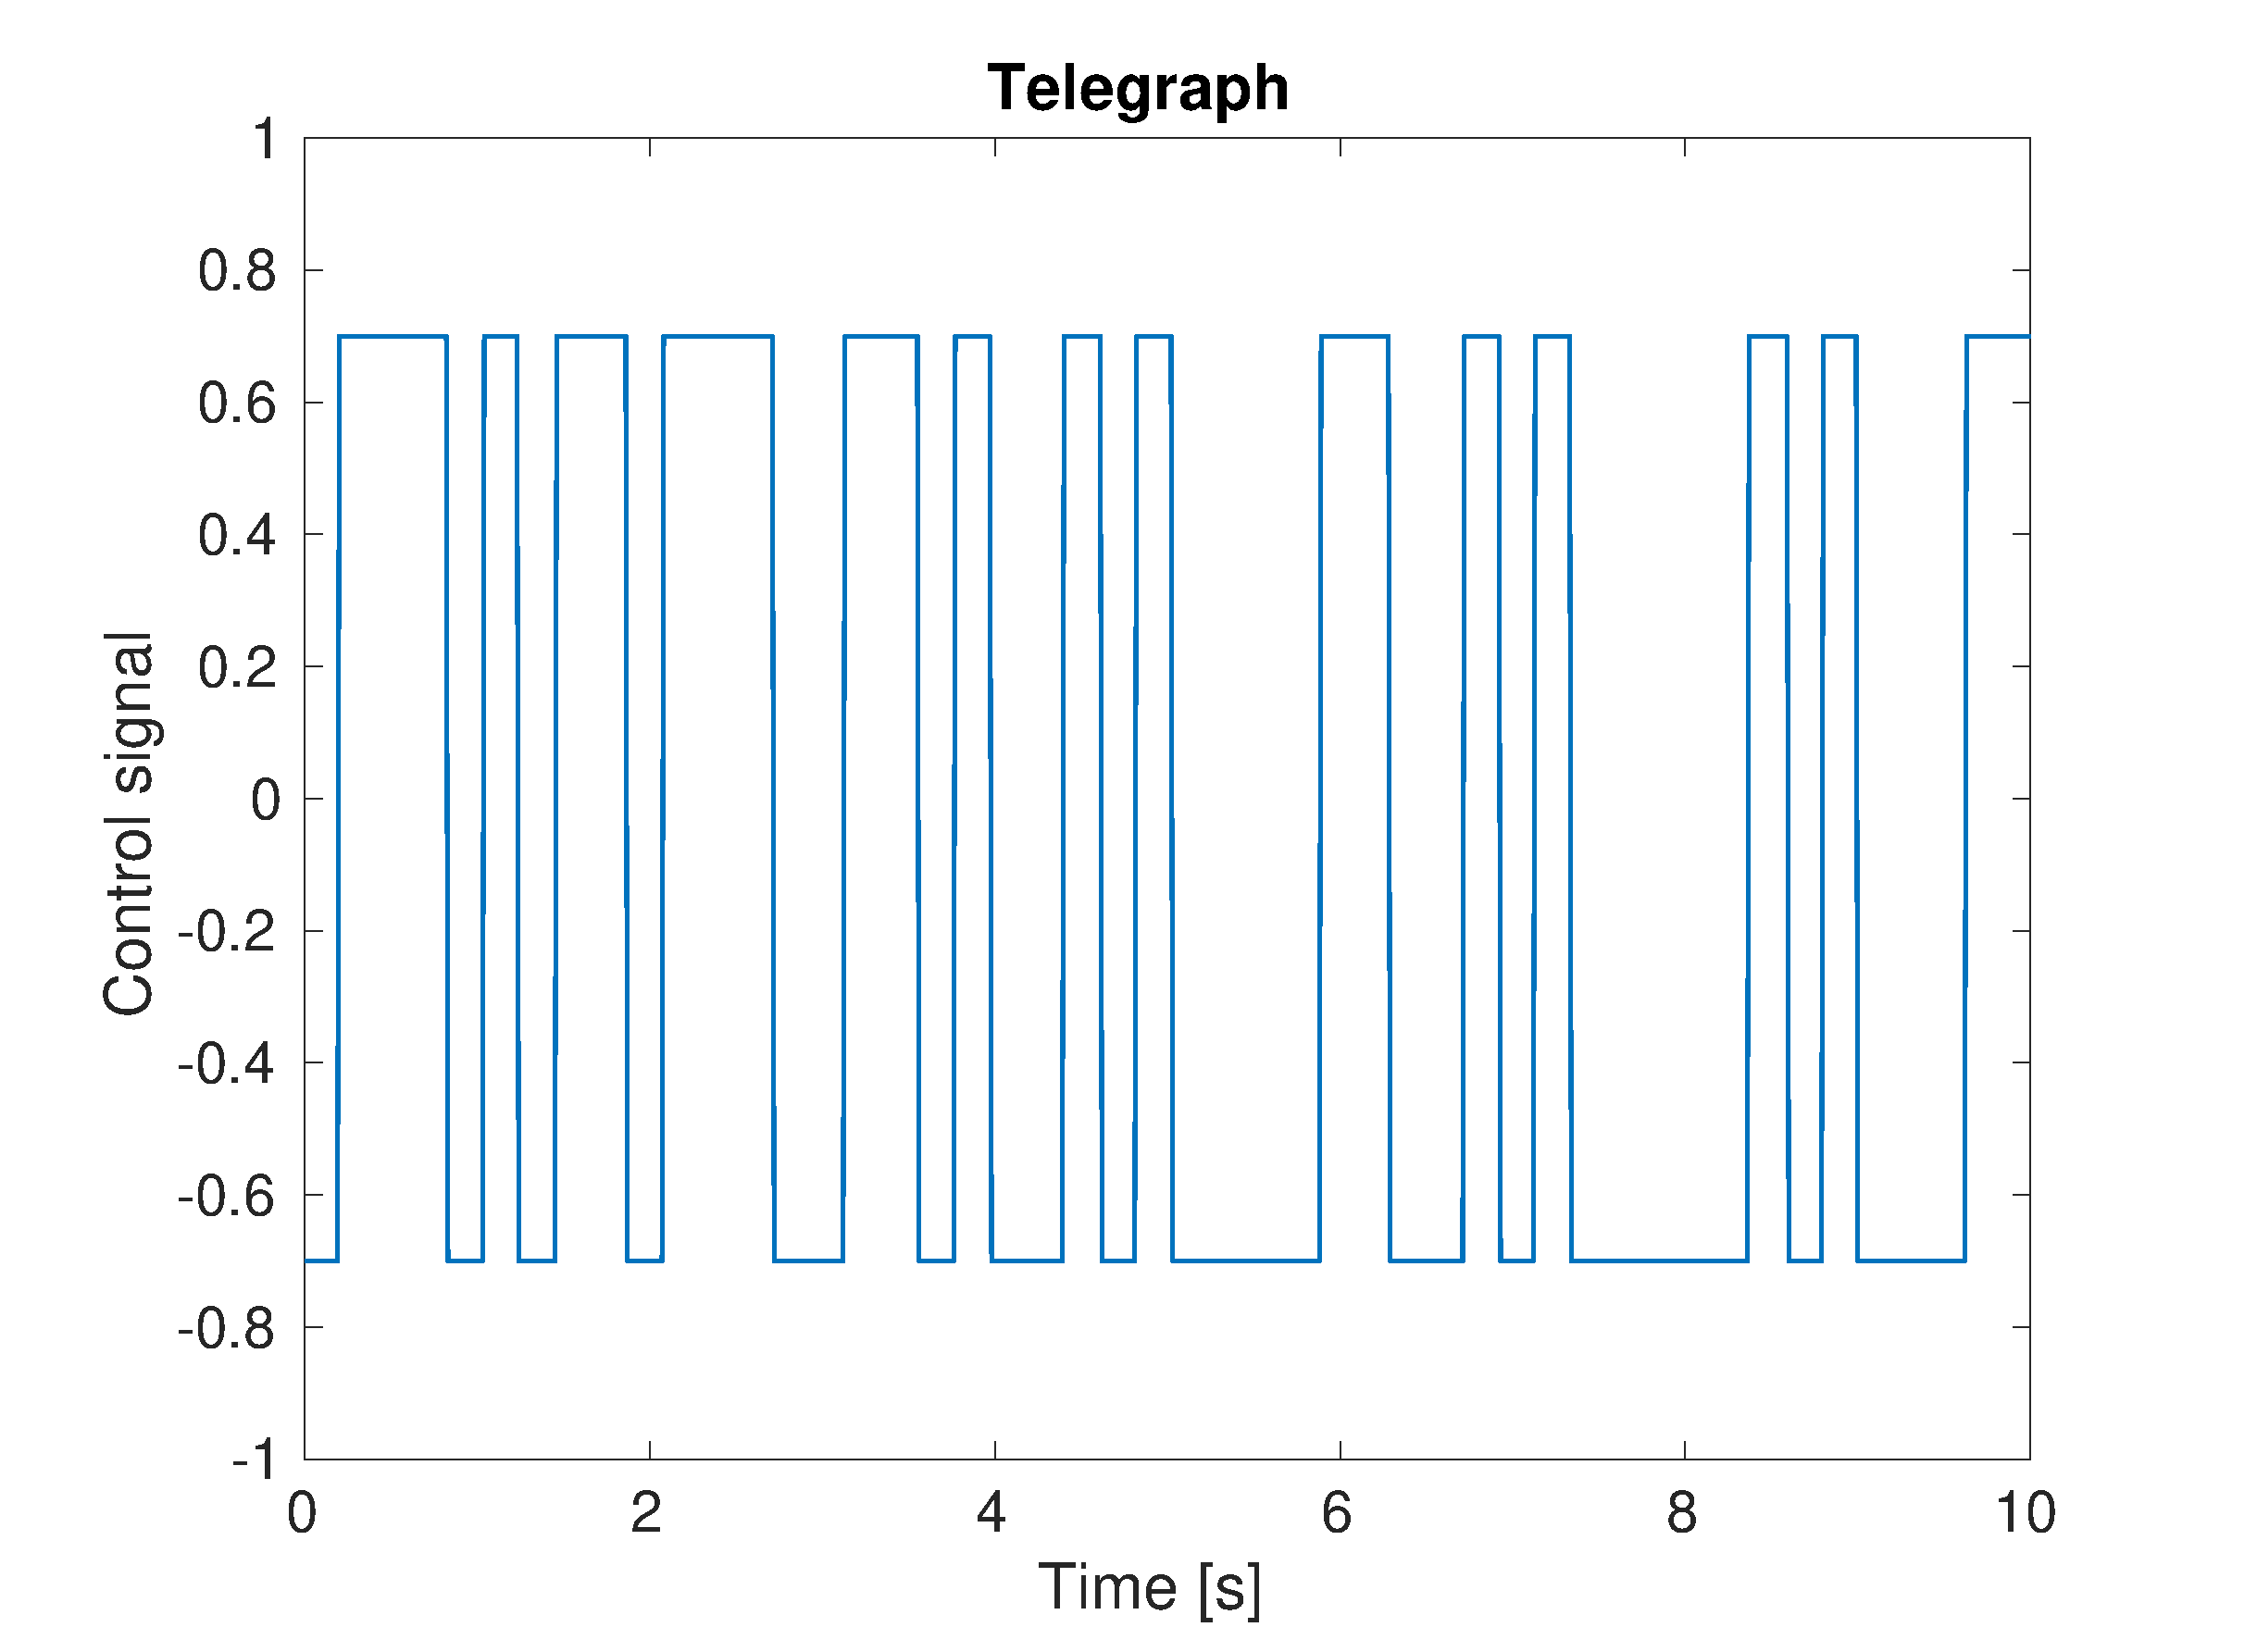
\includegraphics[width=0.8\textwidth]{telegraph}
\caption{An example of a telegraph signal which was sent to a thruster during data collection experiments.}
\label{fig:telegraph}
\end{figure}

Data preprocessing was done by synchronising the data streams by checking the start and end times of each experiment, here chosen as the time of arrival of the first control signal. The sensor data was aligned such that the data sample of each sensor whose arrival time was closest to the starting time of the test was chosen as the initial sample of each data stream. Data outside the test interval was discarded. After alignment the data was resampled to 100 Hz. The sensor data was resampled using first-order hold while the control signals were resampled using zero-order hold since the control signal data only contained points were the control signals changed.  

\begin{figure}[htbp]
  \centering
  \subfloat[][\label{fig:p_pqTest}Excitation in $p$ during $p$ and $q$ test.]{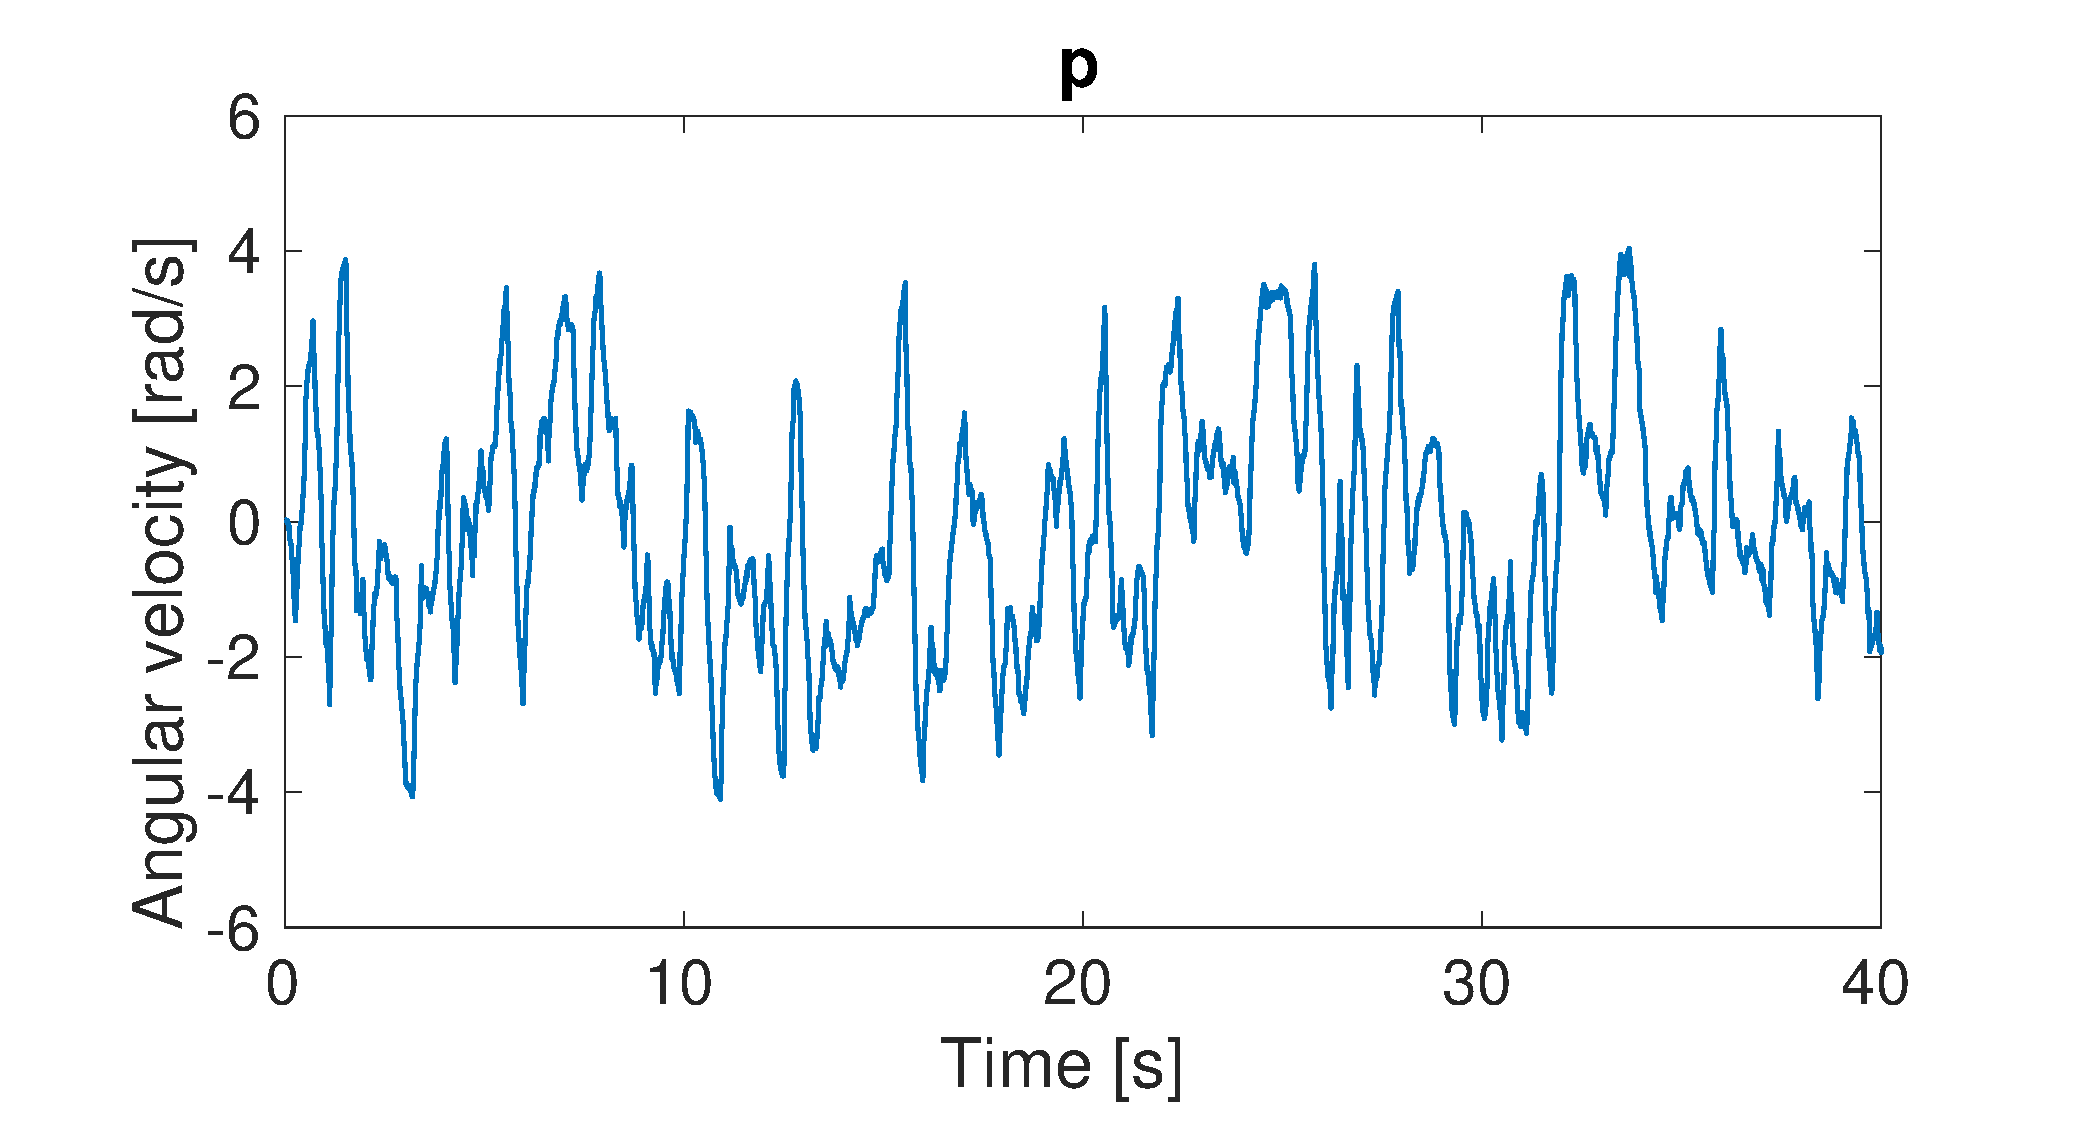
\includegraphics[width=0.4\textwidth]{p_pq_test}}
  \qquad
  \subfloat[][\label{fig:q_pqTest}Excitation in $q$ during $p$ and $q$ test.]{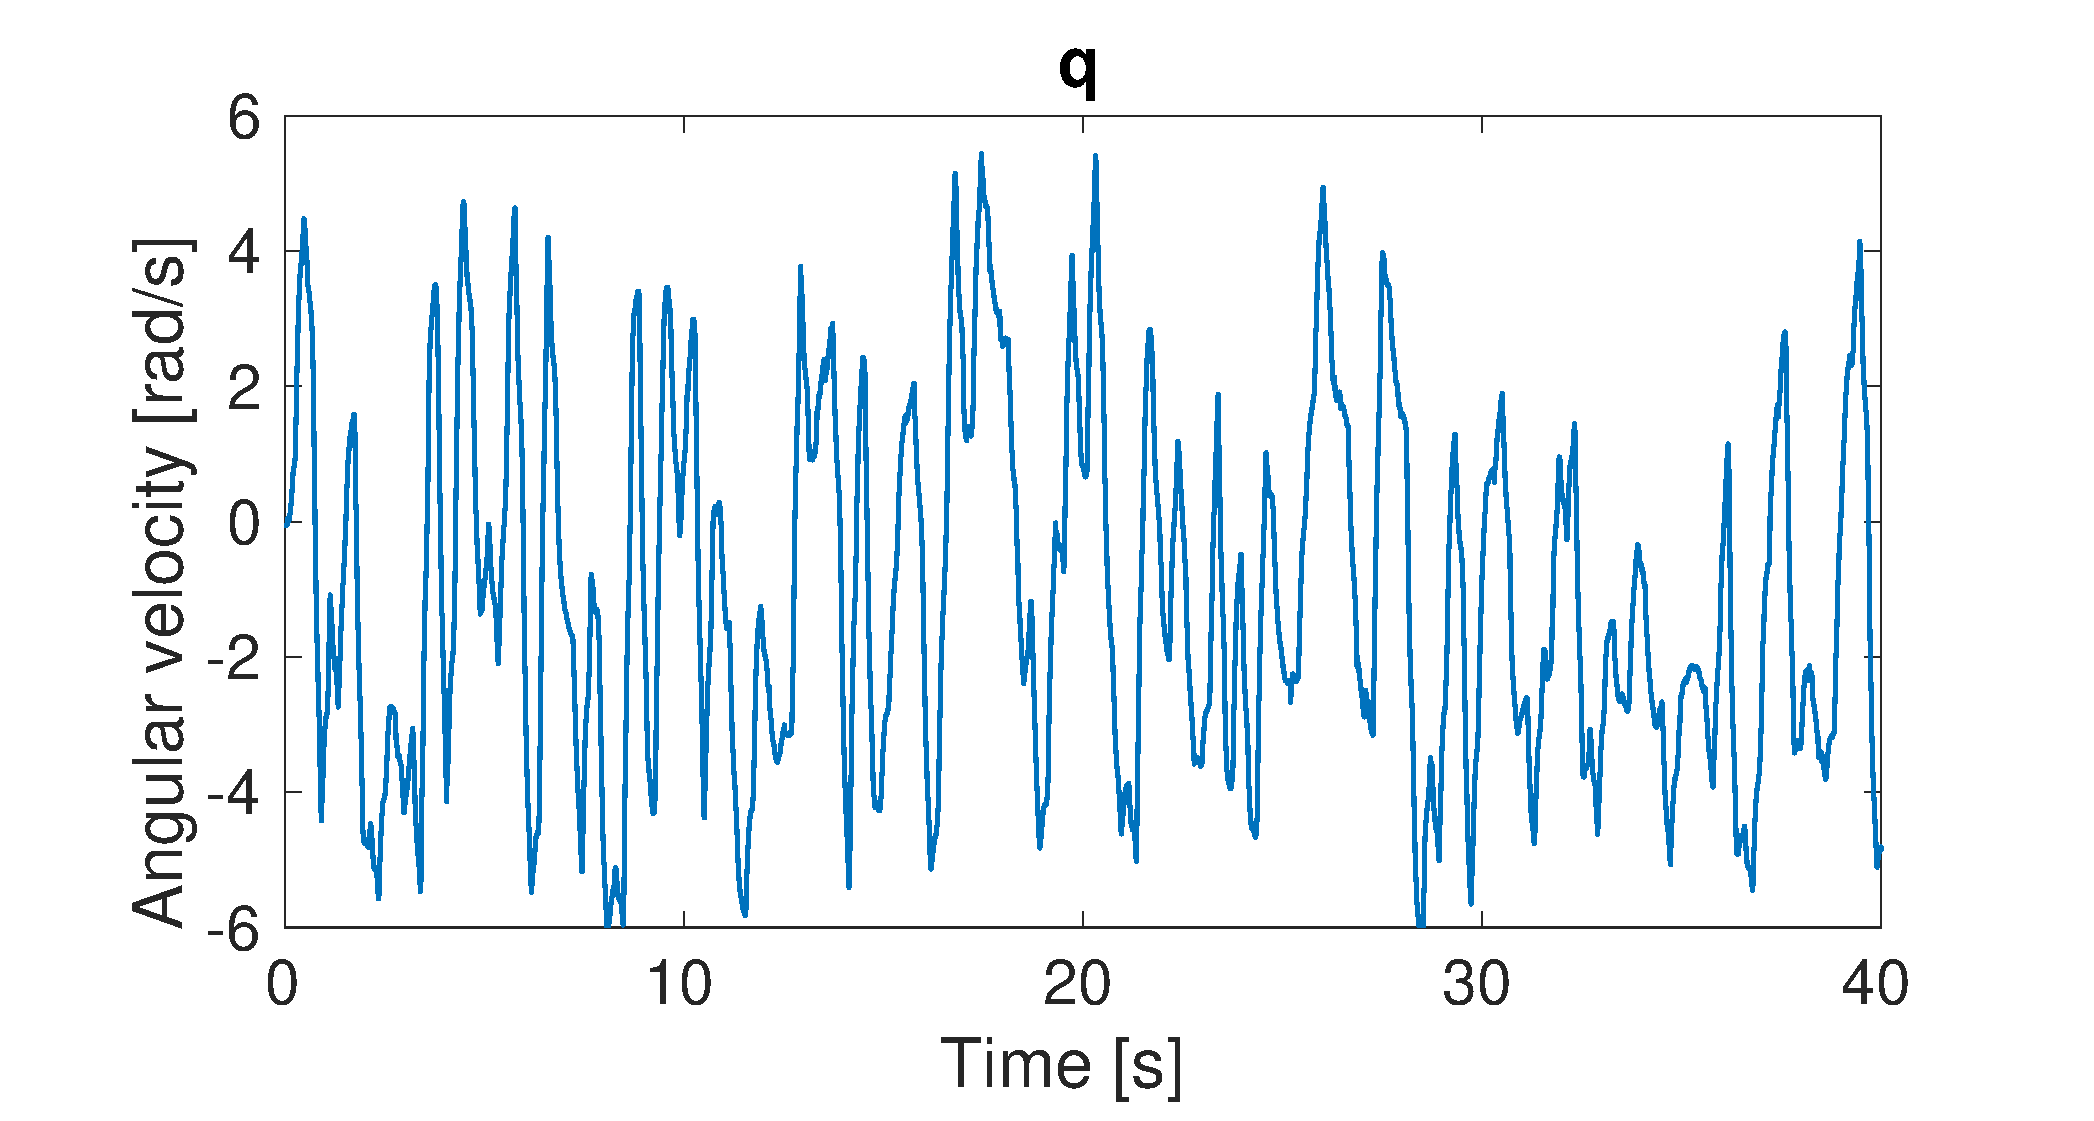
\includegraphics[width=0.4\textwidth]{q_pq_test}}
  \\
  \subfloat[][\label{fig:r_pqTest}Excitation in $r$ during $p$ and $q$ test.]{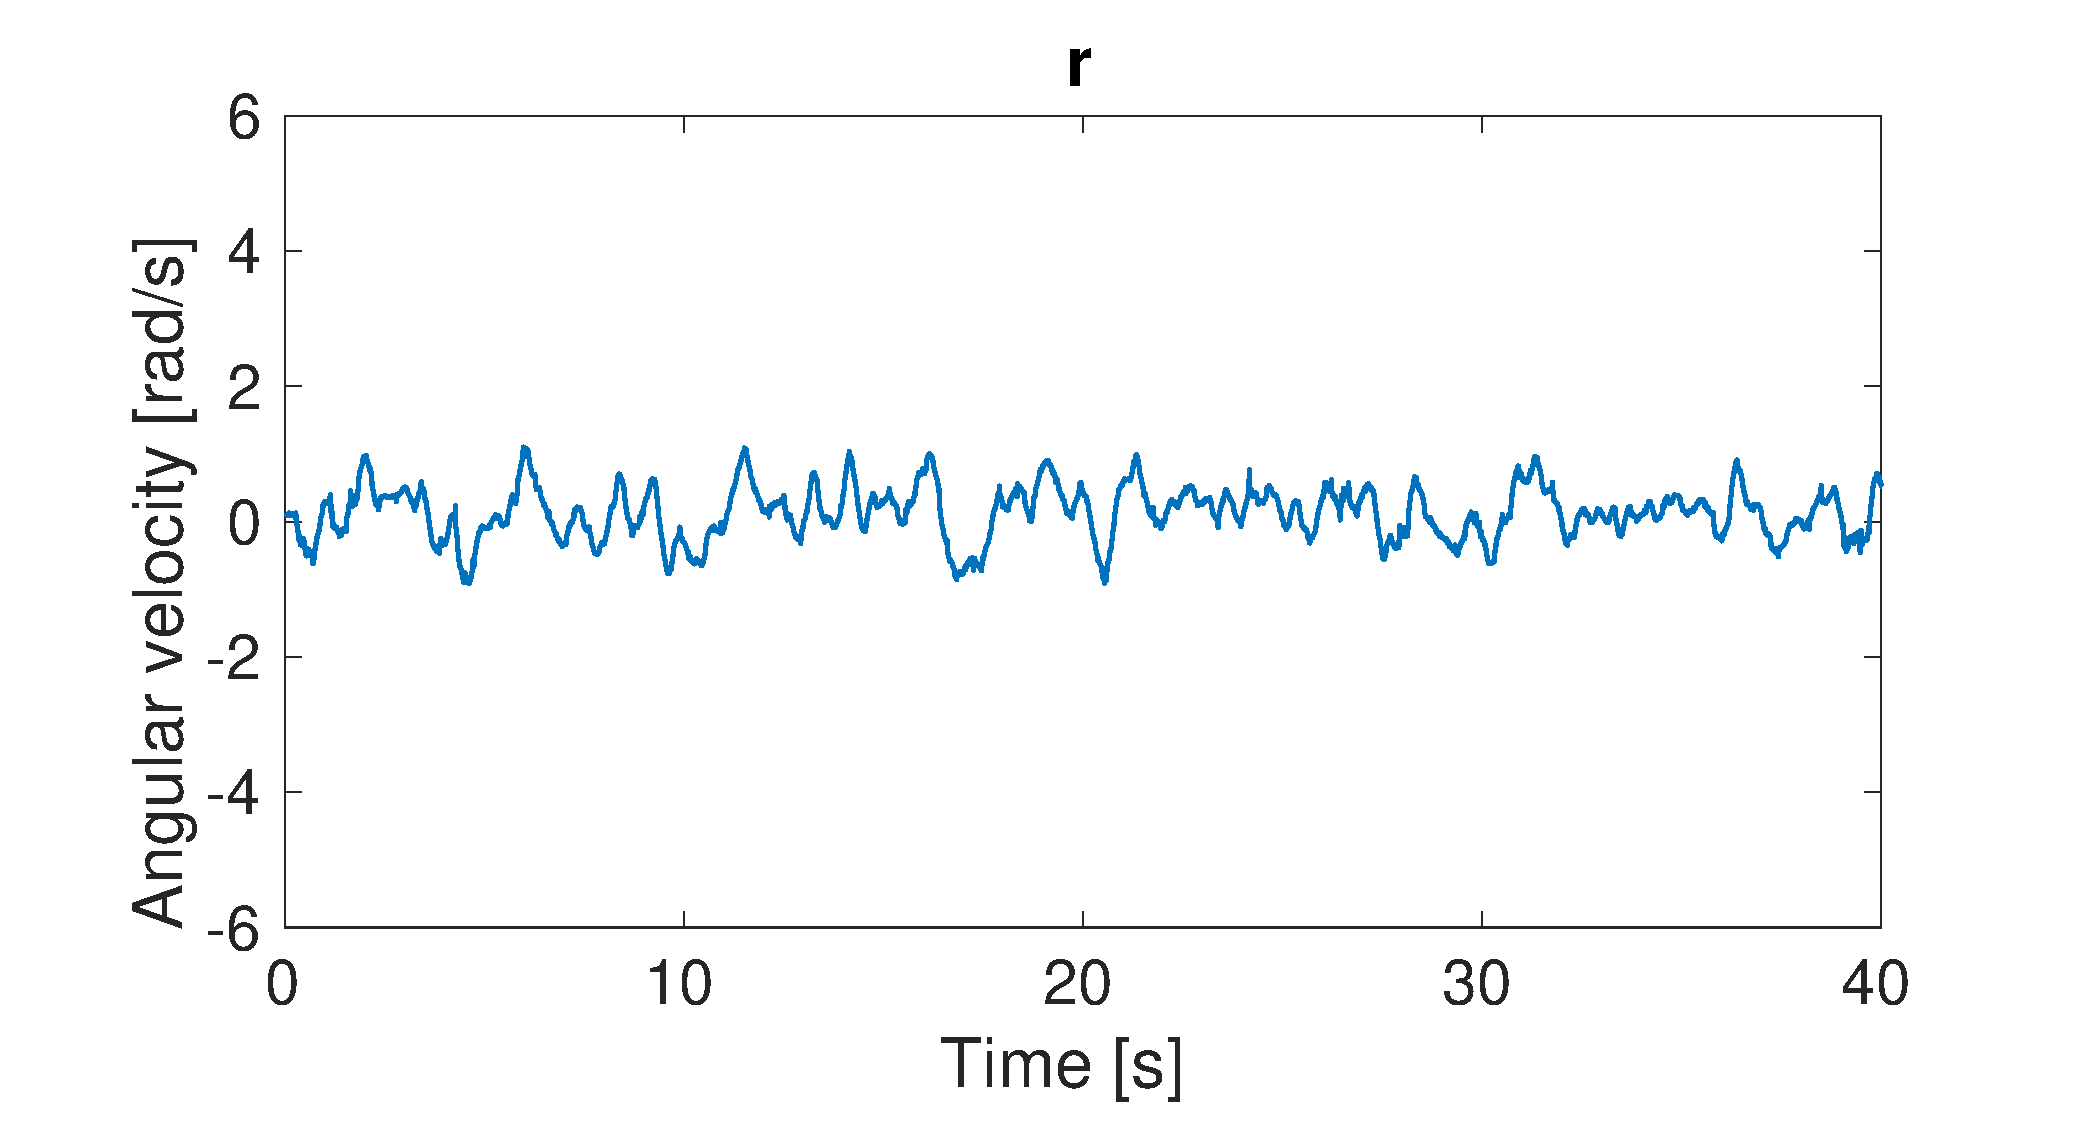
\includegraphics[width=0.4\textwidth]{r_pq_test}}
  \caption{\label{fig:pqTest}%
 Plots of excitation of the three angular velocities $p$, $q$ and $r$ from a test intended to mainly excite $p$ and $q$. Note that the amplitude in $r$ is four times smaller than that of $p$ and $q$.}
\end{figure}

\begin{figure}[htbp]
  \centering
  \subfloat[][\label{fig:p_rTest}Excitation in $p$ during $r$ test.]{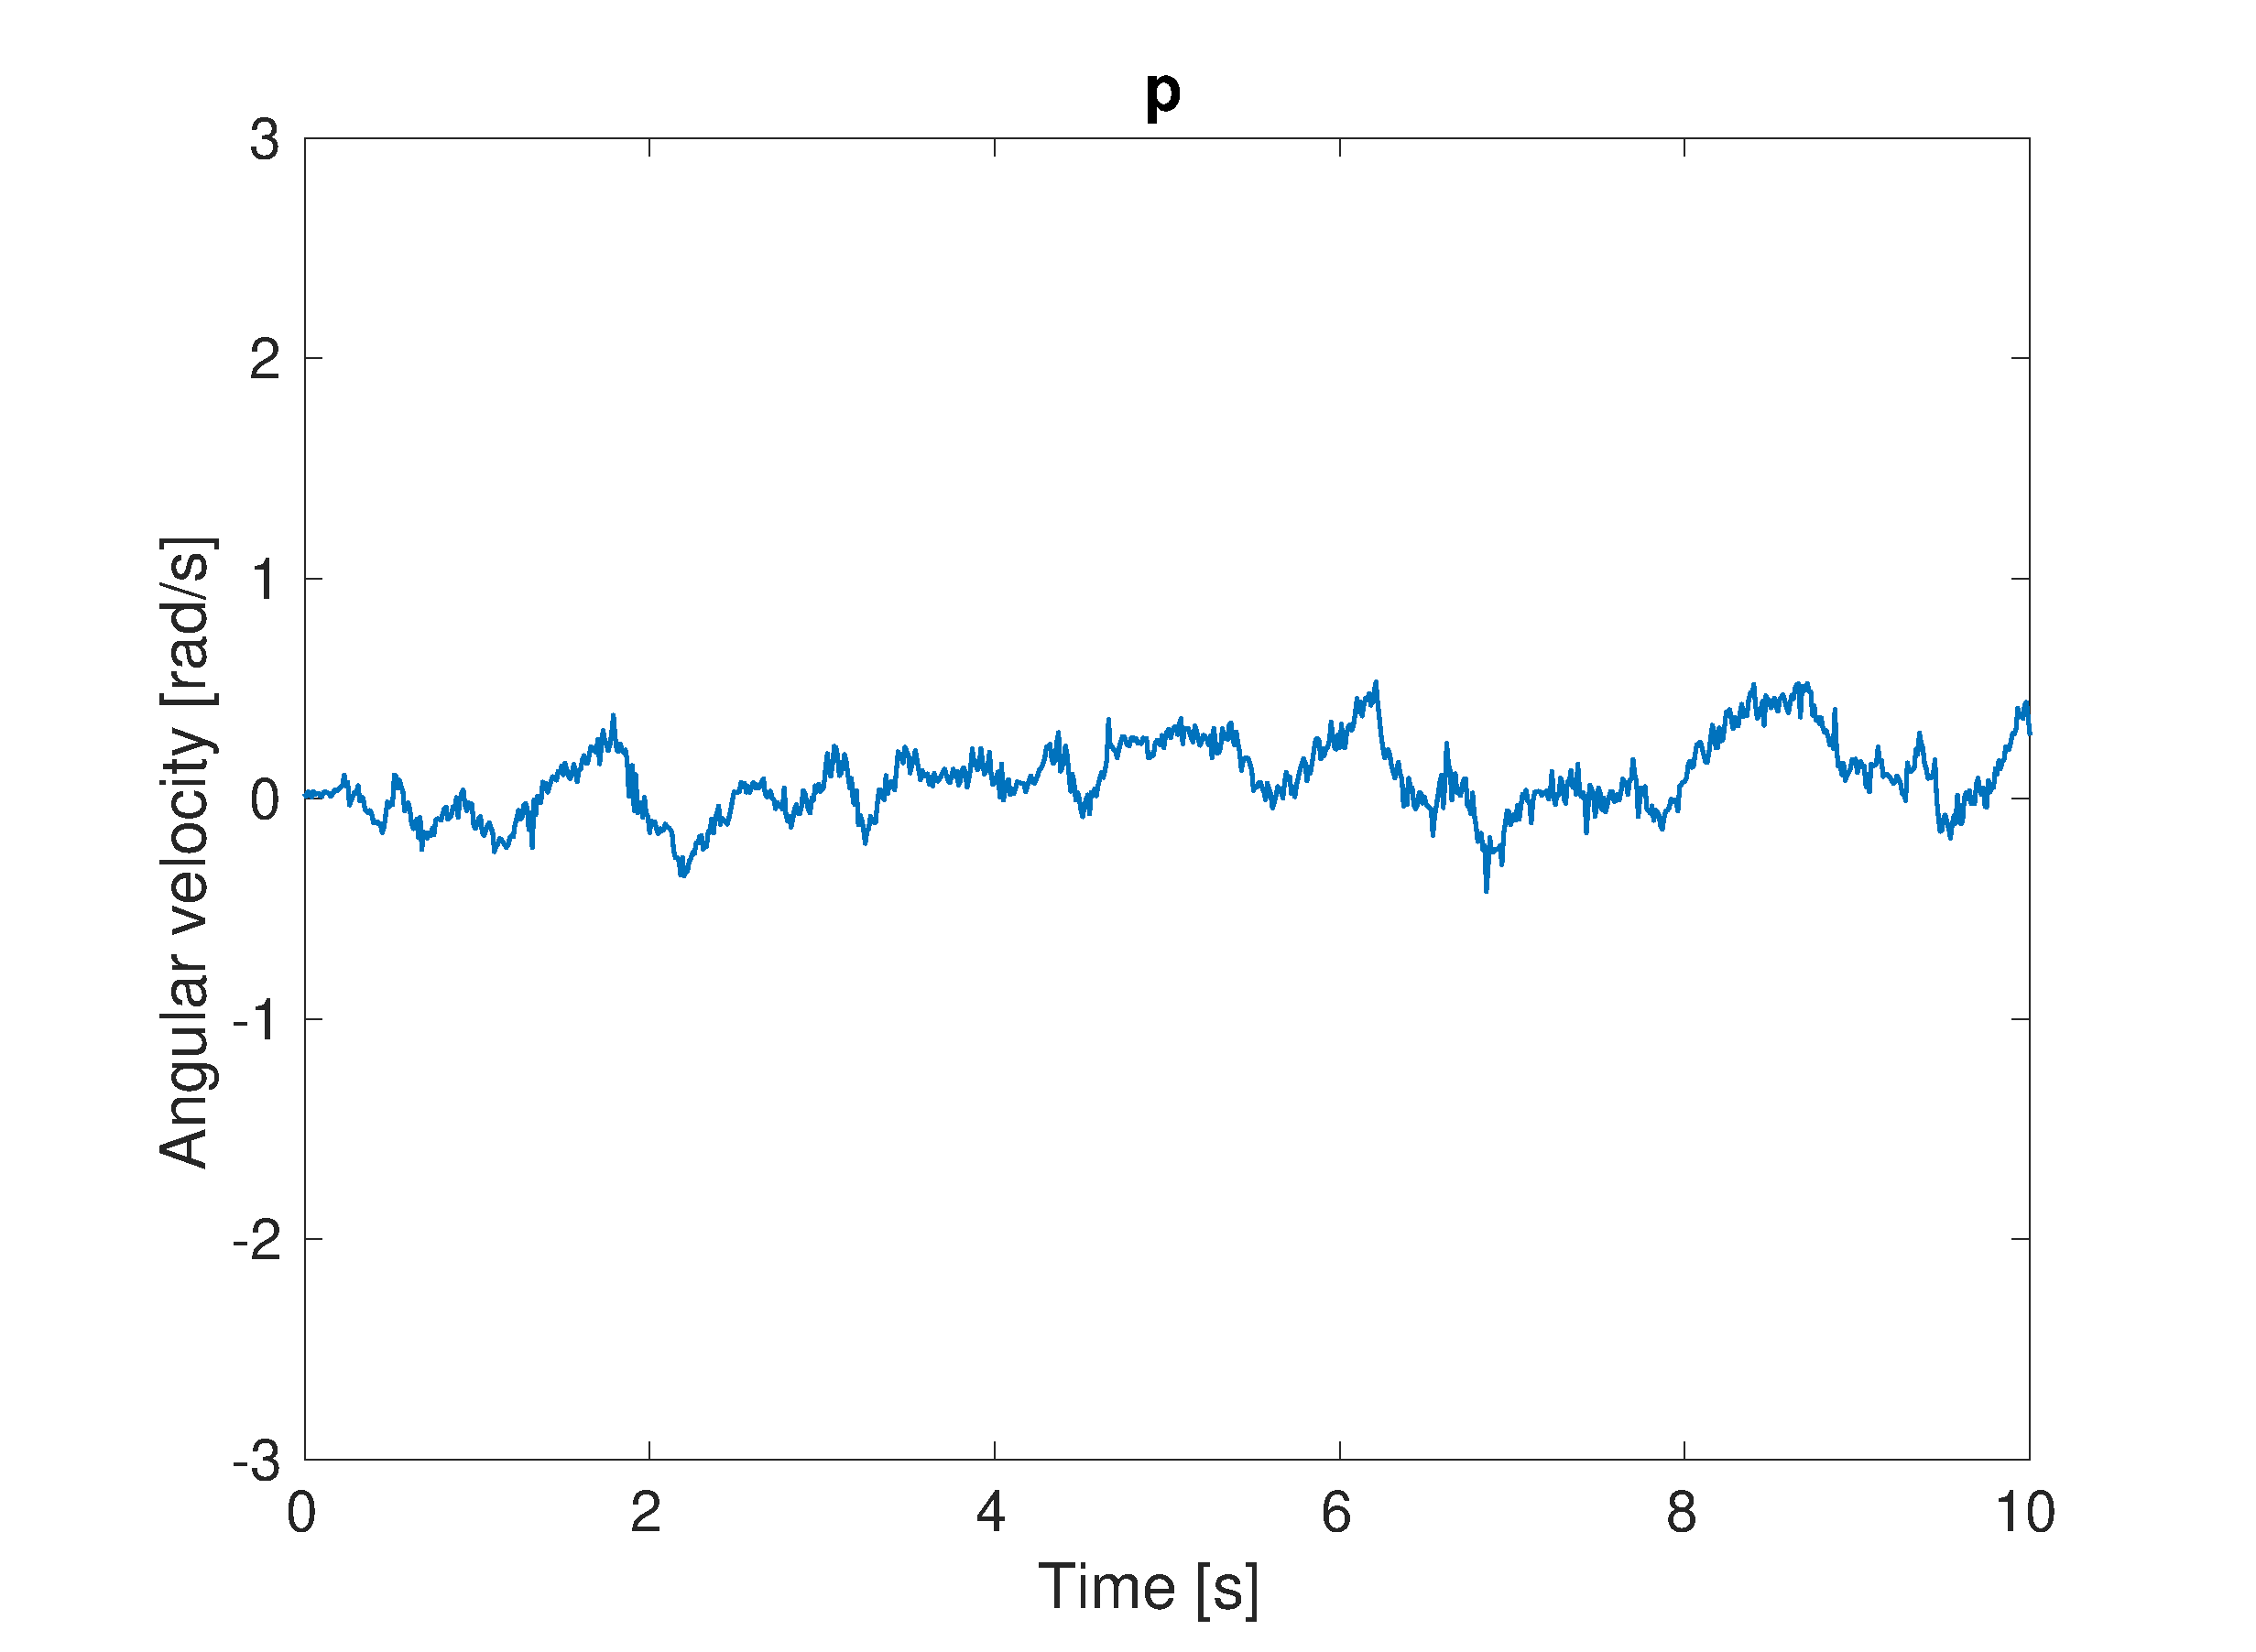
\includegraphics[width=0.4\textwidth]{p_r_test}}
  \qquad
  \subfloat[][\label{fig:q_rTest}Excitation in $q$ during $r$ test.]{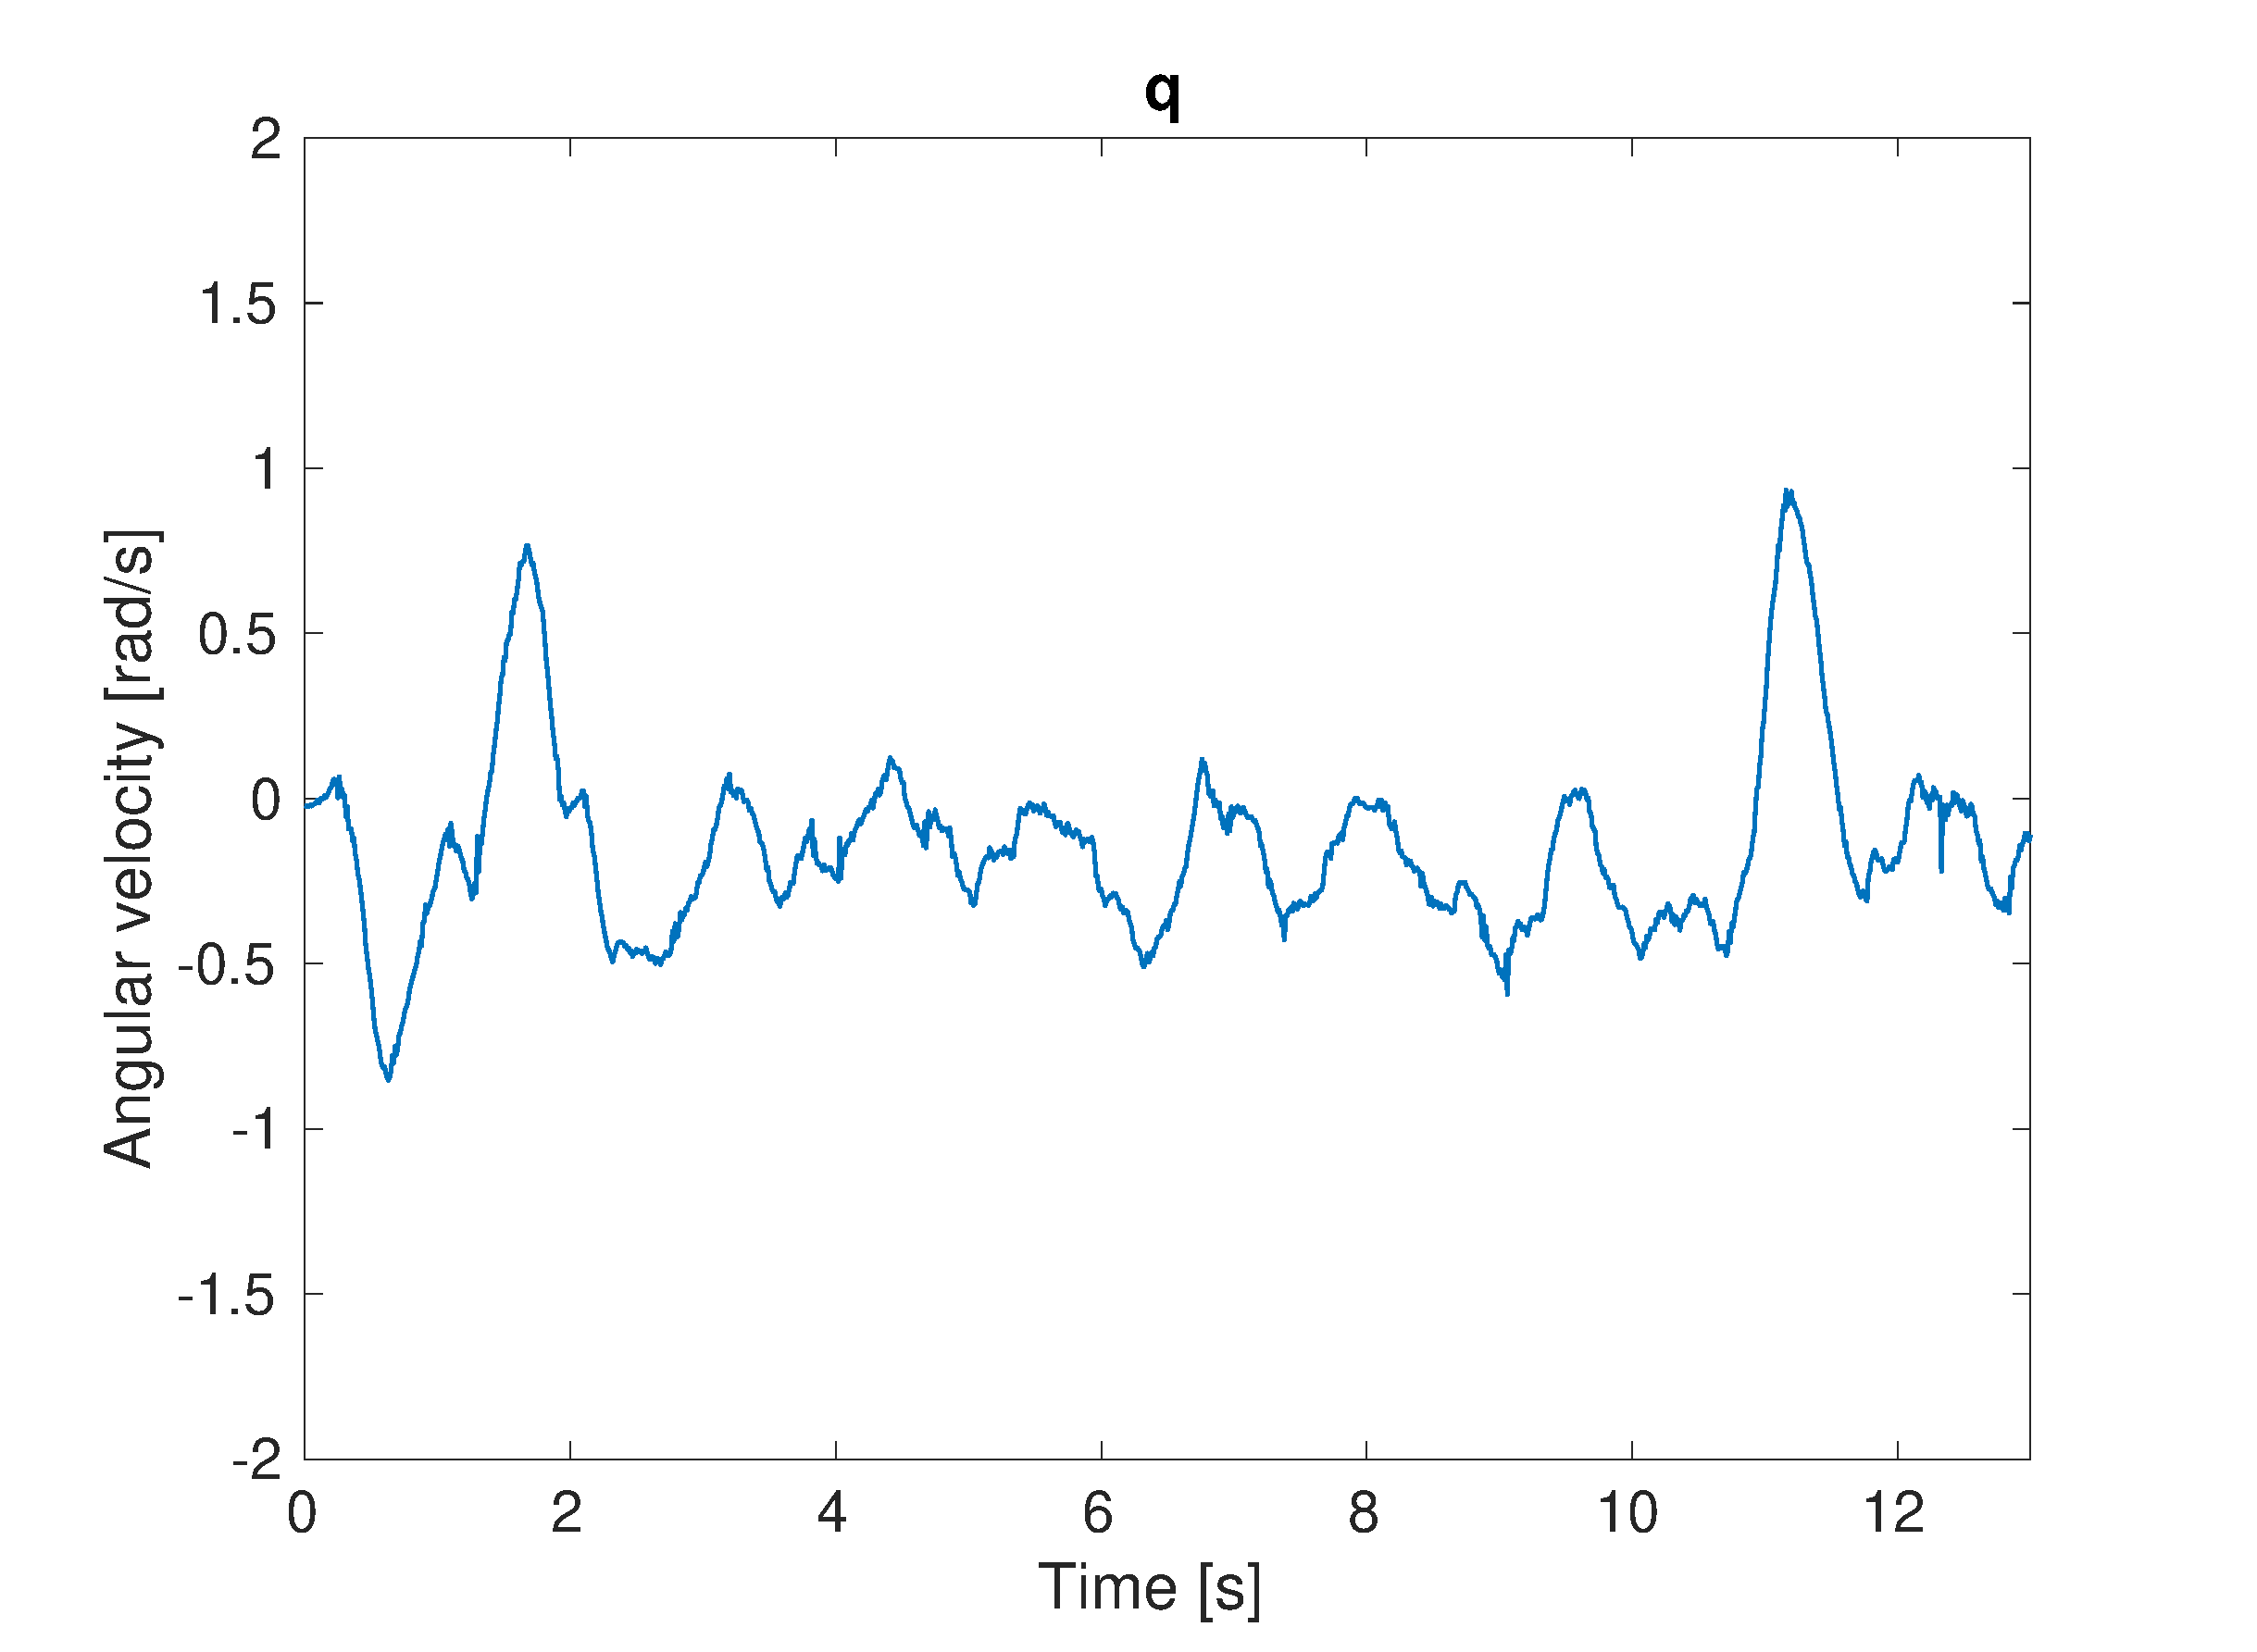
\includegraphics[width=0.4\textwidth]{q_r_test}}
  \\
  \subfloat[][\label{fig:r_rTest}Excitation in $r$ during $r$ test.]{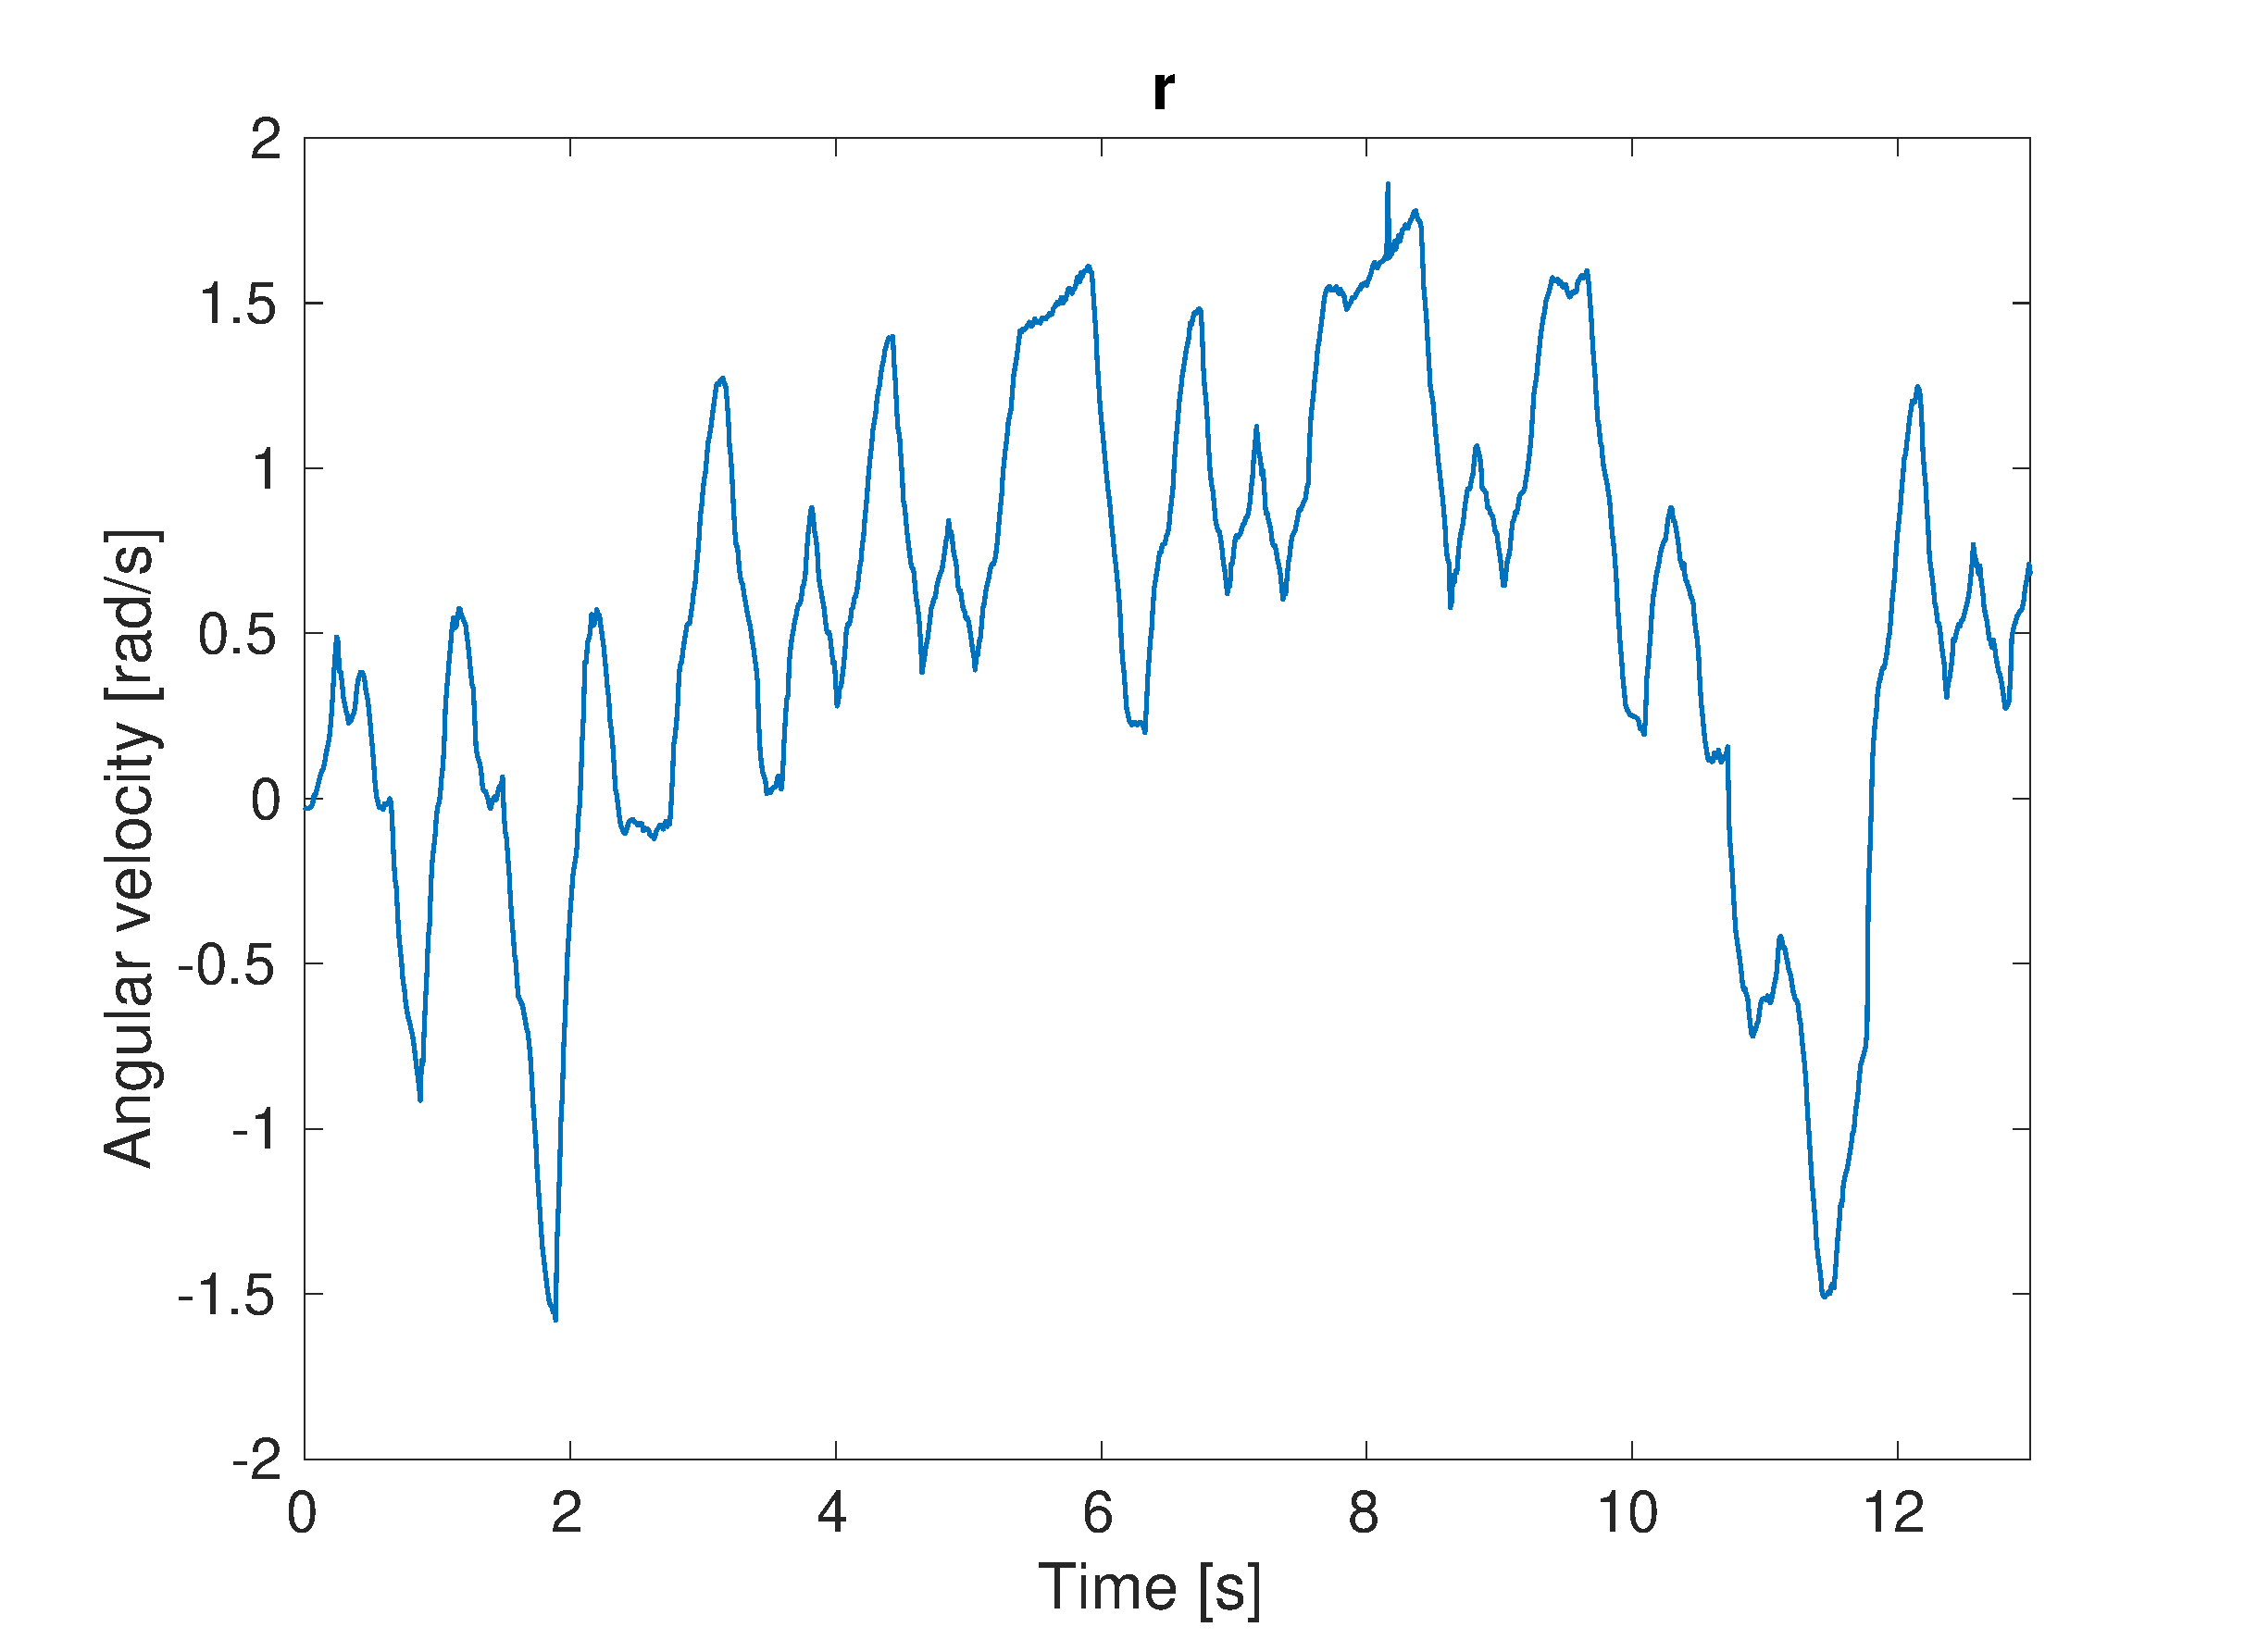
\includegraphics[width=0.4\textwidth]{r_r_test}}
  \caption{\label{fig:rTest}%
 Plots of excitation of the three angular velocities $p$, $q$ and $r$ from a test intended to mainly excite $r$. Note that the amplitude in $r$ is approximately two times larger than that of $p$ and $q$.}
\end{figure}
%%%%%%%%%%%%%%%%%%%%%%%%%%%%%%%%%

\section{Prediction-Error Method}
The prediction-error method uses a predictor $\hat{\boldsymbol{y}}_k(\boldsymbol{\theta})$ of a systems output to compare with the present output of the system. The discrete-time predictor can be described by 
\begin{equation}
\hat{\boldsymbol{x}}_{k+1}(\theta) = f(\boldsymbol{\hat{x}_k}(\theta), \boldsymbol{u}_k,\boldsymbol{y}_k, \boldsymbol{\theta})
\end{equation}
and
\begin{equation}
\hat{\boldsymbol{y}}_k(\boldsymbol{\theta}) = h(\hat{\boldsymbol{x}}_k, \boldsymbol{u}_k, \boldsymbol{\theta})
\end{equation}
where $\hat{\boldsymbol{x}}$ is the estimated state vector, $\boldsymbol{u}$ are the inputs and $\hat{\boldsymbol{y}}_k(\boldsymbol{\theta})$ is the predicted output of the model \citep[p. 13]{Roger}. 

The fitting is done by minimising a cost function $V(\boldsymbol{\theta})$ with respect to the parameter vector $\boldsymbol{\theta}$ \emph{i.e.}
\begin{equation}
\hat{\boldsymbol{\theta}} = \underset{\boldsymbol{\theta}}{\argmin} V(\boldsymbol{\theta})
\end{equation}
The cost function in this thesis has been defined as the squared error with an error threshold to handle noisy signals. An error threshold means that after a breakpoint the cost function becomes linear instead of quadratic, which makes the parameter estimation less sensitive to outliers. To reduce the impact of the noise even further, the used weight matrix in the quadratic cost function was chosen as the inverse of the estimated noise covariance. The cost function is then
\begin{equation}
    V(\boldsymbol{\theta}) = \frac{1}{N} \left( \sum_{t \in i} \boldsymbol{e}^T_k(\boldsymbol{\theta}) \boldsymbol{W}(\boldsymbol{\theta})  \boldsymbol{e}_k(\boldsymbol{\theta}) + \sum_{t \in j} \boldsymbol{v}^T_k(\boldsymbol{\theta}) \boldsymbol{W}(\boldsymbol{\theta})  \boldsymbol{v}_k(\boldsymbol{\theta}) \right)
\end{equation}
where $N$ is the number of samples in the dataset, $\boldsymbol{e}_k(\boldsymbol{\theta})$ is the error vector with the parameter vector~$\boldsymbol{\theta}$ and $\boldsymbol{W}$ is a positive definite weight matrix \citep{ljungtheory}. The set $i$ is the subset of errors for which $\abs{\boldsymbol{e}_k(\boldsymbol{\theta})} < \sigma \rho$ holds. Here, $\sigma$ is the estimated standard deviation of $\boldsymbol{e}_k(\boldsymbol{\theta})$ and $\rho$ is the chosen error threshold. The set $j$ is the complement of $i$. The error $\boldsymbol{v}_k(\boldsymbol{\theta})$ is defined as 
\begin{equation}
\boldsymbol{v}_k(\boldsymbol{\theta}) = \boldsymbol{e}_k(\boldsymbol{\theta}) \sigma\frac{\rho}{\sqrt{\abs{\boldsymbol{e}_k(\boldsymbol{\theta})}}}
\end{equation}

%Several tools exists	which can estimate parameters using the prediction-error method. In this thesis the System Identification Toolbox\texttrademark has been used.
%%%%%%%%%%%%%%%%%%%%%%%%%%%%%%%%%%%%%%%%%%%%%%%%%%%%%%%%%%%
\section{Estimation Using Prediction-Error Method}
A initial set of model parameters were estimated using \eqref{eq:pq_dot_decouple} and \eqref{eq:r_dot_decouple}, while using appropriate data sets. These initial parameters were then used in model \eqref{eq:quatModel}. Estimated angles were used as inputs and angular velocities as outputs. This gave the following model structure to be estimated
\begin{equation}
\dot{\hat{\boldsymbol{\eta}}} = f(\nuVector, \hat{\etaVector}, \tauVector)
\end{equation}
and
\begin{equation}
\hat{\boldsymbol{y}} = \nuVector + \boldsymbol{v}_{\text{Meas}}
\end{equation}
where $\hat{\etaVector}$ are the estimated Euler angles from the sensor fusion and $\boldsymbol{v}_{\text{Meas}}$ are measurement noise.
The result of the estimation can be seen in \Tableref{tab:ResultEstimAngular}.  The fit of the model compared to validation data can be seen in \Figureref{fig:velocityCompareCong}. The model has a high fit of $50-60\ \%$ and thus describes the validation data well.
%The estimation used two datasets as estimation data and used one dataset for validation data.%
\begin{figure}[tbp]
  \centering
  \subfloat[][\label{fig:velocityCompareCongp}Simulated model and validation data in $p$.]{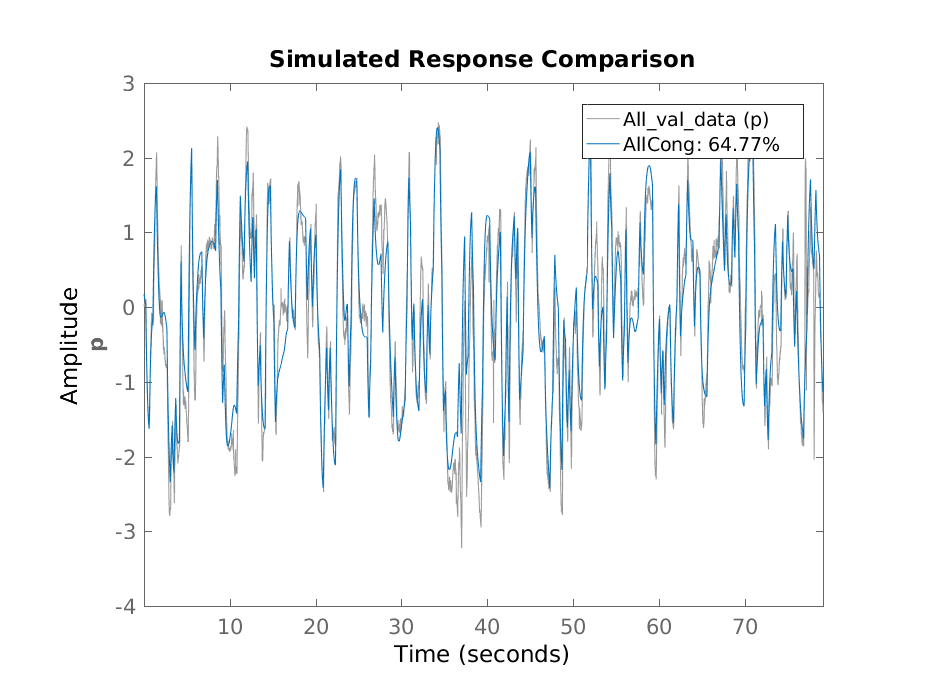
\includegraphics[width=0.4\textwidth]{velocityCompareCongp}}
  \qquad
  \subfloat[][\label{fig:velocityCompareCongq}Simulated model and validation data in $q$.]{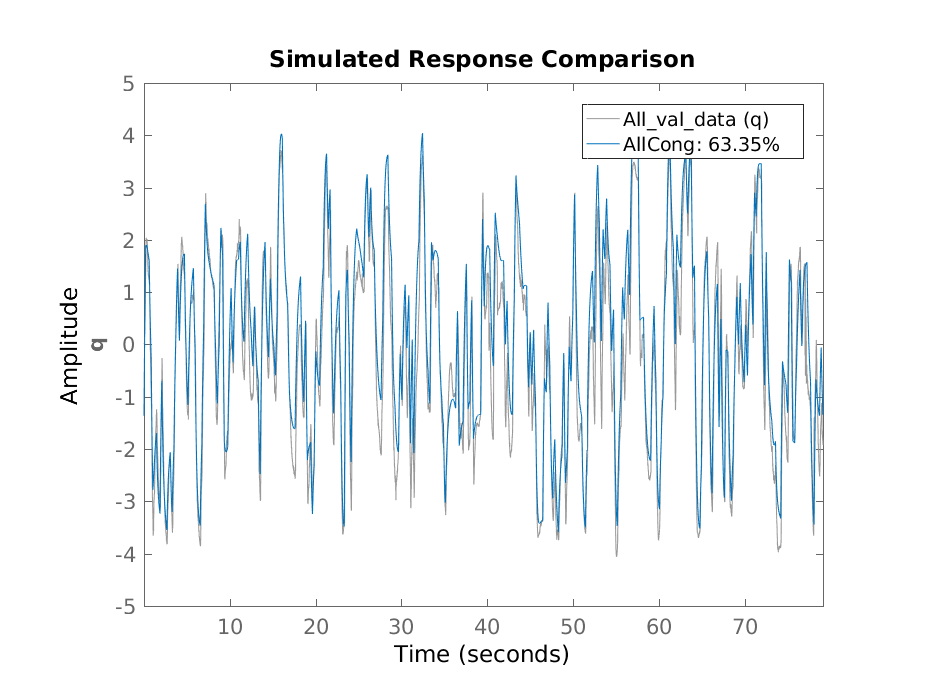
\includegraphics[width=0.4\textwidth]{velocityCompareCongq}}
  \\
  \subfloat[][\label{fig:velocityCompareCongr}Simulated model and validation data in $r$.]{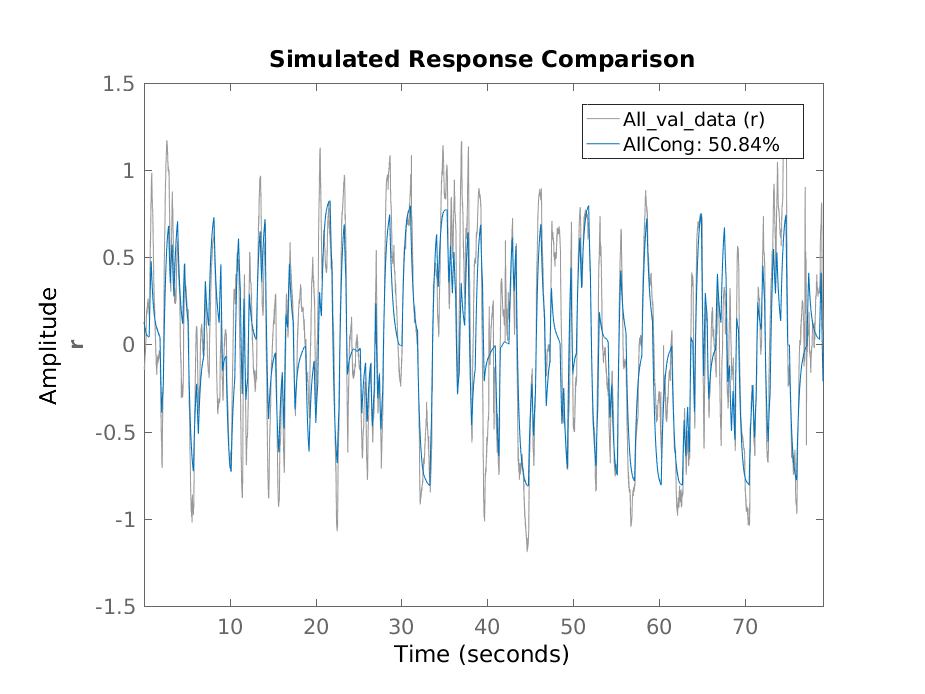
\includegraphics[width=0.4\textwidth]{velocityCompareCongr}}
  \caption{\label{fig:velocityCompareCong}%
    Comparison of simulation of the attitude model (blue) against validation data (gray) using the estimated angels as inputs and angular velocities as outputs. The simulated model has a high fit compared to the validation data.}
\end{figure}

The estimate of $\etaVector$ did not follow the kinematic relations described in \sectionref{sec:coordinates}. The problem with $\etaVector$ not following the kinematic relations was further investigated by comparing integration of \eqref{eq:eulerAnglesdot} with $\hat{\etaVector}$ from the sensor fusion. As can be seen in \Figureref{fig:integratedAngleVelocities} the result was not satisfactory, with the estimated angles and the integration of \eqref{eq:eulerAnglesdot} being very dissimilar. It was therefore concluded that the estimated angles were unfit for use as outputs during parameter estimation unless a new motion model for the sensor fusion was created to solve the issue. It is therefore recommended that the validity of the observer is controlled using relations such as those in \sectionref{sec:coordinates} before collecting data. 

\begin{figure}[htbp]
  \centering
  \subfloat[][\label{fig:velocityAnglePhi}Comparison between integration of $\dot{\phi}$ and $\hat{\phi}$ from the \abbrEKF]{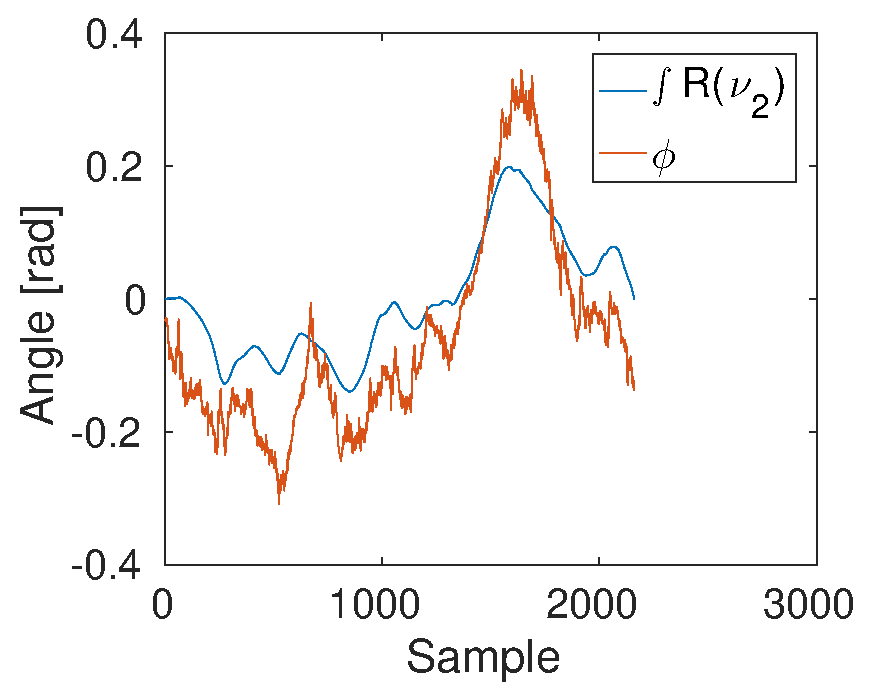
\includegraphics[width=0.4\textwidth]{velocityAnglePhi}}
  \qquad
  \subfloat[][\label{fig:velocityAngleTheta}Comparison between integration of $\dot{\theta}$ and $\hat{\theta}$ from the \abbrEKF]{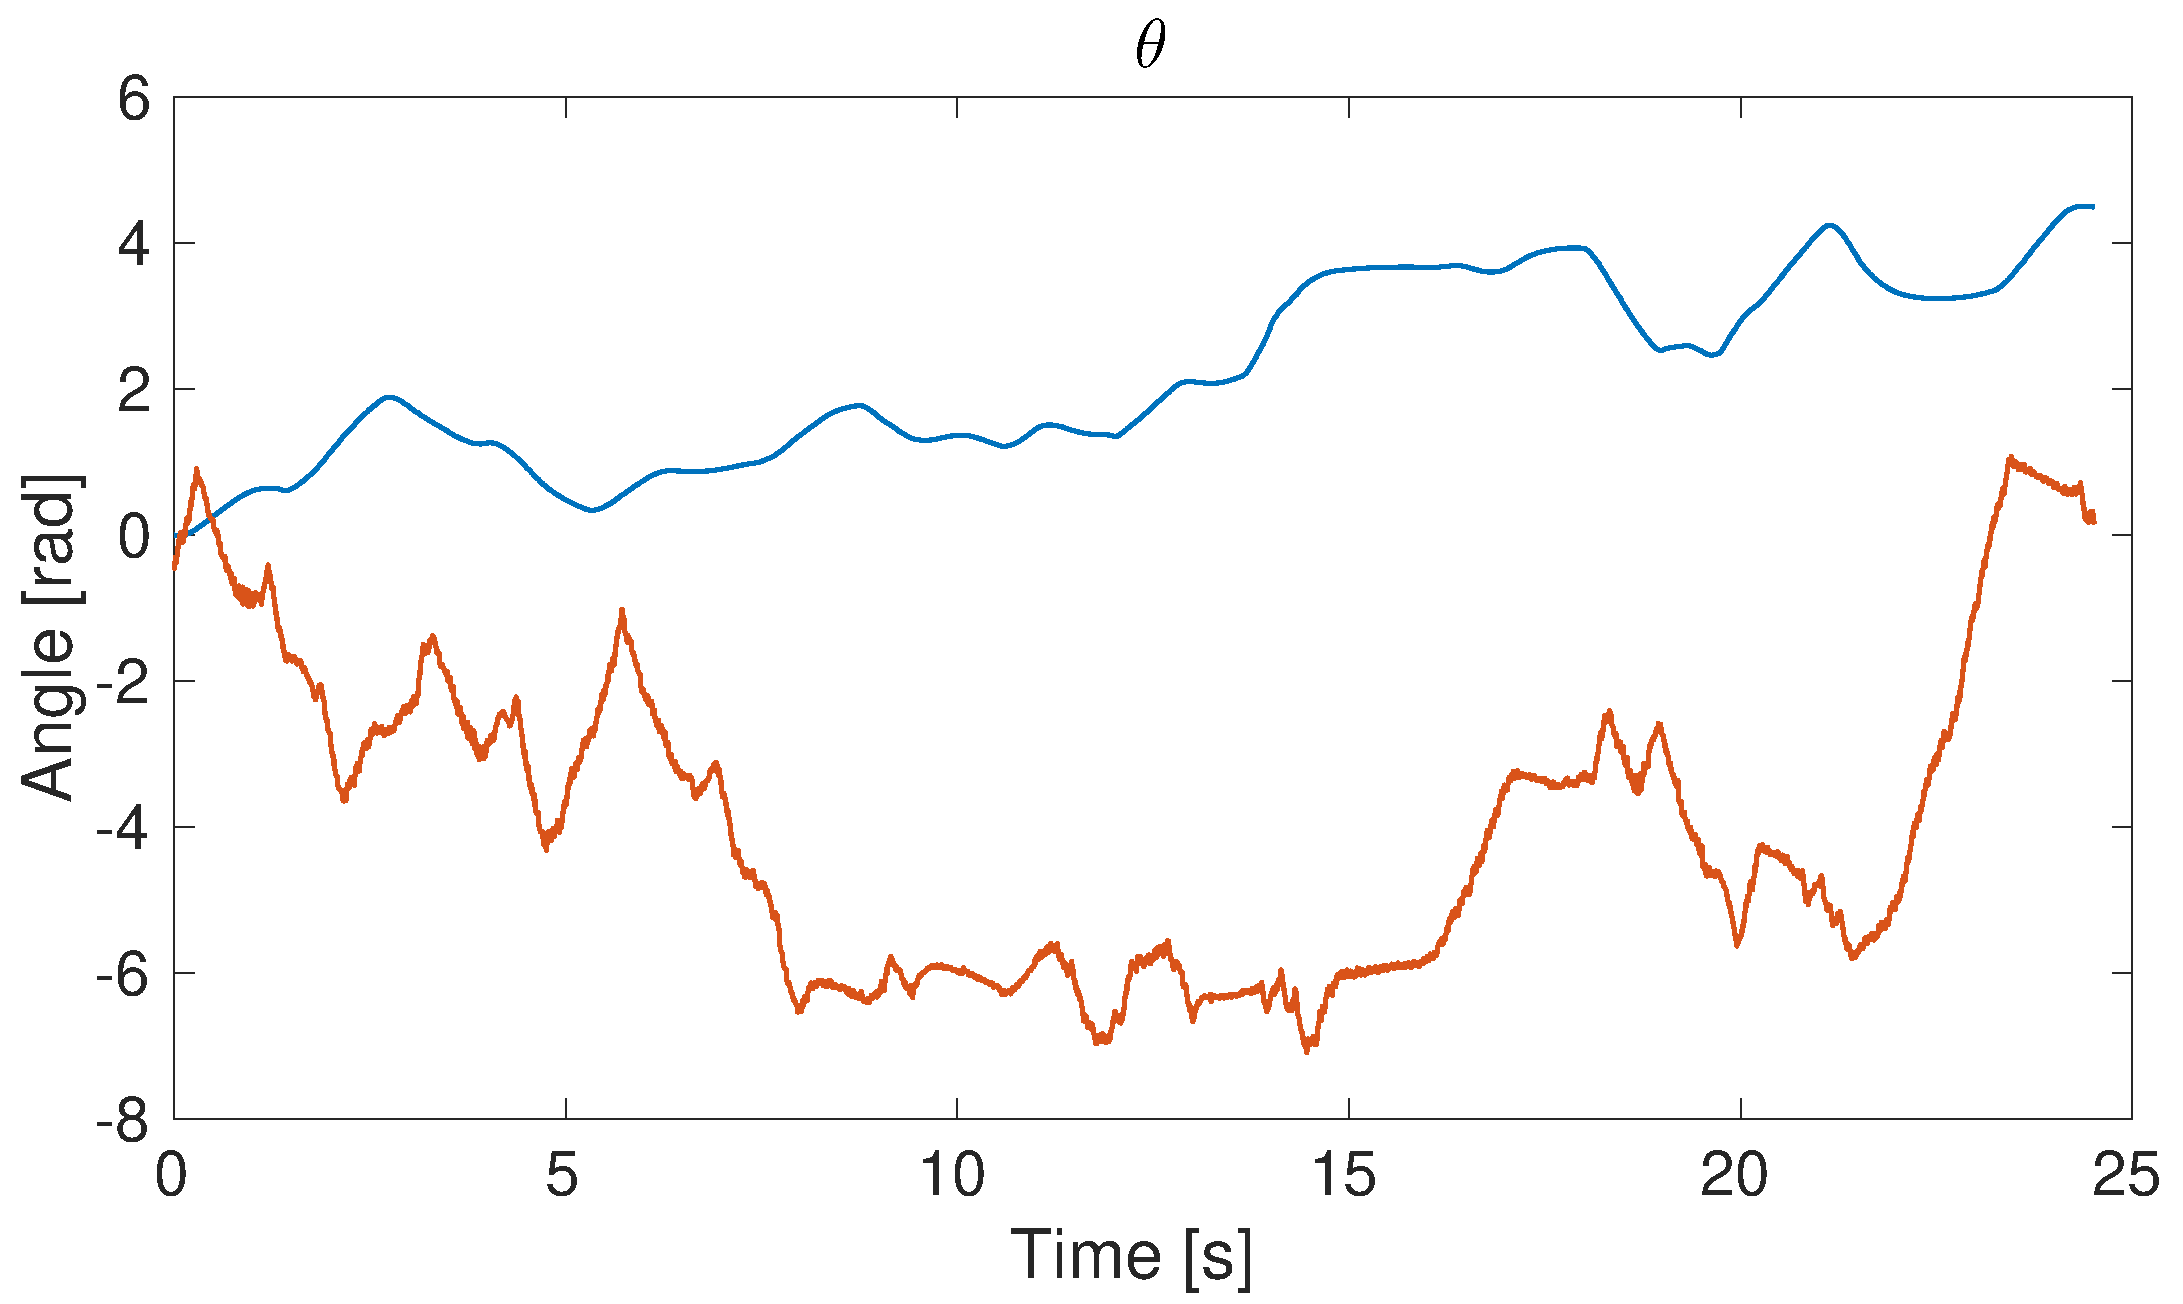
\includegraphics[width=0.4\textwidth]{velocityAngleTheta}}
  \\
  \subfloat[][\label{fig:velocityAnglePsi}Comparison between integration of $\dot{\psi}$ and $\hat{\psi}$ from the \abbrEKF]{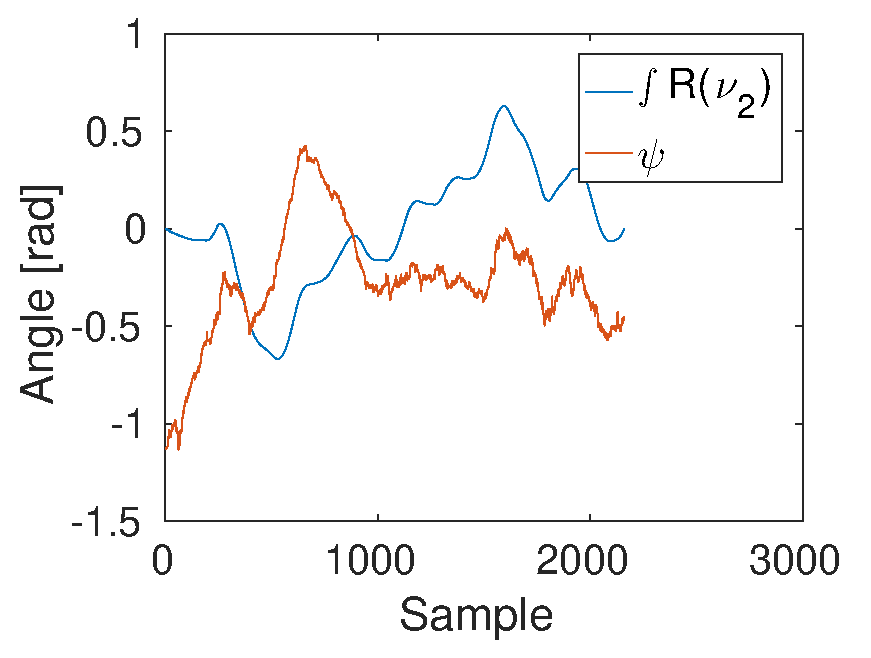
\includegraphics[width=0.4\textwidth]{velocityAnglePsi}}
  \caption{\label{fig:integratedAngleVelocities}%
  A comparison between integration of euler angles (blue) using \eqref{eq:eulerAnglesdot} and the estimated euler angles from the \abbrEKF (red). The angles are poorly estimated and thus not suitable to use as outputs in parameter estimation.}
\end{figure}

Due to the aforementioned problems, the model \eqref{eq:quatModel} was used with angular velocities and linear acceleration as outputs. Thus the estimation structure became
\begin{equation}
\dot{\hat{\etaVector}} = J(\hat{\etaVector}) \hat{\nuVector},
\end{equation}
\begin{equation}
\dot{\hat{\nuVector}} =  f(\hat{\etaVector}, \hat{\nuVector}, \tauVector)
\end{equation}
with 
\begin{equation}
\hat{\boldsymbol{y}} = \begin{pmatrix}
\hat{\nuVector} \\
\hat{\boldsymbol{a}}
\end{pmatrix}
\end{equation}
where $\hat{\boldsymbol{a}}$ is the estimated linear acceleration in the \abbrROV frame.
An issue that was encountered when estimating the parameters was that when angular velocities and linear accelerations were used as outputs, the model was extremely sensitive to the initial value of the quaternions. To examine this problem further, data was generated using a simulator and the simulated data was used in the estimation. The estimator was initialised with the correct initial parameter values from the simulator, but it was free to estimate the initial value of the quaternions. As expected, the estimated starting quaternion was not well estimated, which in turn led to the parameters diverging from their true values and a low fit was obtained. A result from such a test can be seen in \Figureref{fig:angVelSim}.

\begin{figure}[htbp]
  \centering %comparison betwwen two simulations
  \subfloat[][\label{fig:angVelSimp}Angular velocity around the \abbrROV's x-axis.]{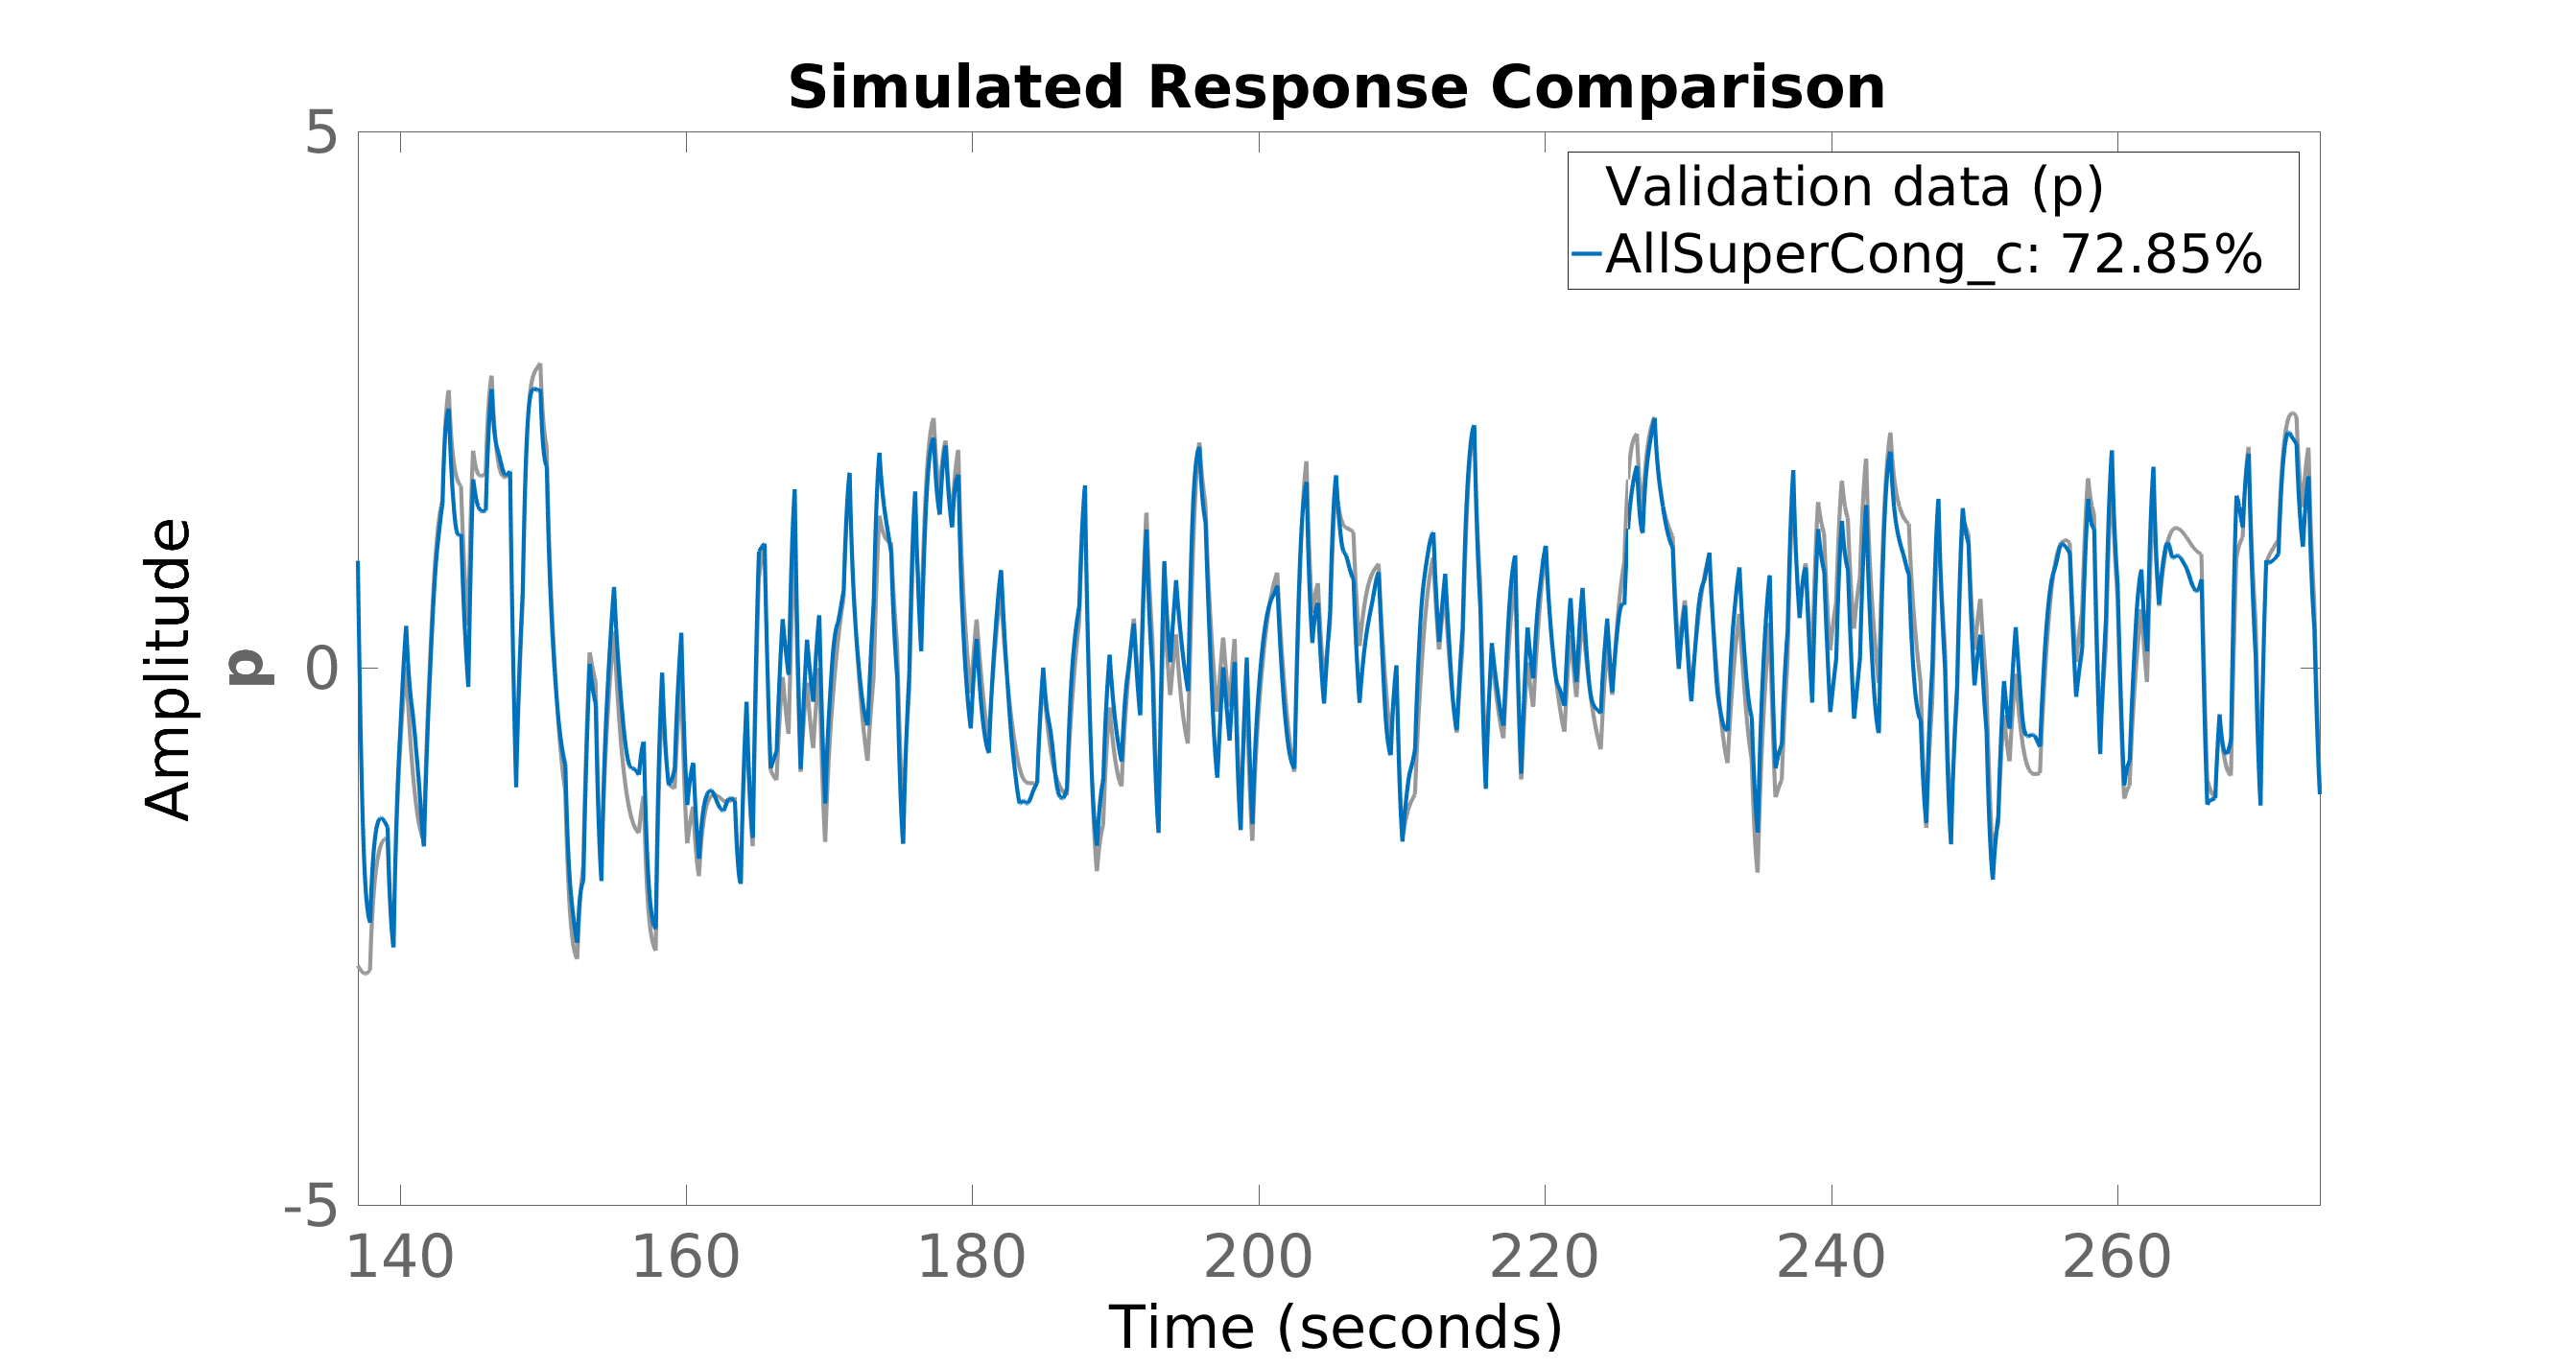
\includegraphics[width=0.4\textwidth]{angVelSimp}}
  \qquad
  \subfloat[][\label{fig:angVelSimq}Angular velocity around the \abbrROV's y-axis.]{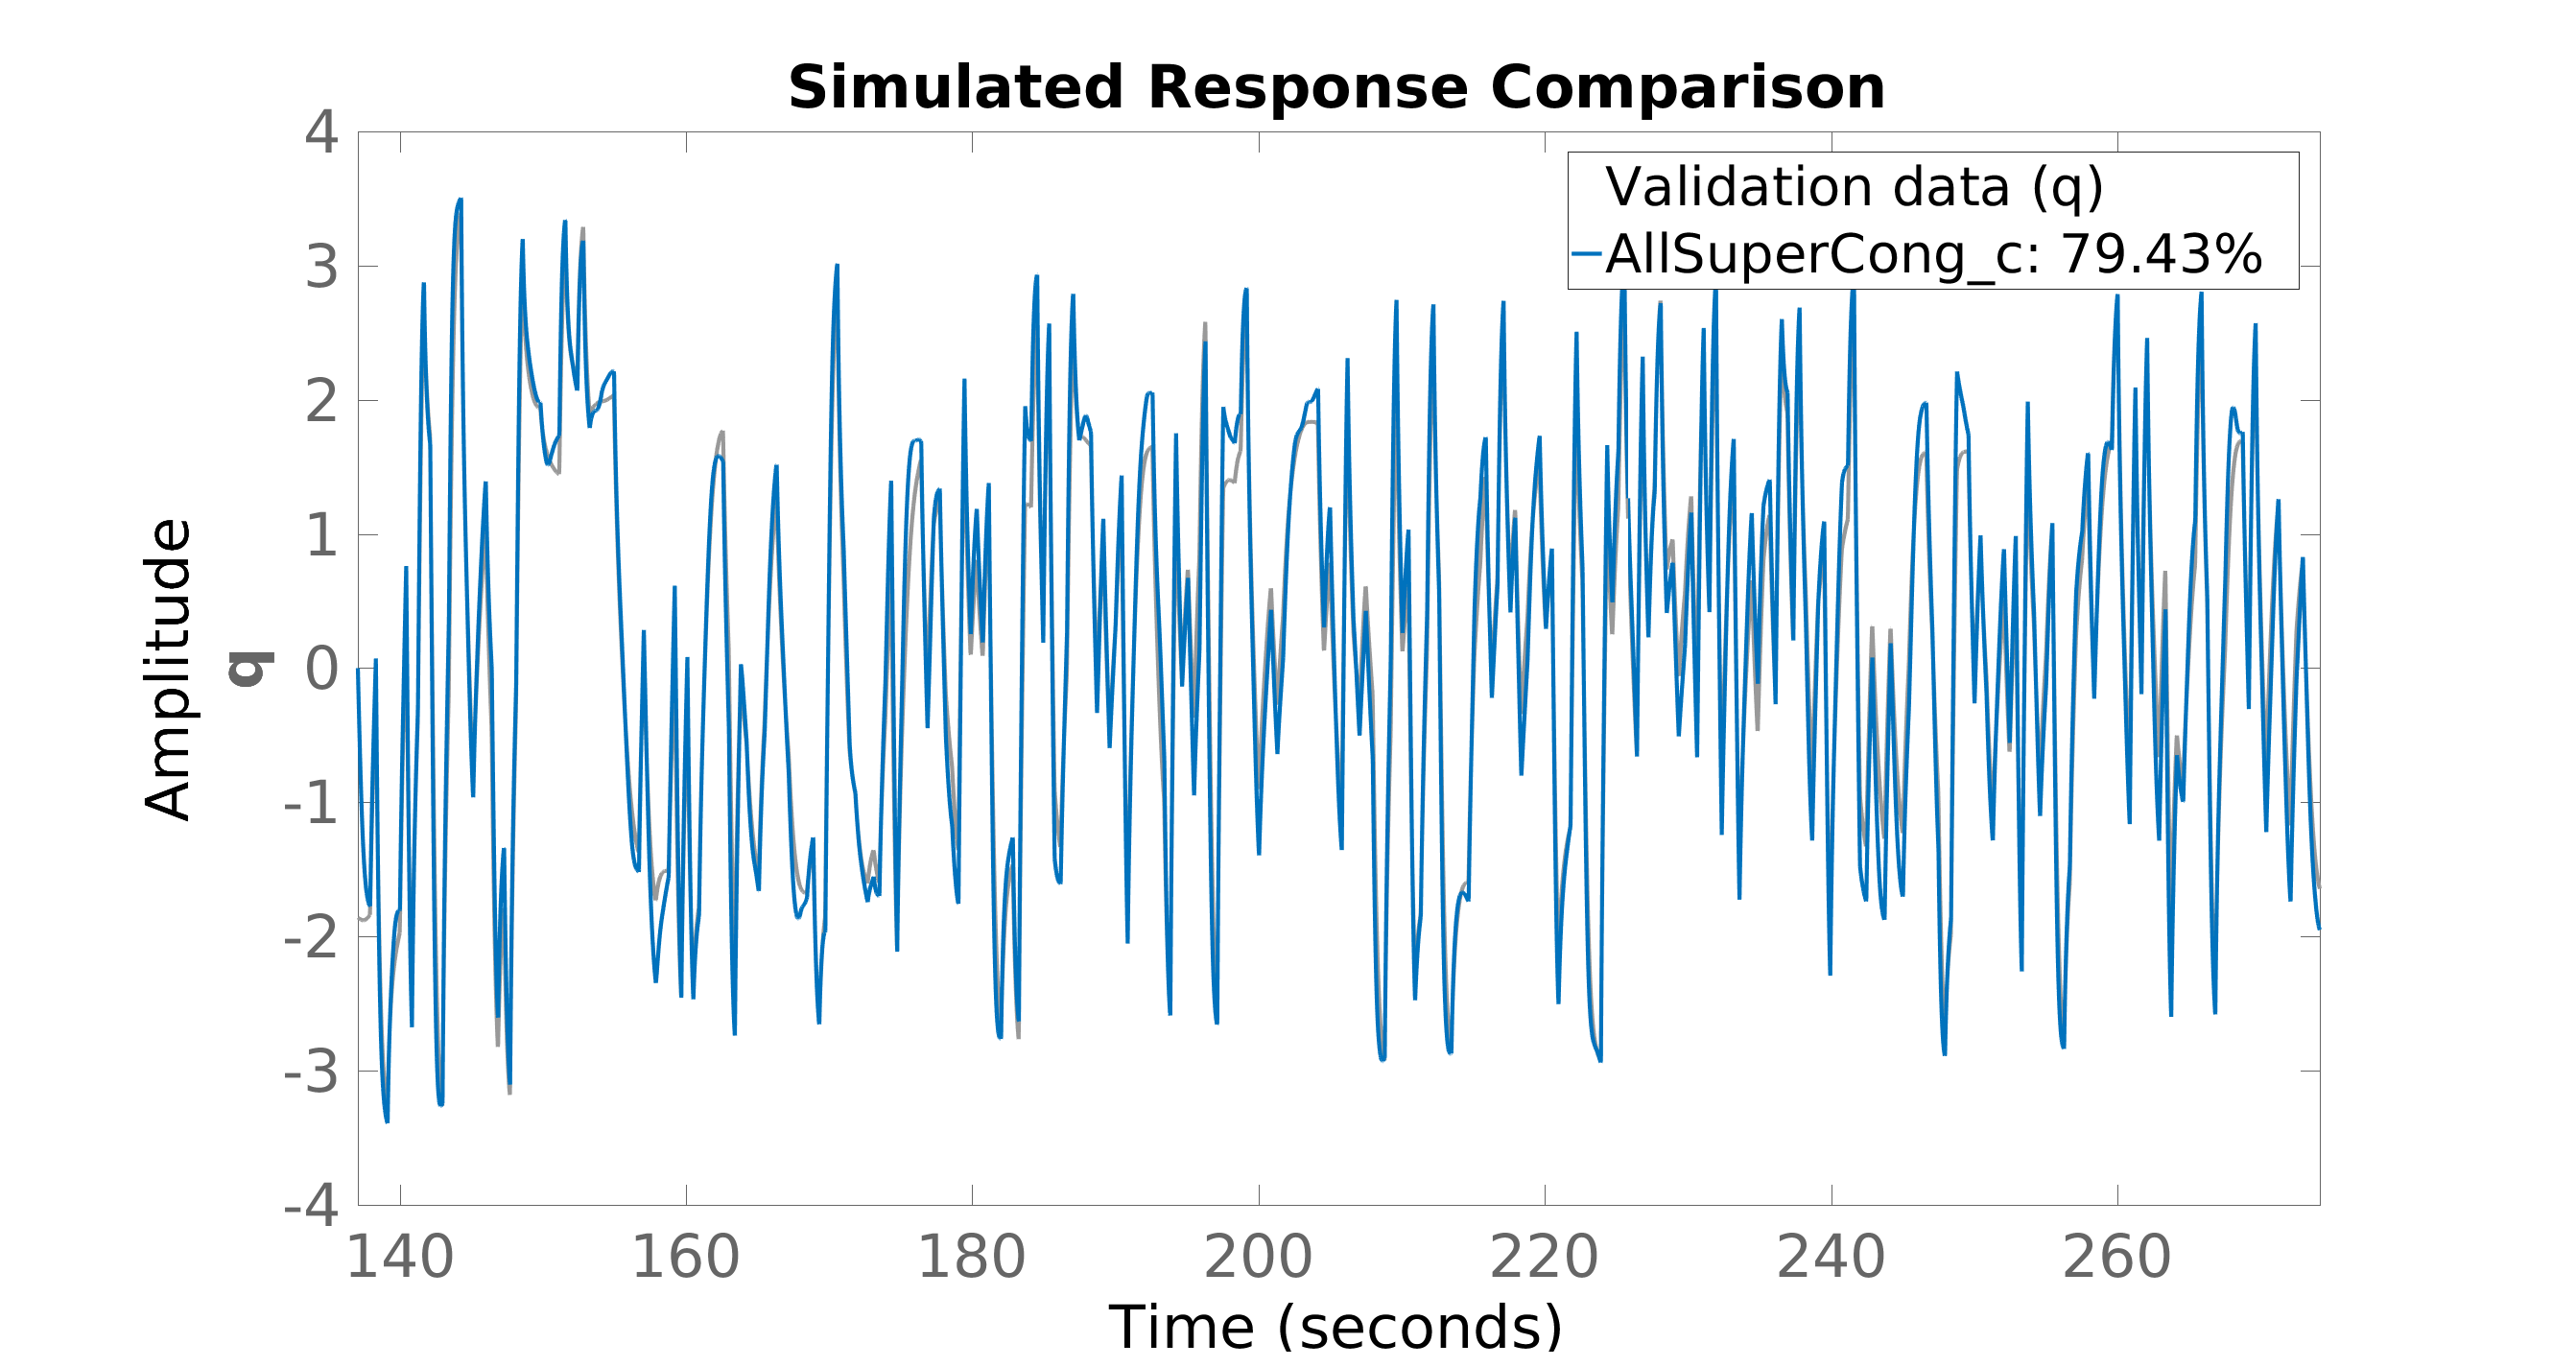
\includegraphics[width=0.4\textwidth]{angVelSimq}}
  \qquad
  \subfloat[][\label{fig:angVelSimr}Angular velocity around the \abbrROV's z-axis.]{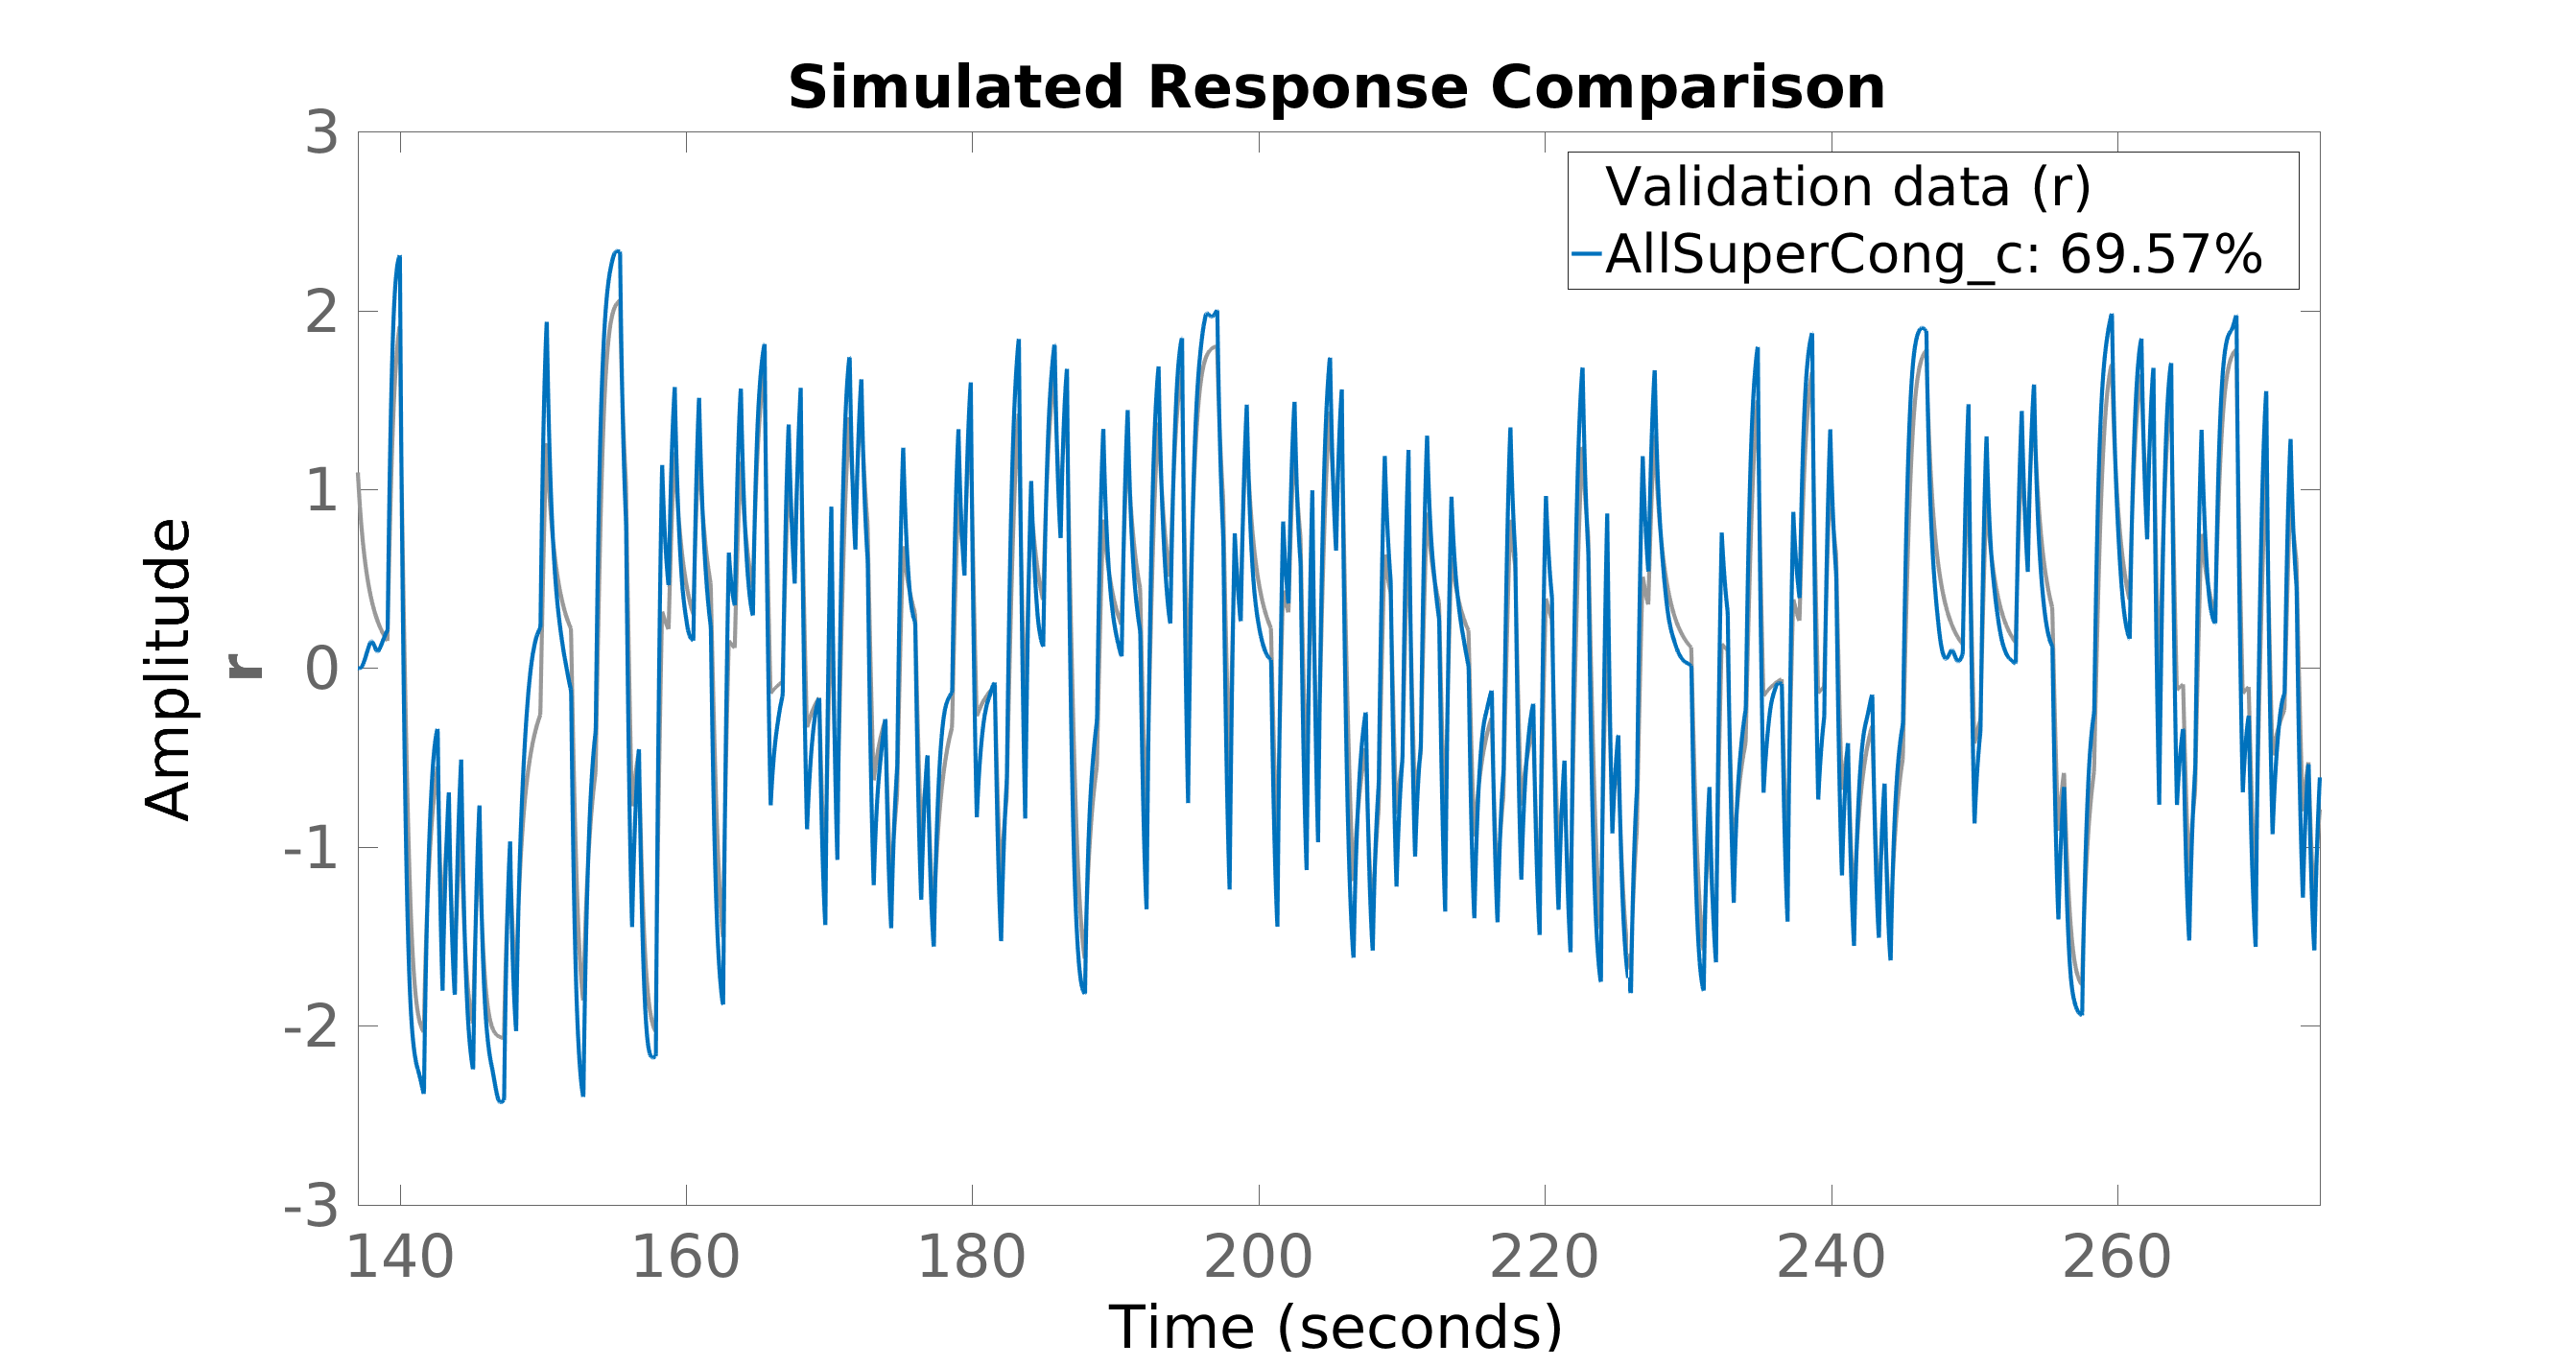
\includegraphics[width=0.4\textwidth]{angVelSimr}}
    \qquad
  \subfloat[][\label{fig:linAccSimx}Linear acceleration in the \abbrROV's x-axis.]{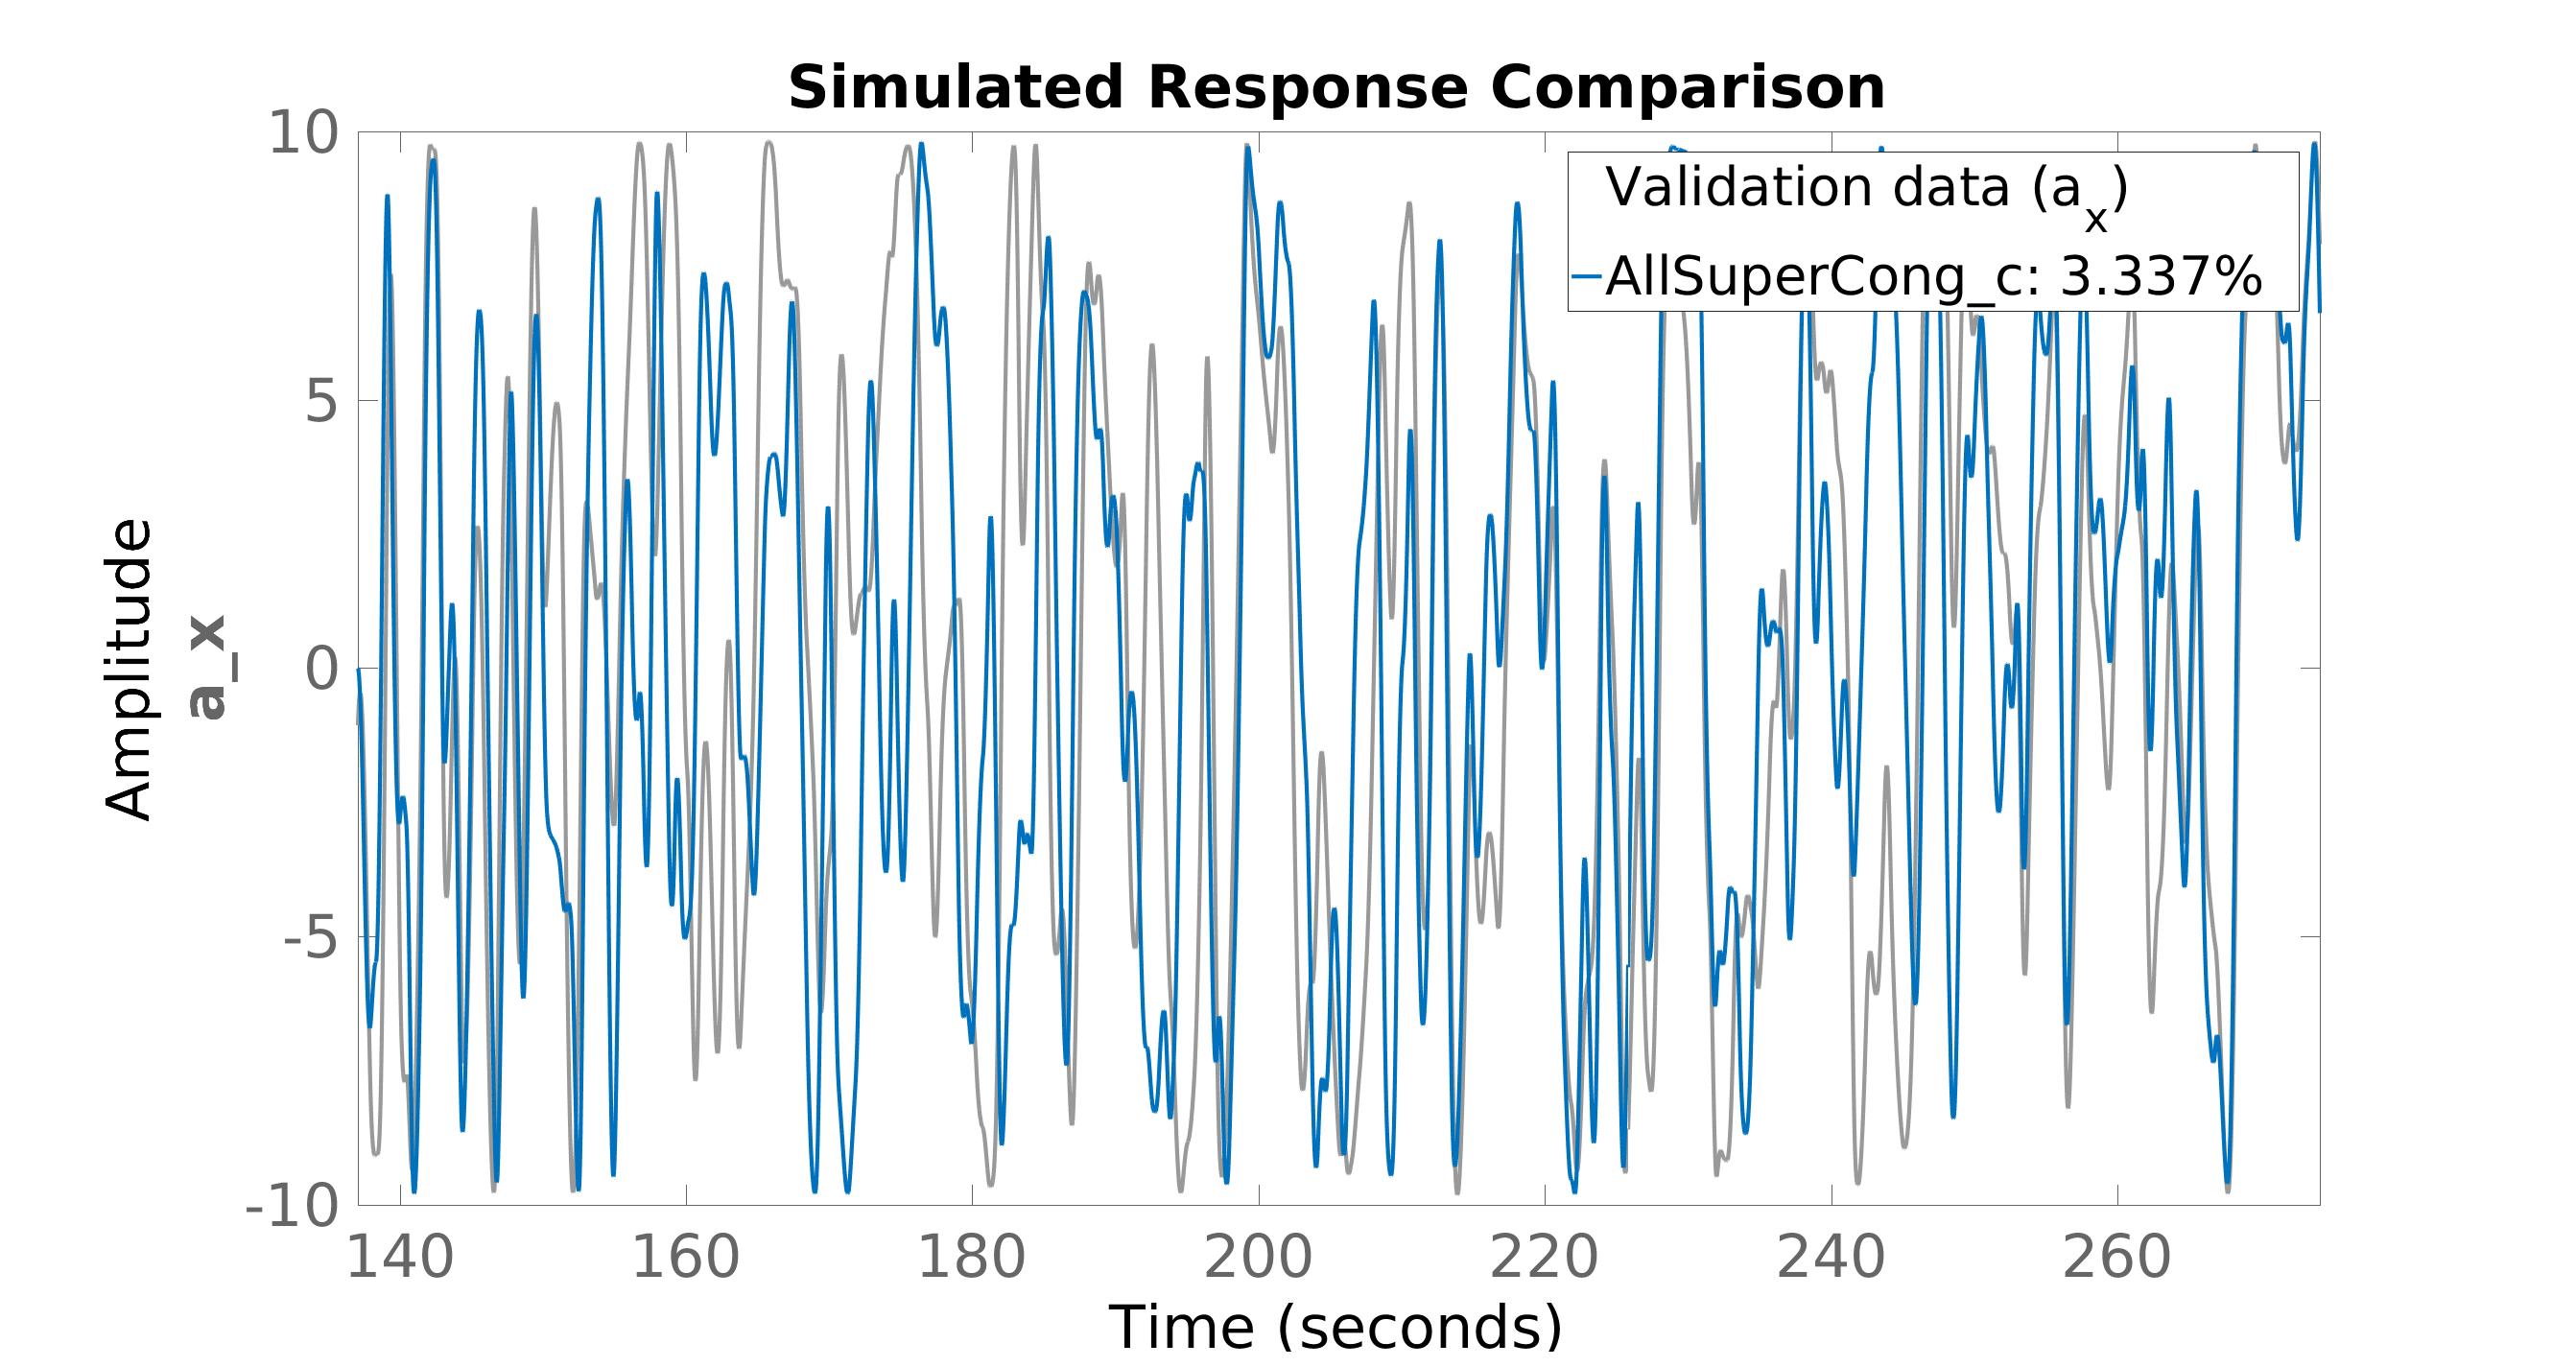
\includegraphics[width=0.4\textwidth]{linAccSimx}}
    \qquad
  \subfloat[][\label{fig:linAccSimy}Linear acceleration in the \abbrROV's y-axis.]{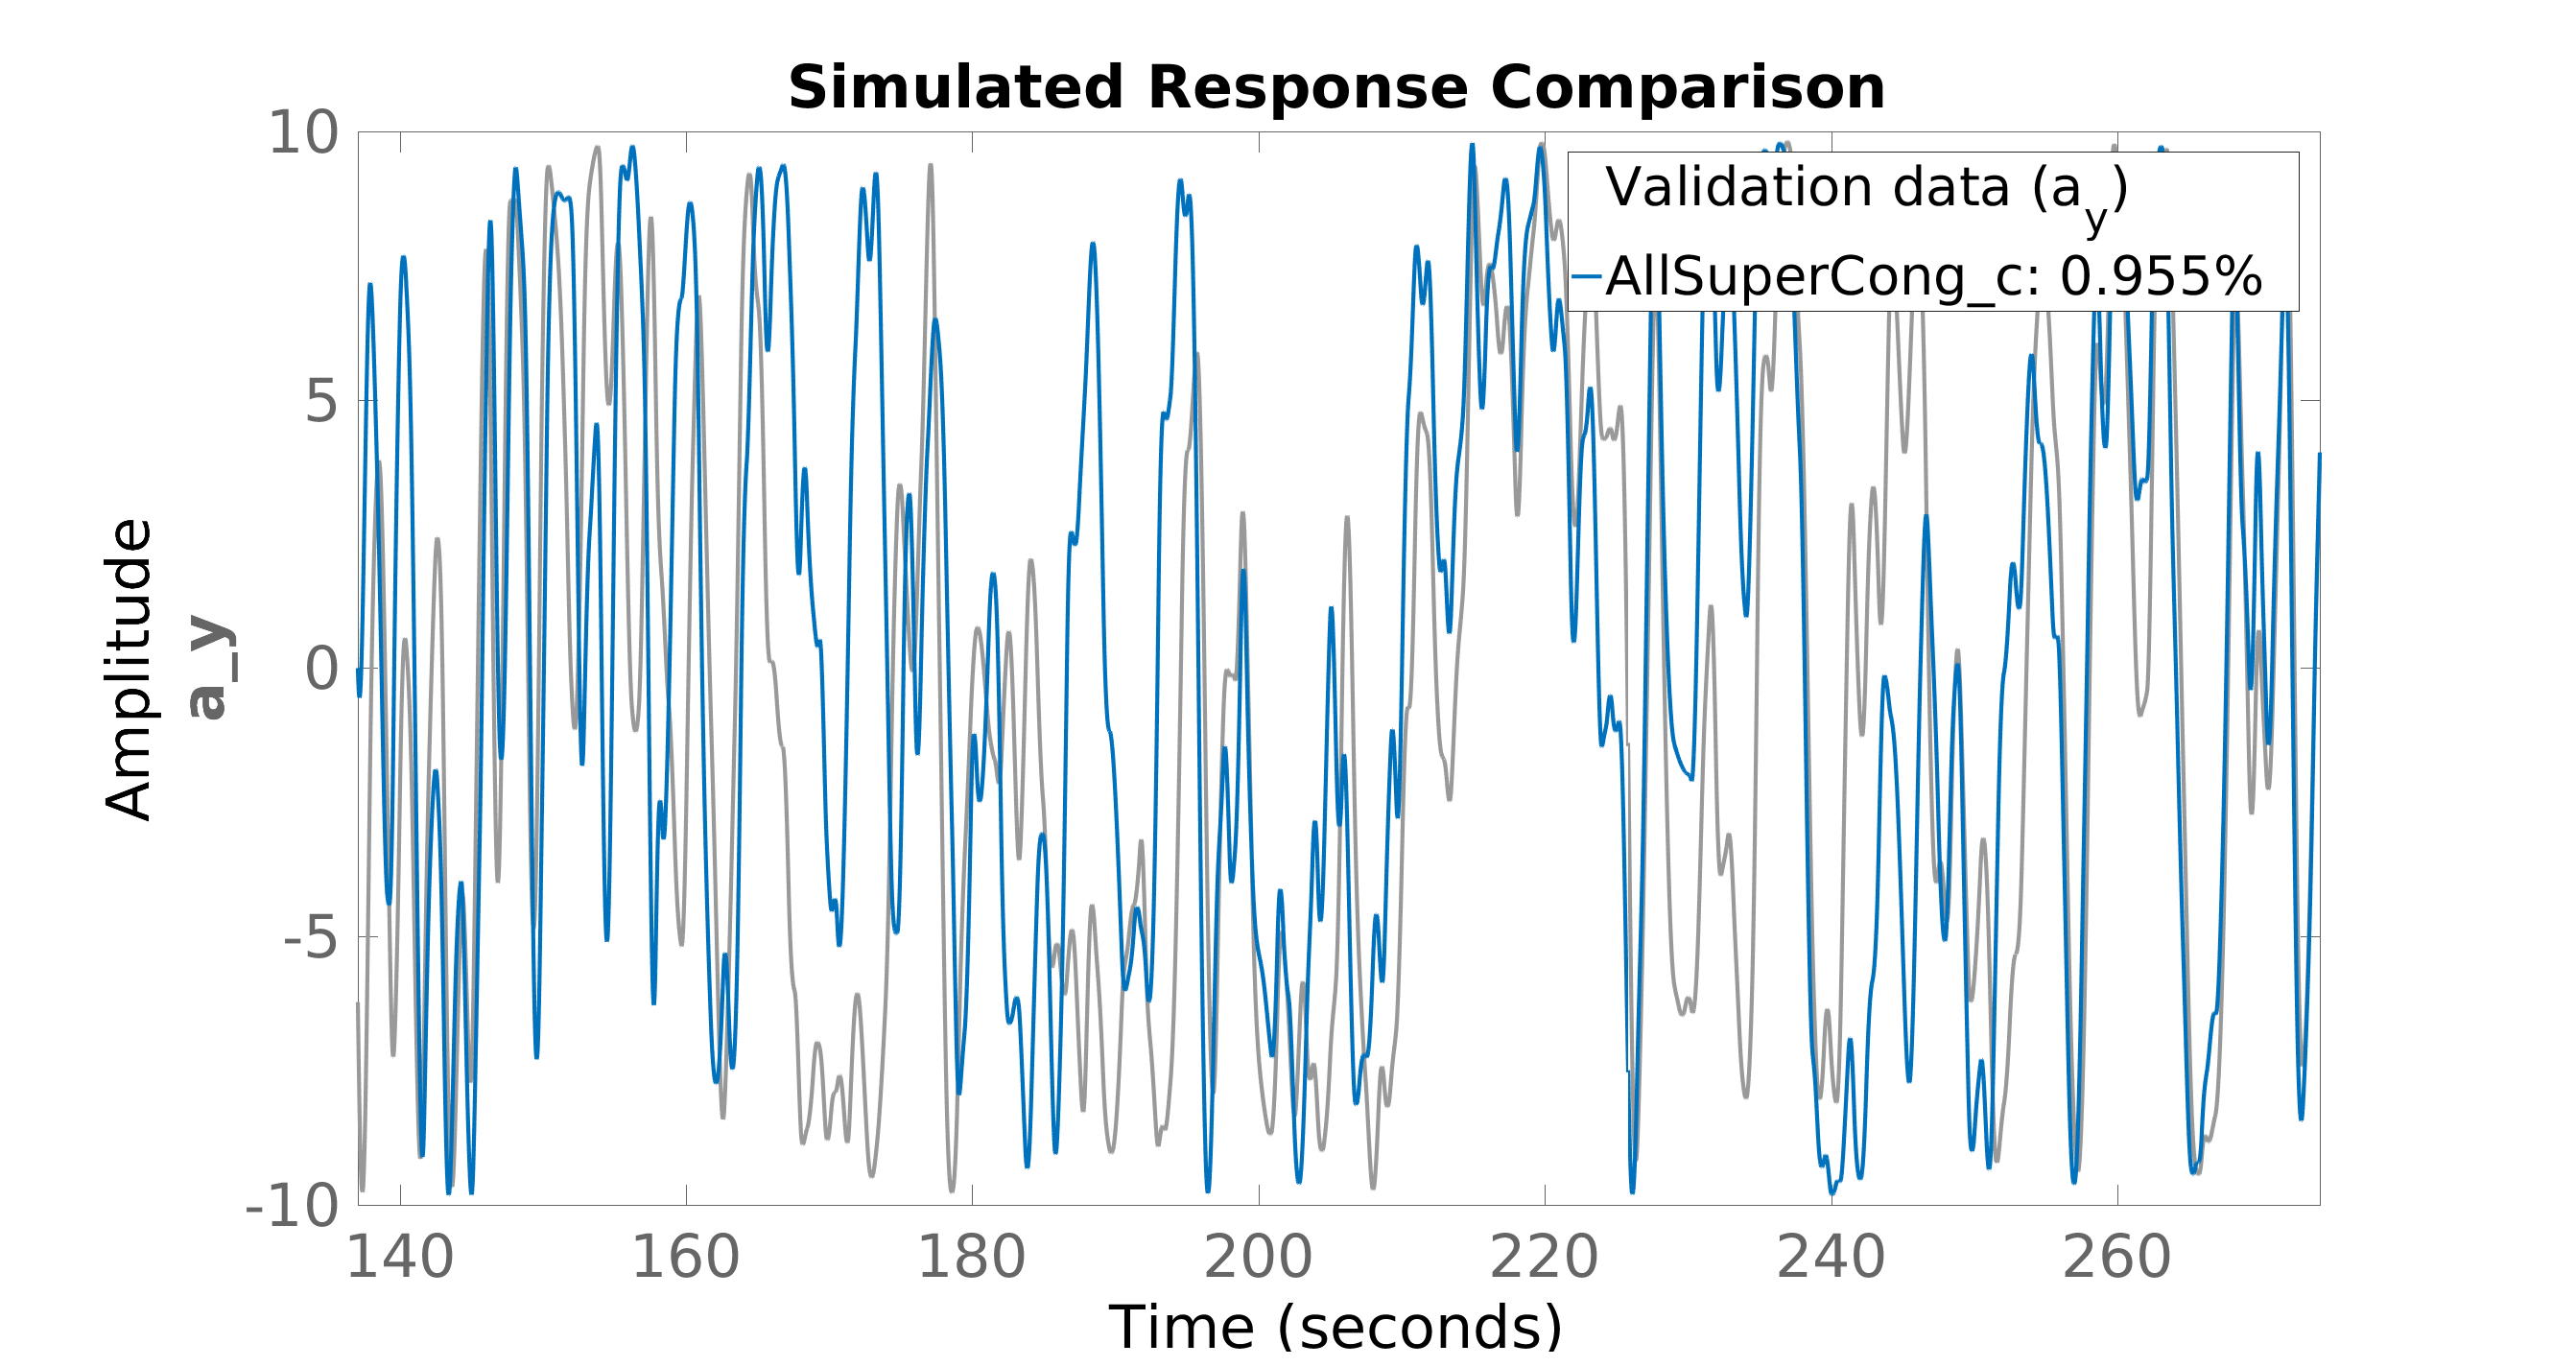
\includegraphics[width=0.4\textwidth]{linAccSimy}}
    \qquad
  \subfloat[][\label{fig:linAccSimz}Linear acceleration  in the \abbrROV's z-axis.]{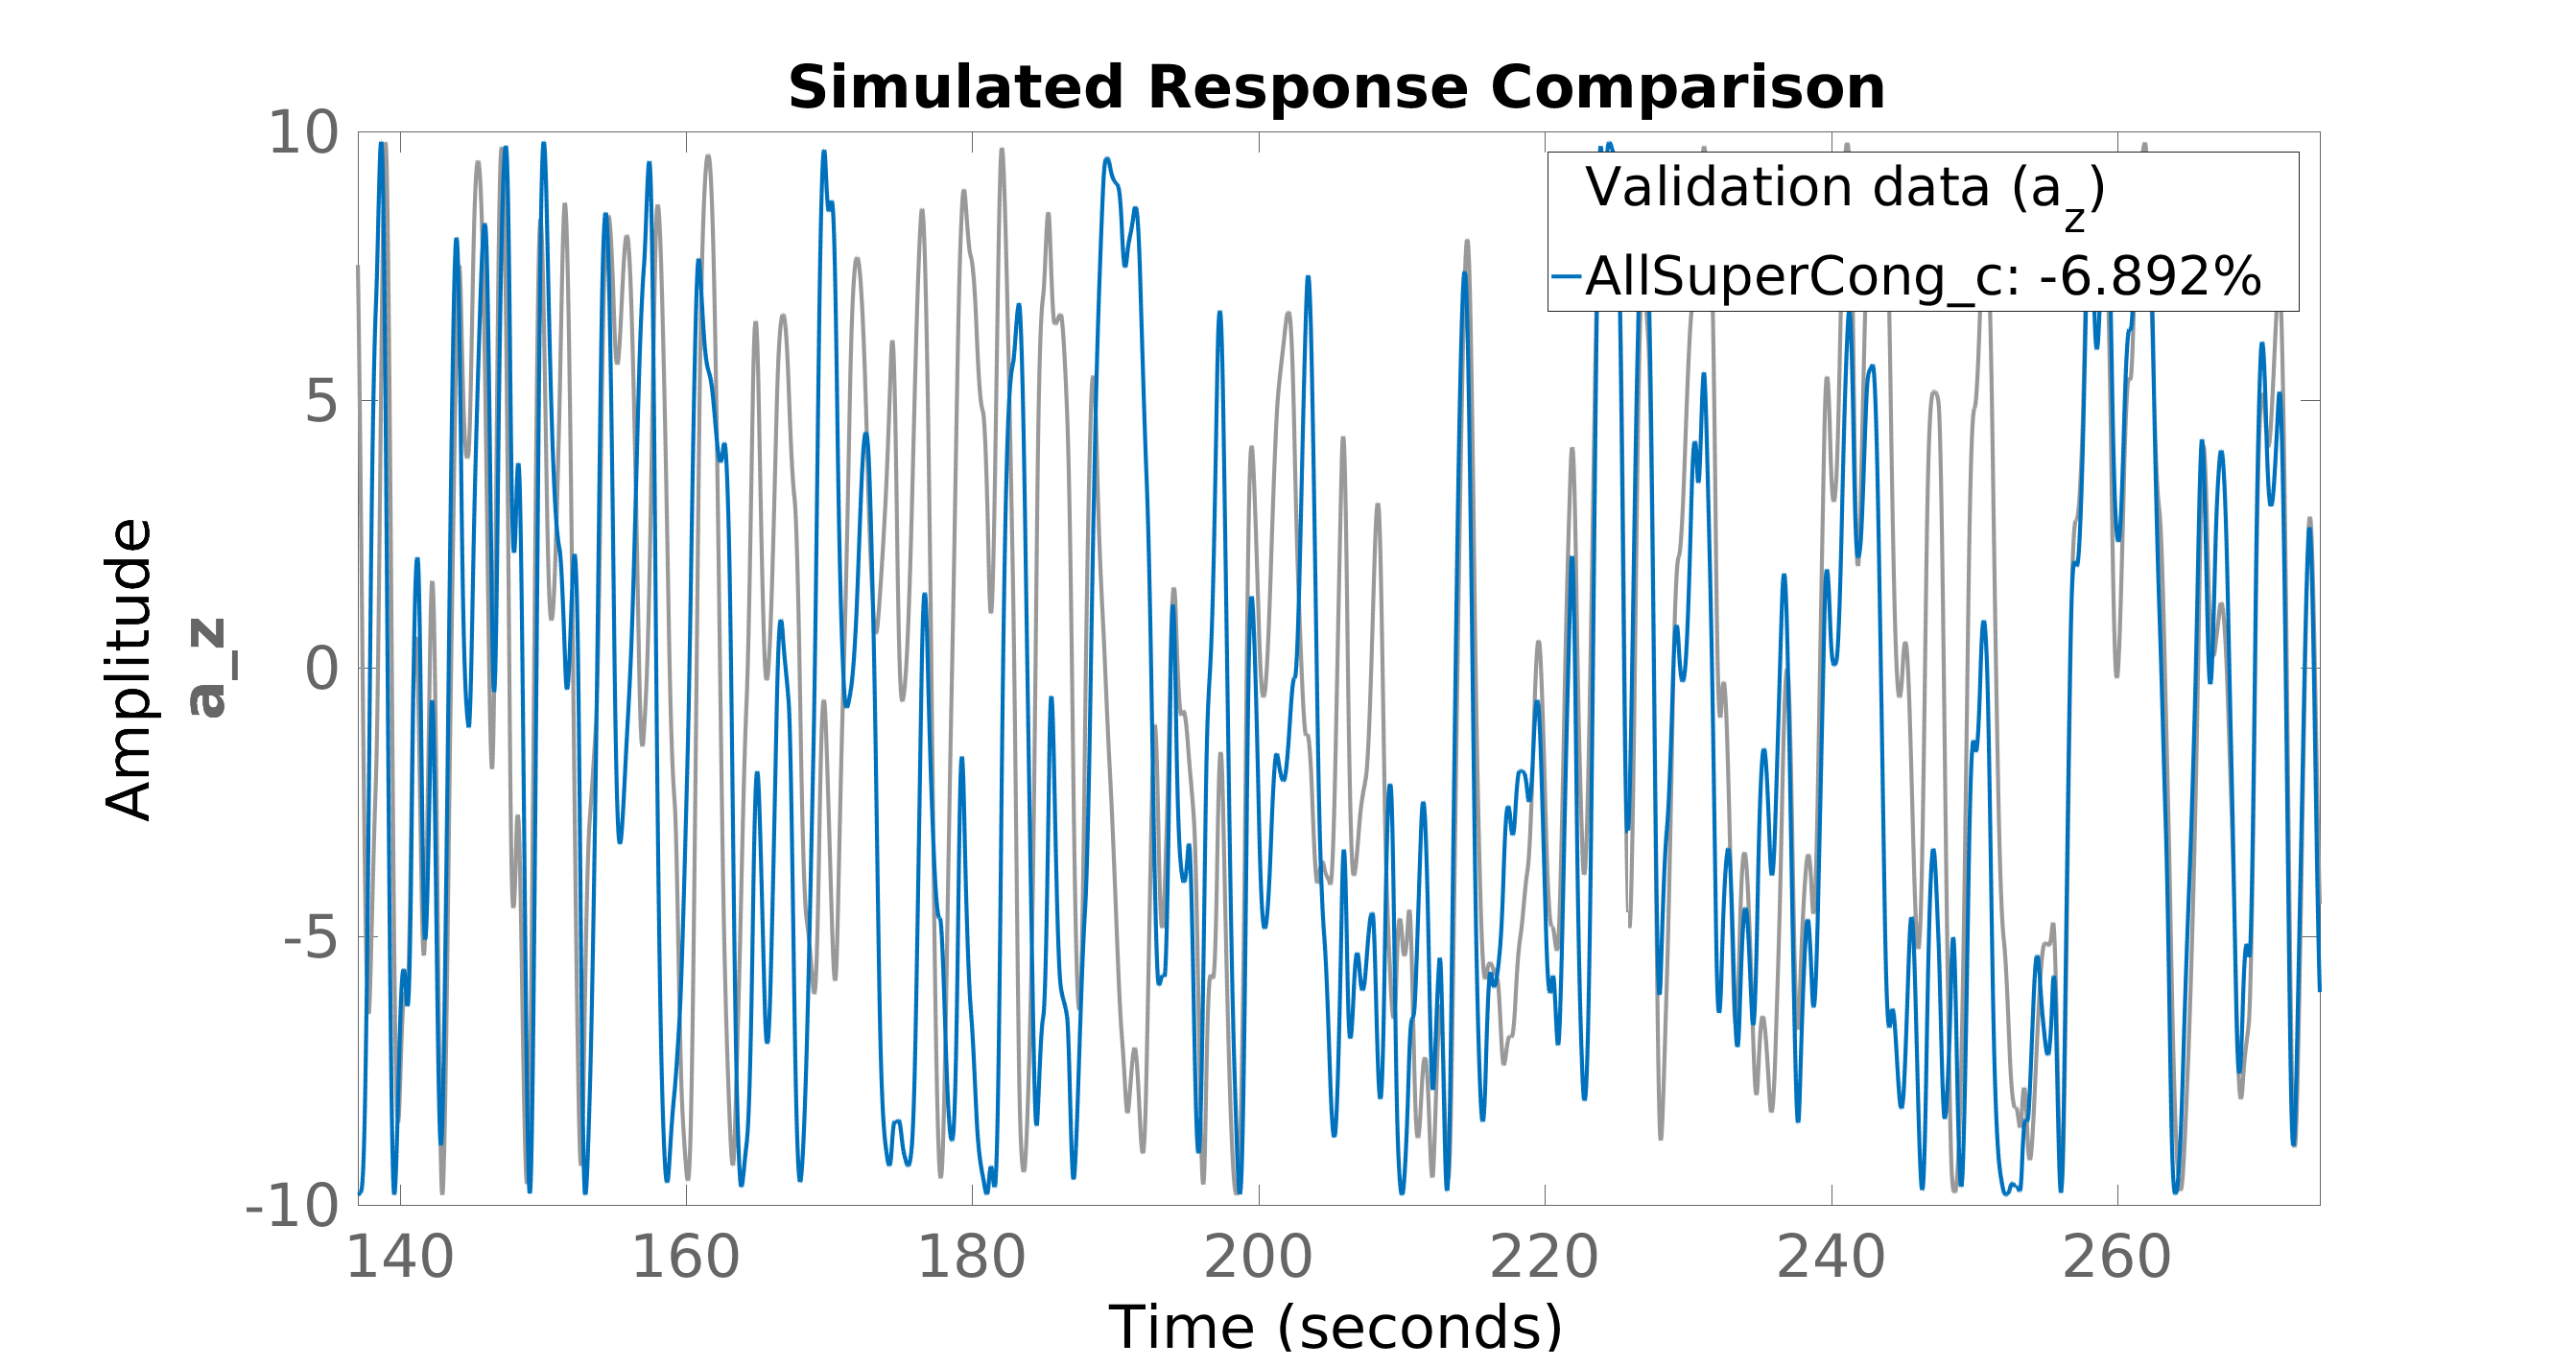
\includegraphics[width=0.4\textwidth]{linAccSimz}}
  \caption{\label{fig:angVelSim}%
    Comparison between simulated validation data (grey) and the simulated response from the estimated model (blue). The fit for the model in each state is stated in each plot. The validation data has been generated using the initial parameters used in the parameter estimation. The poor initial state estimate results in that the estimated parameters diverge from their true values.}
\end{figure}

To estimate the initial state of the quaternions, a Kalman smoother as described in \citet{Wallin} was used. The magnetometer was also added as an output, in the Kalman smoother, to further reduce the uncertainty of the initial quaternions. It is therefore recommended that attitude data is logged on quaternion form so that the initial quaternions can easily be obtained during parameter estimation. An alternative is that the \abbrROV's initial attitude is known. 

The estimated parameter values obtained when using \eqref{eq:quatModel} with angular velocities and linear accelerations as inputs can be seen in \Tableref{tab:ResultEstimAngular}. The fit of the model using the estimated parameters can be seen in \Figureref{fig:angVelComparelz6}. The high fit of $50\ \%$ in $q$ and $r$ means that the model describes parts of the validation data well. The model did not describe the linear accelerations and $p$ well, which can be seen in the low fit.

\begin{figure}[tbp]
  \centering
  \subfloat[][\label{fig:angVelCompareplz6}Angular velocity around the \abbrROV's x-axis.]{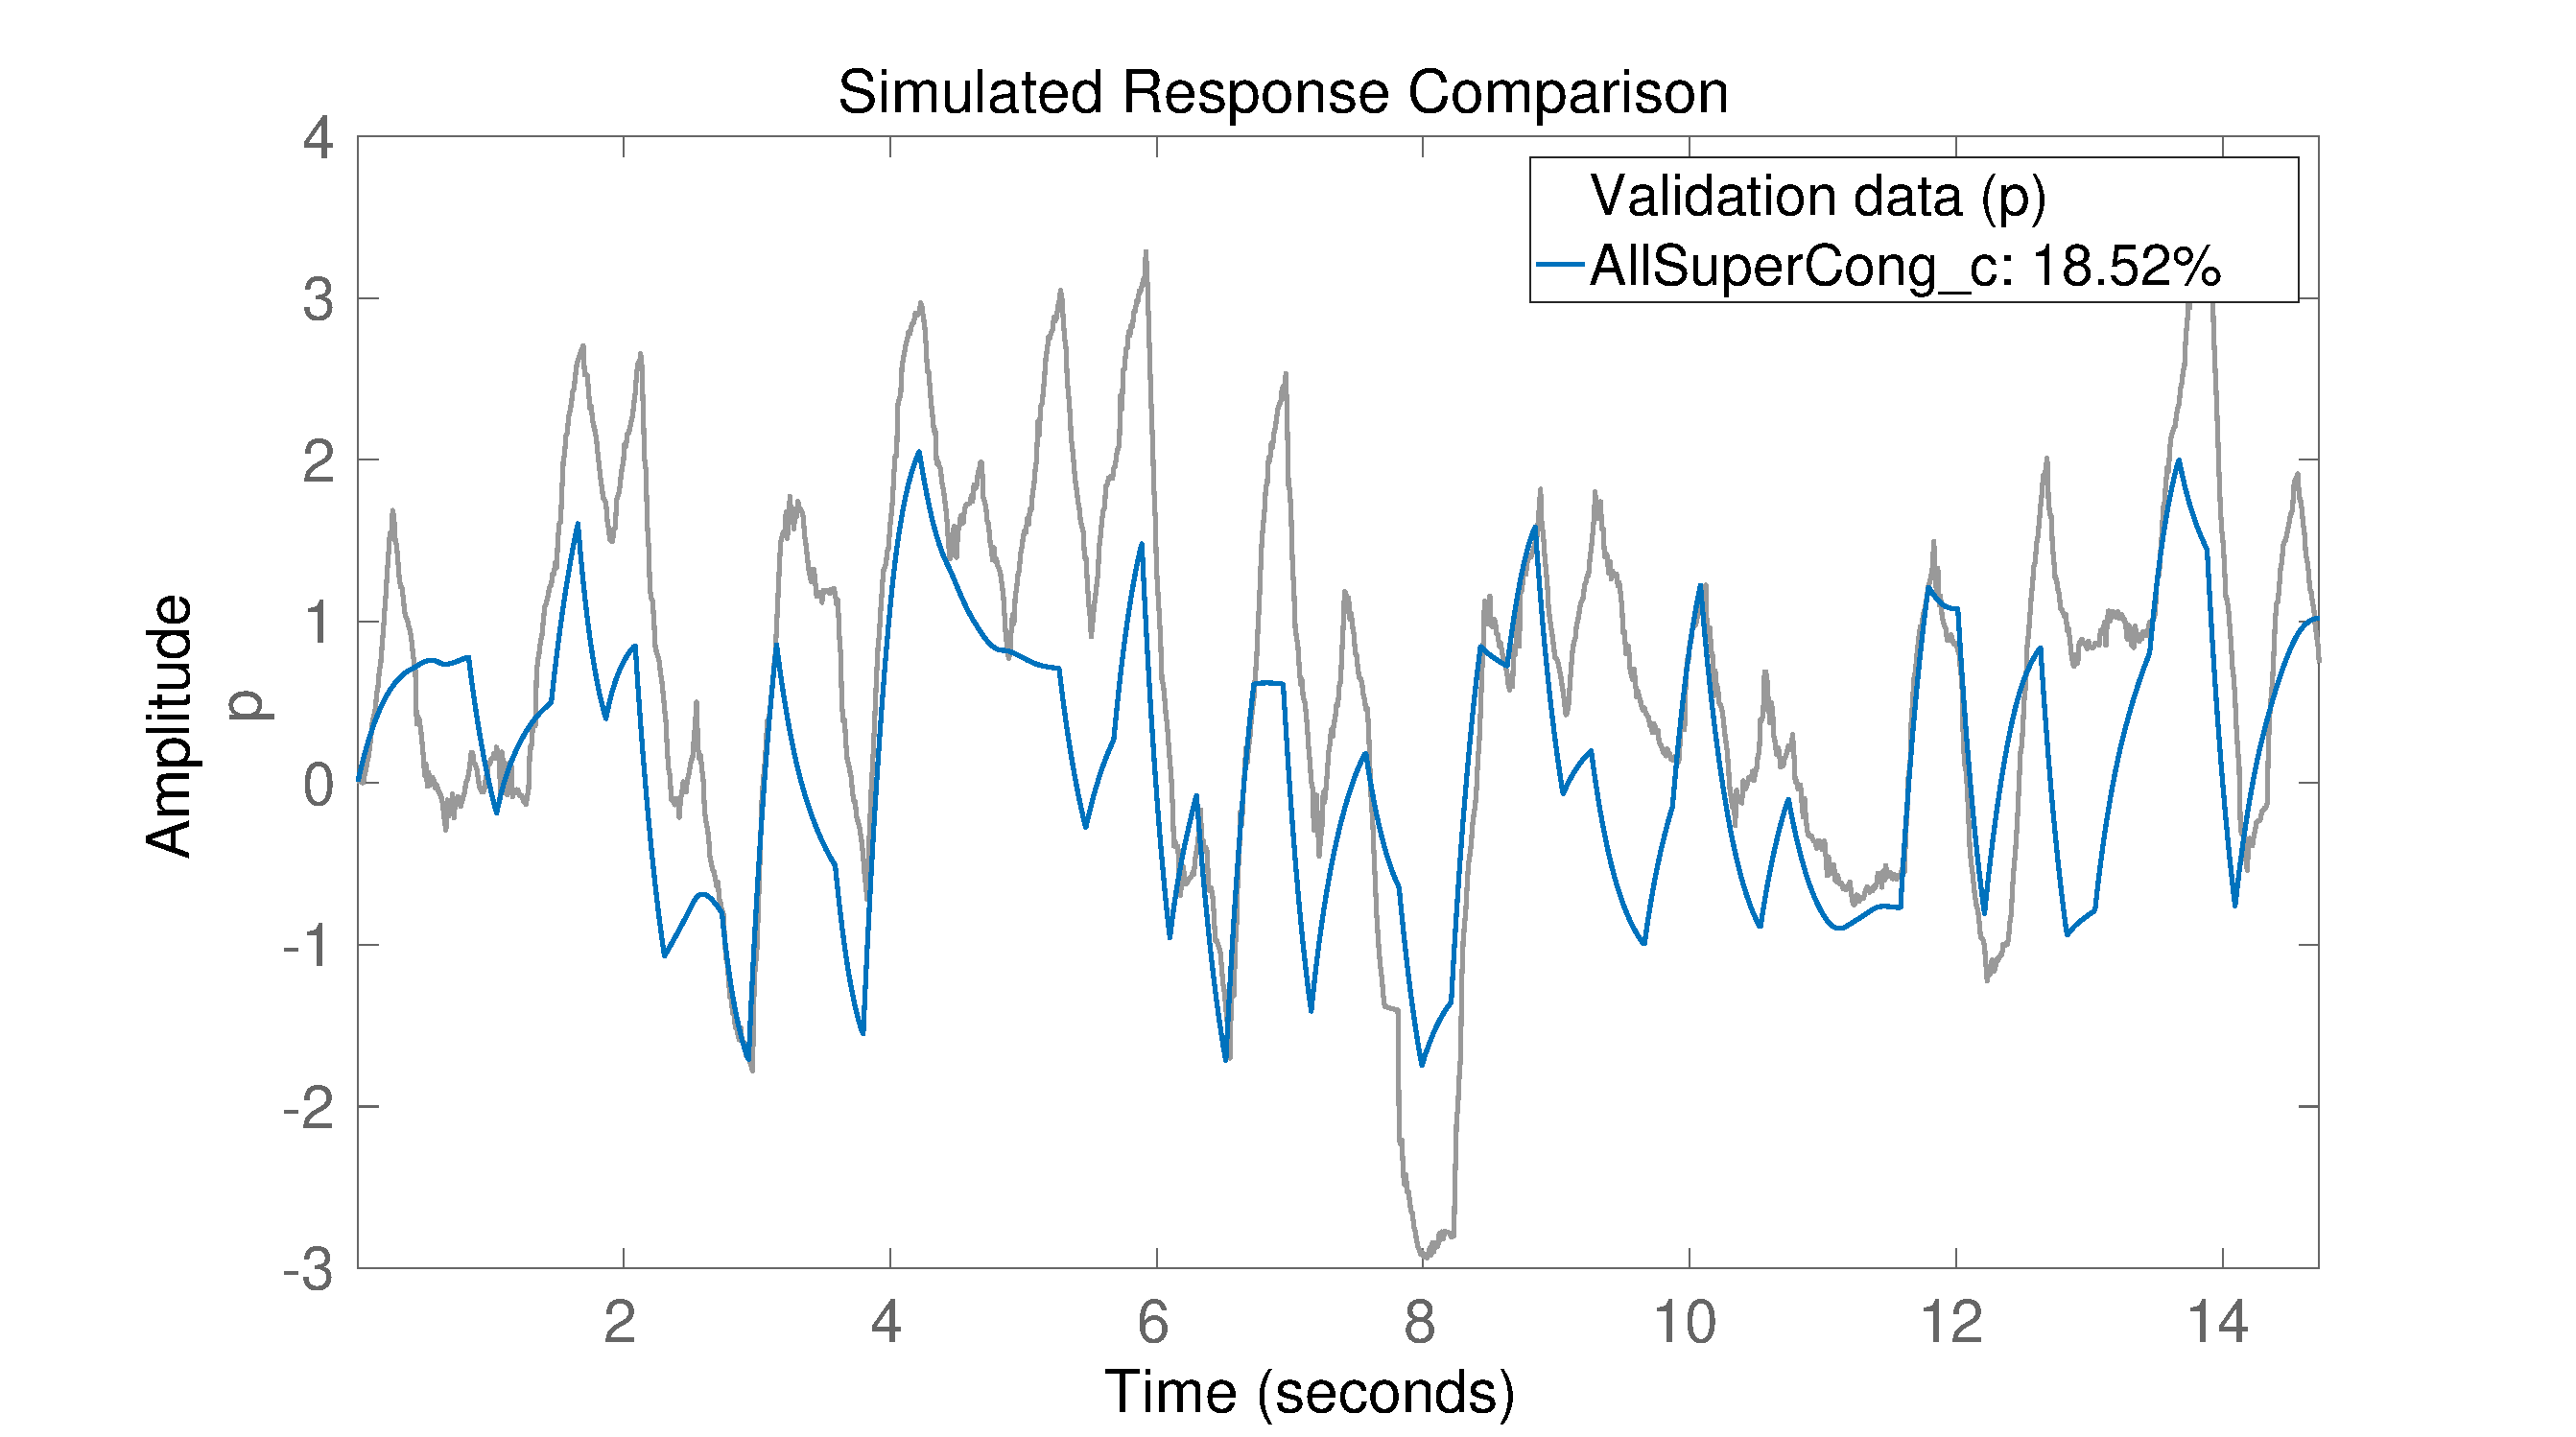
\includegraphics[width=0.4\textwidth]{angVelCompareplz6}}
  \qquad
  \subfloat[][\label{fig:angVelCompareqlz6}Angular velocity around the \abbrROV's y-axis.]{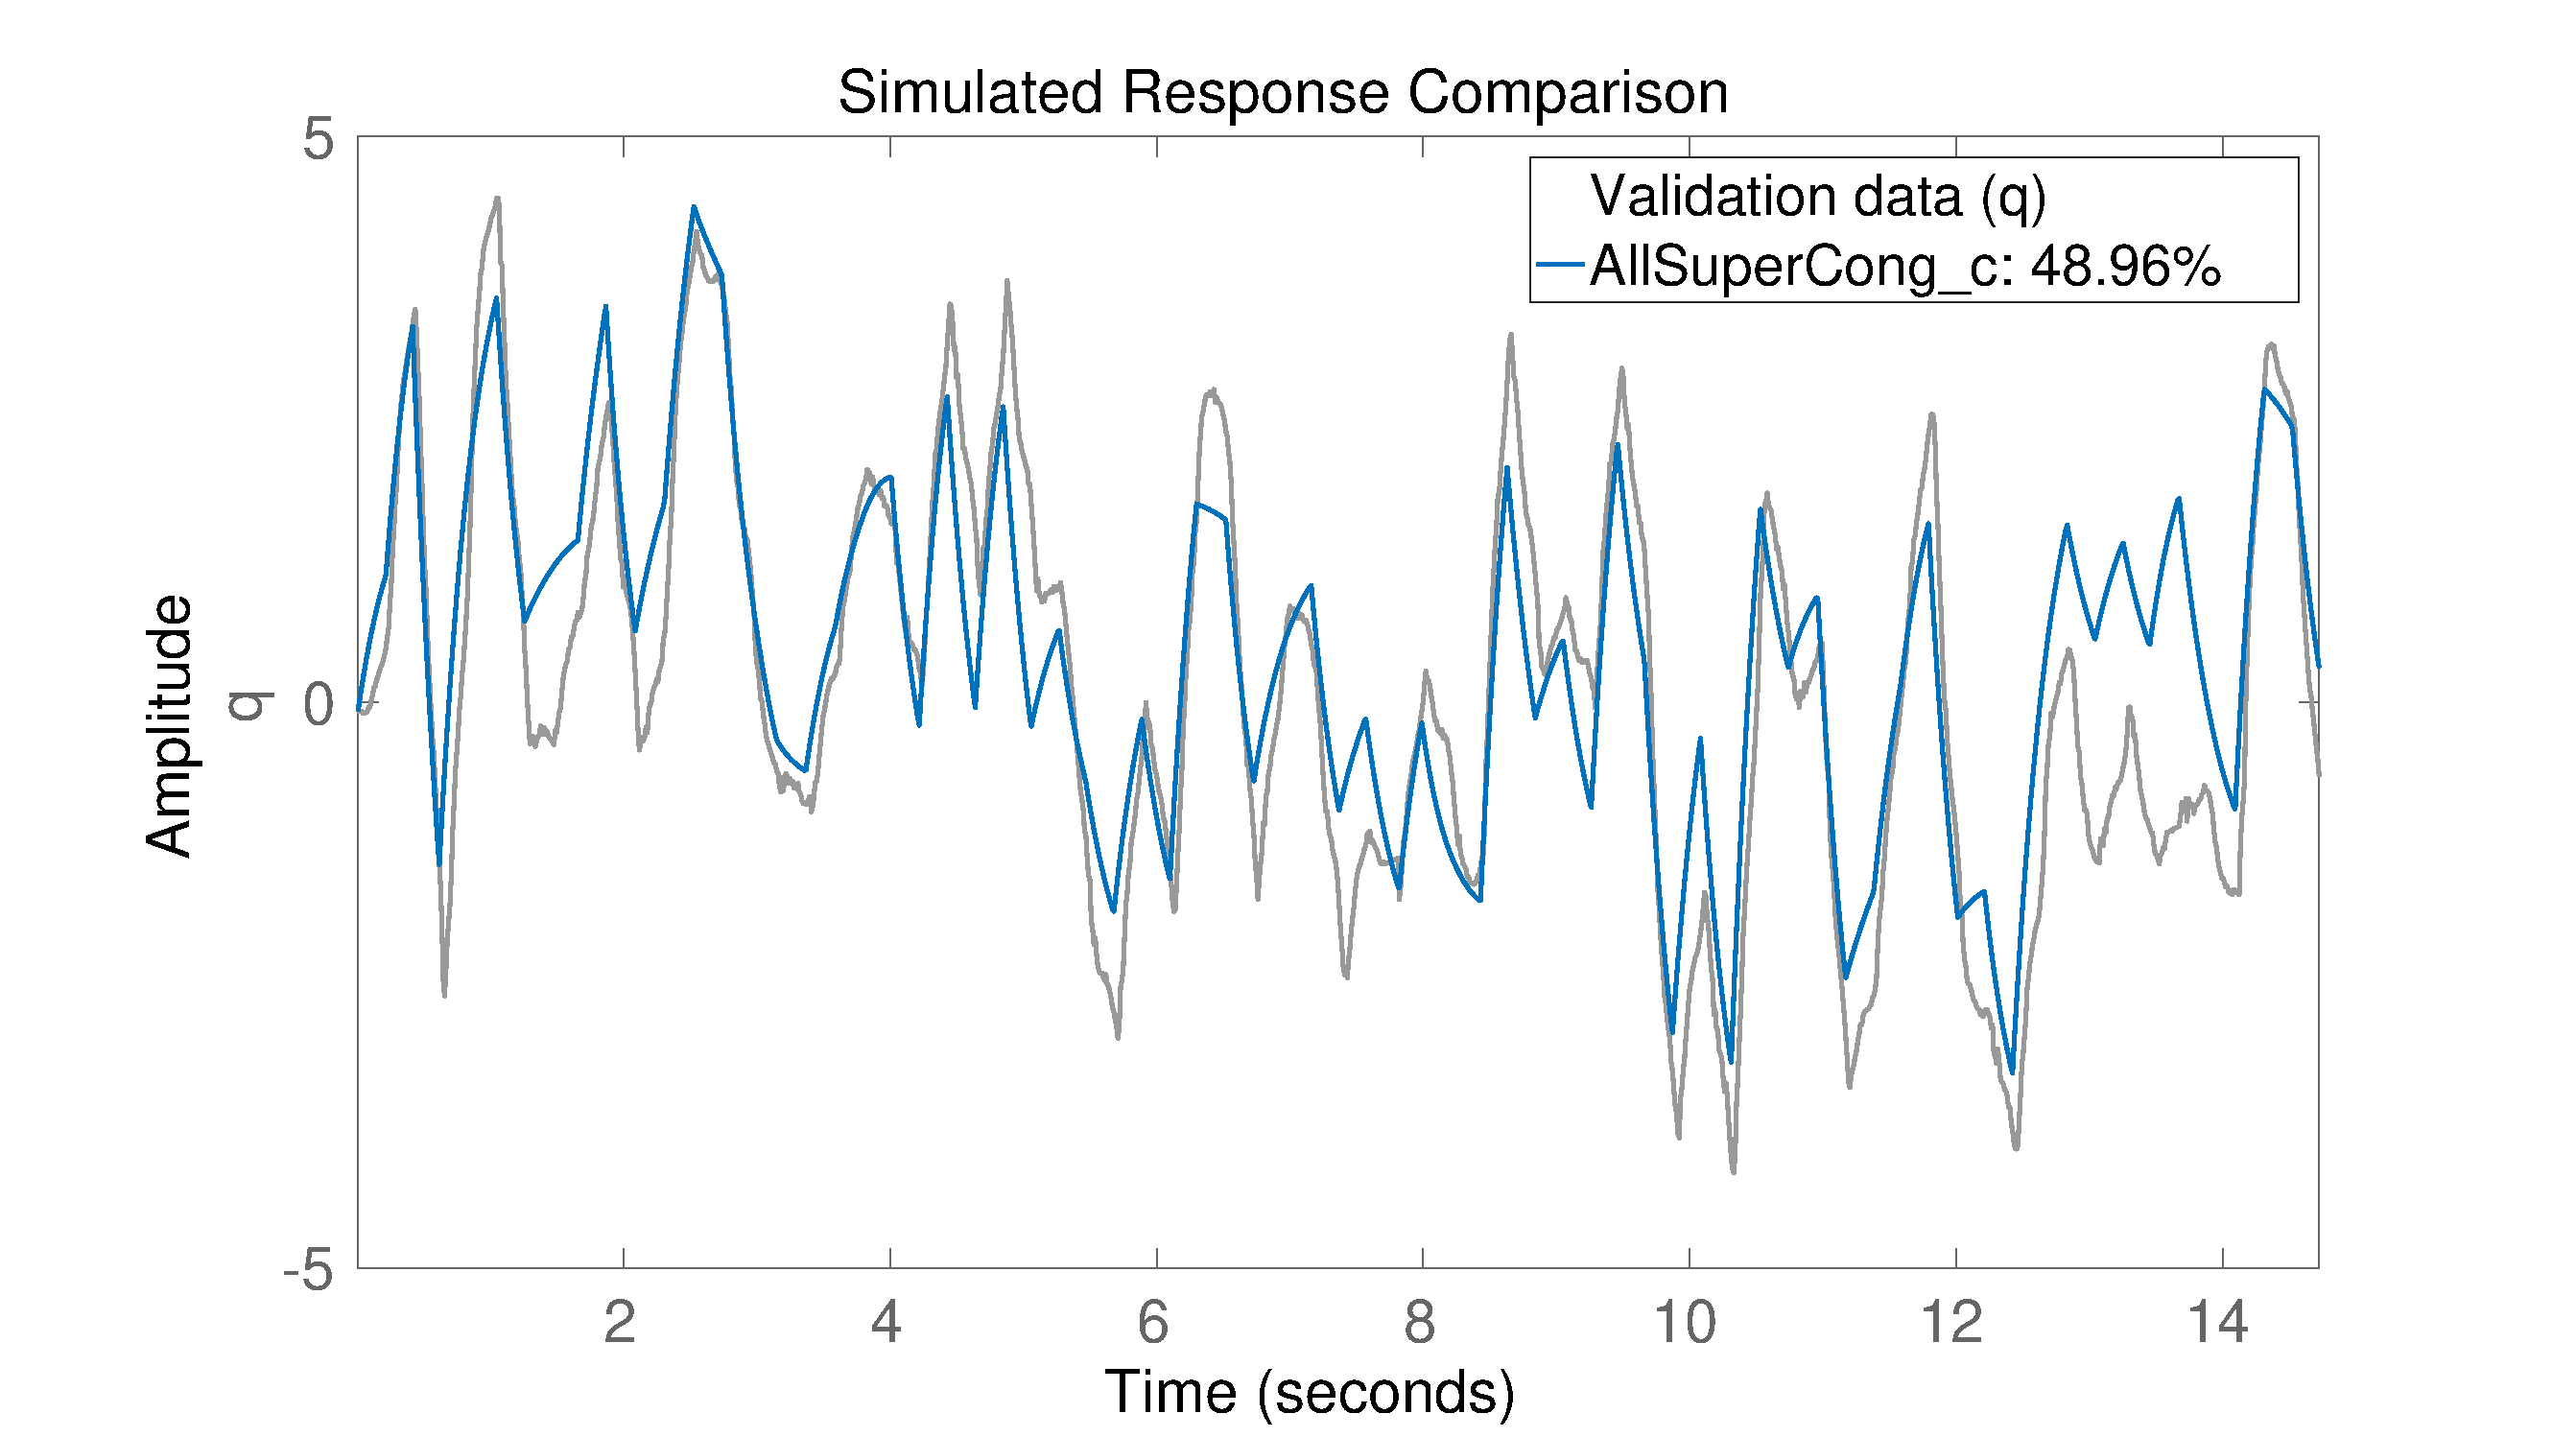
\includegraphics[width=0.4\textwidth]{angVelCompareqlz6}}
  \qquad
  \subfloat[][\label{fig:angVelComparerlz6}Angular velocity around the \abbrROV's z-axis.]{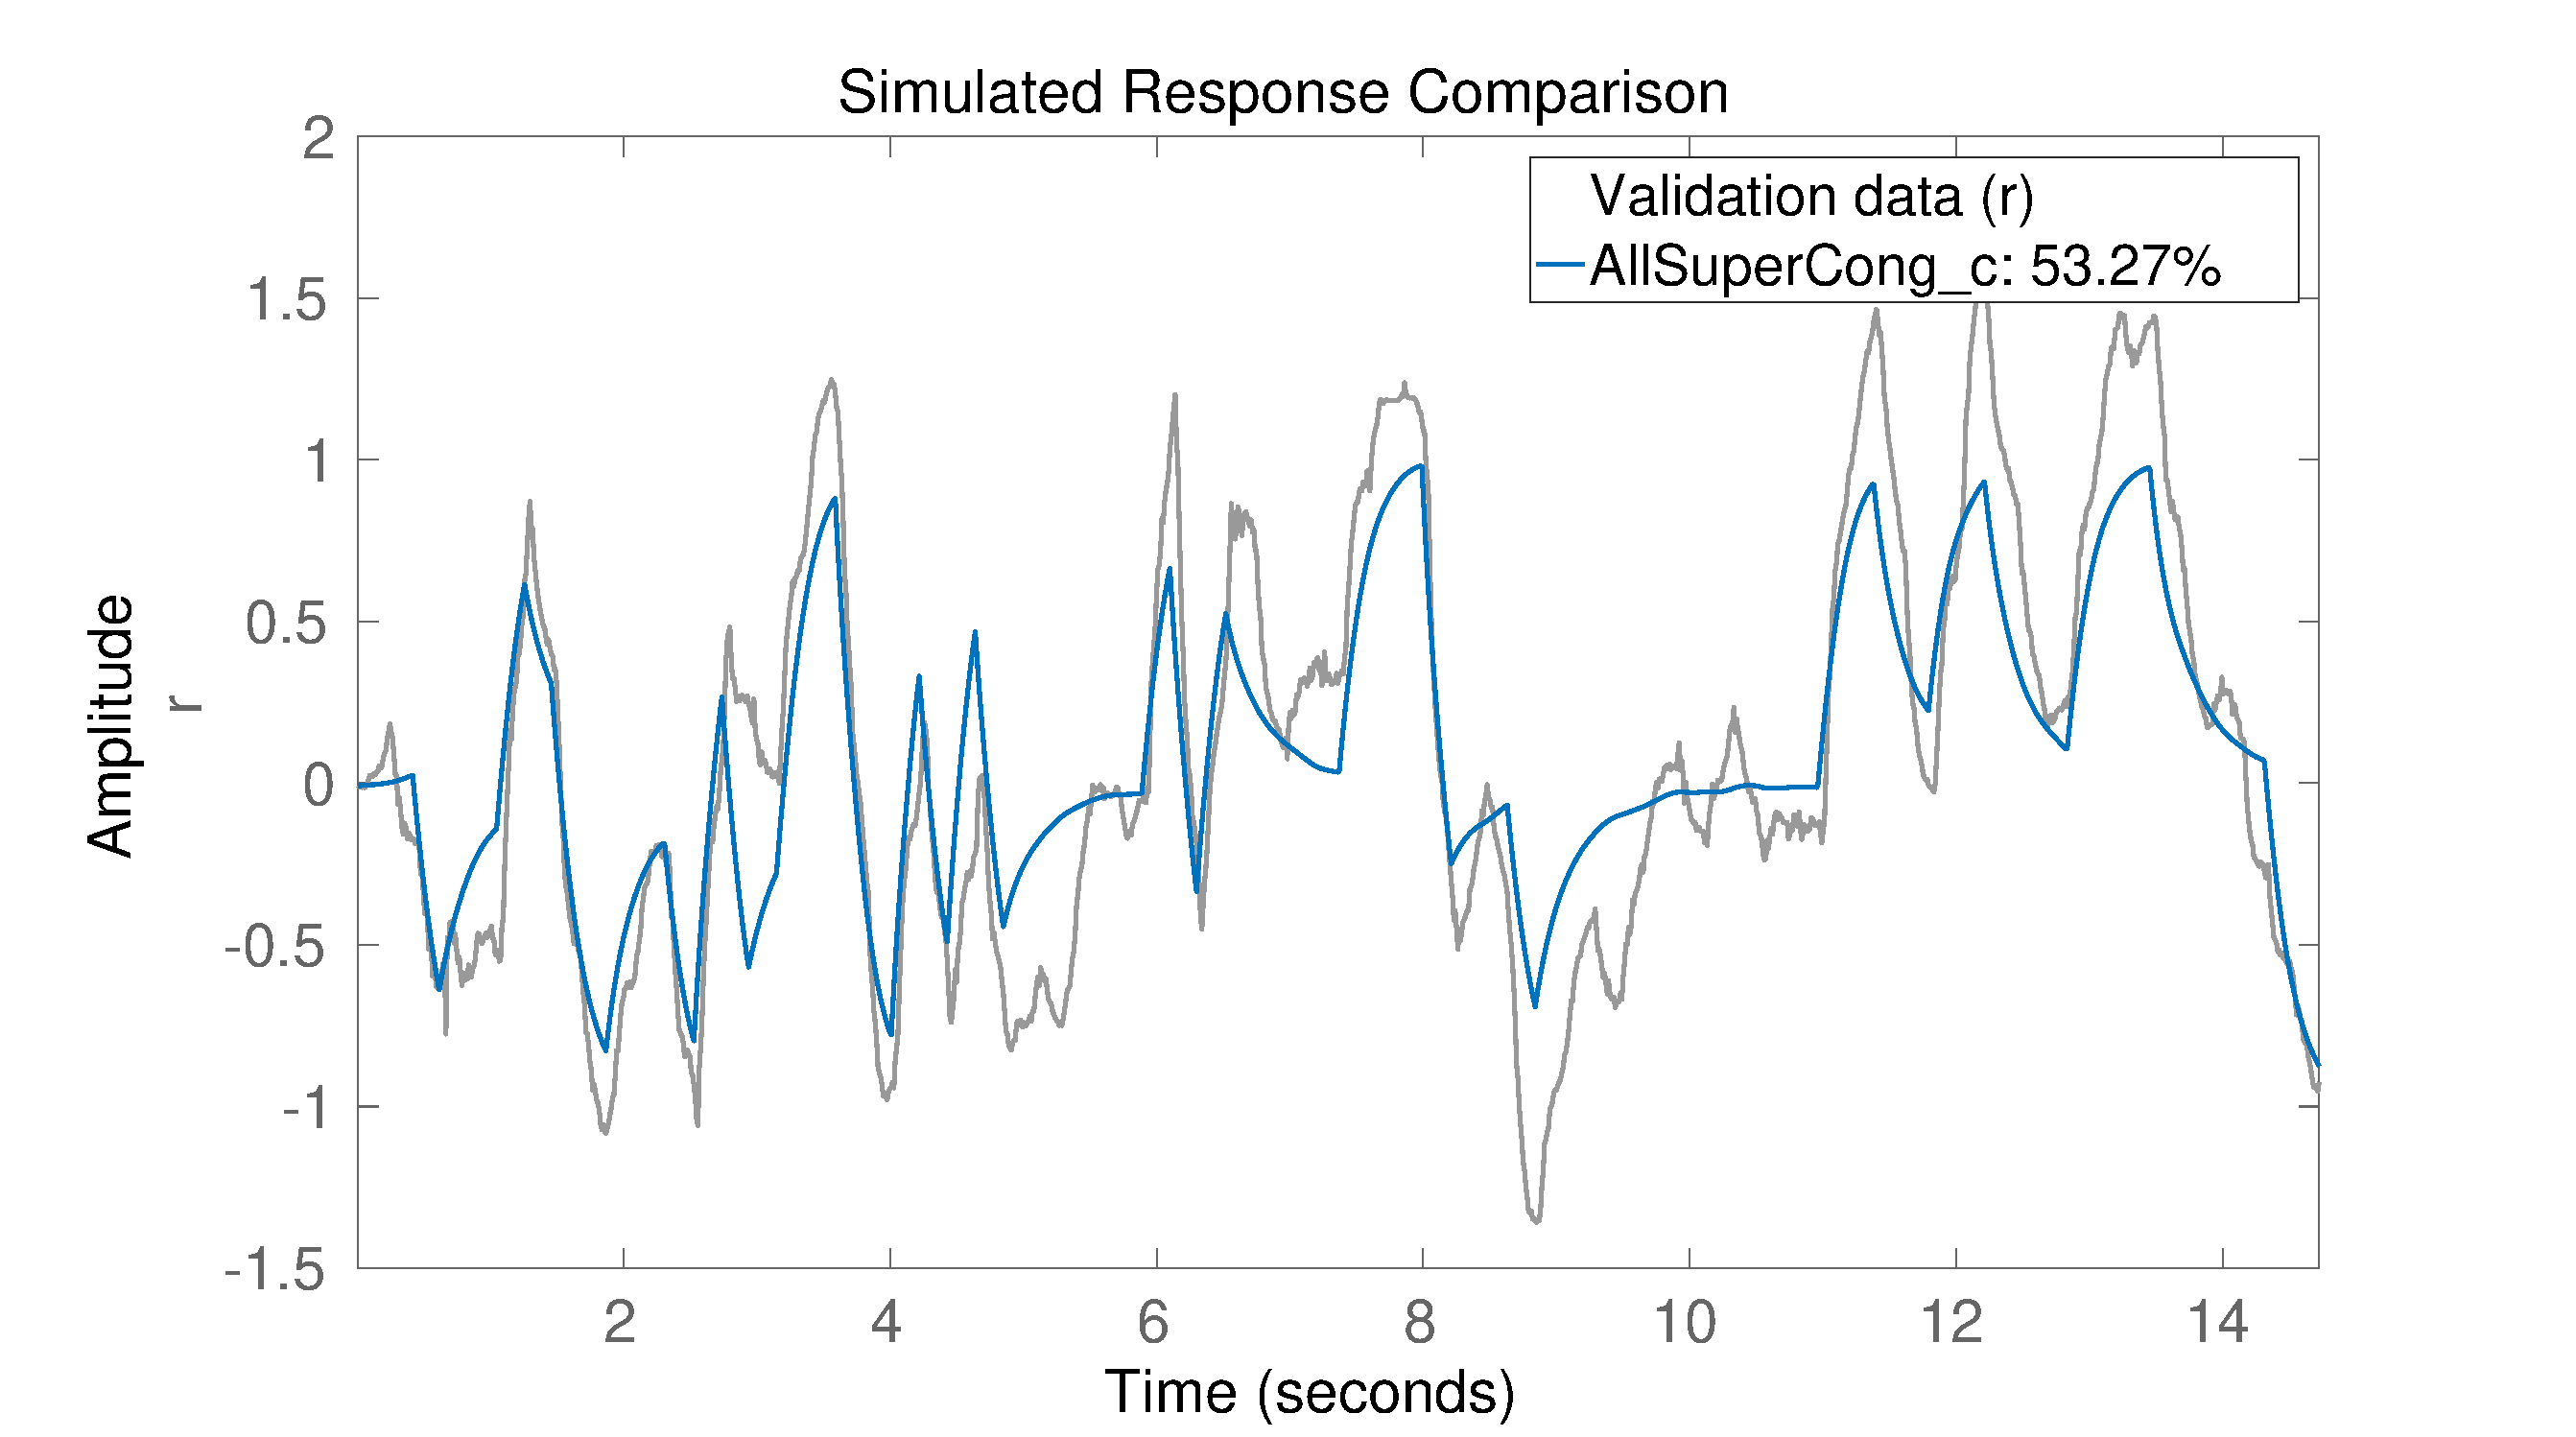
\includegraphics[width=0.4\textwidth]{angVelComparerlz6}}
    \qquad
  \subfloat[][\label{fig:linAccComparexlz6}Linear acceleration in the \abbrROV's x-axis.]{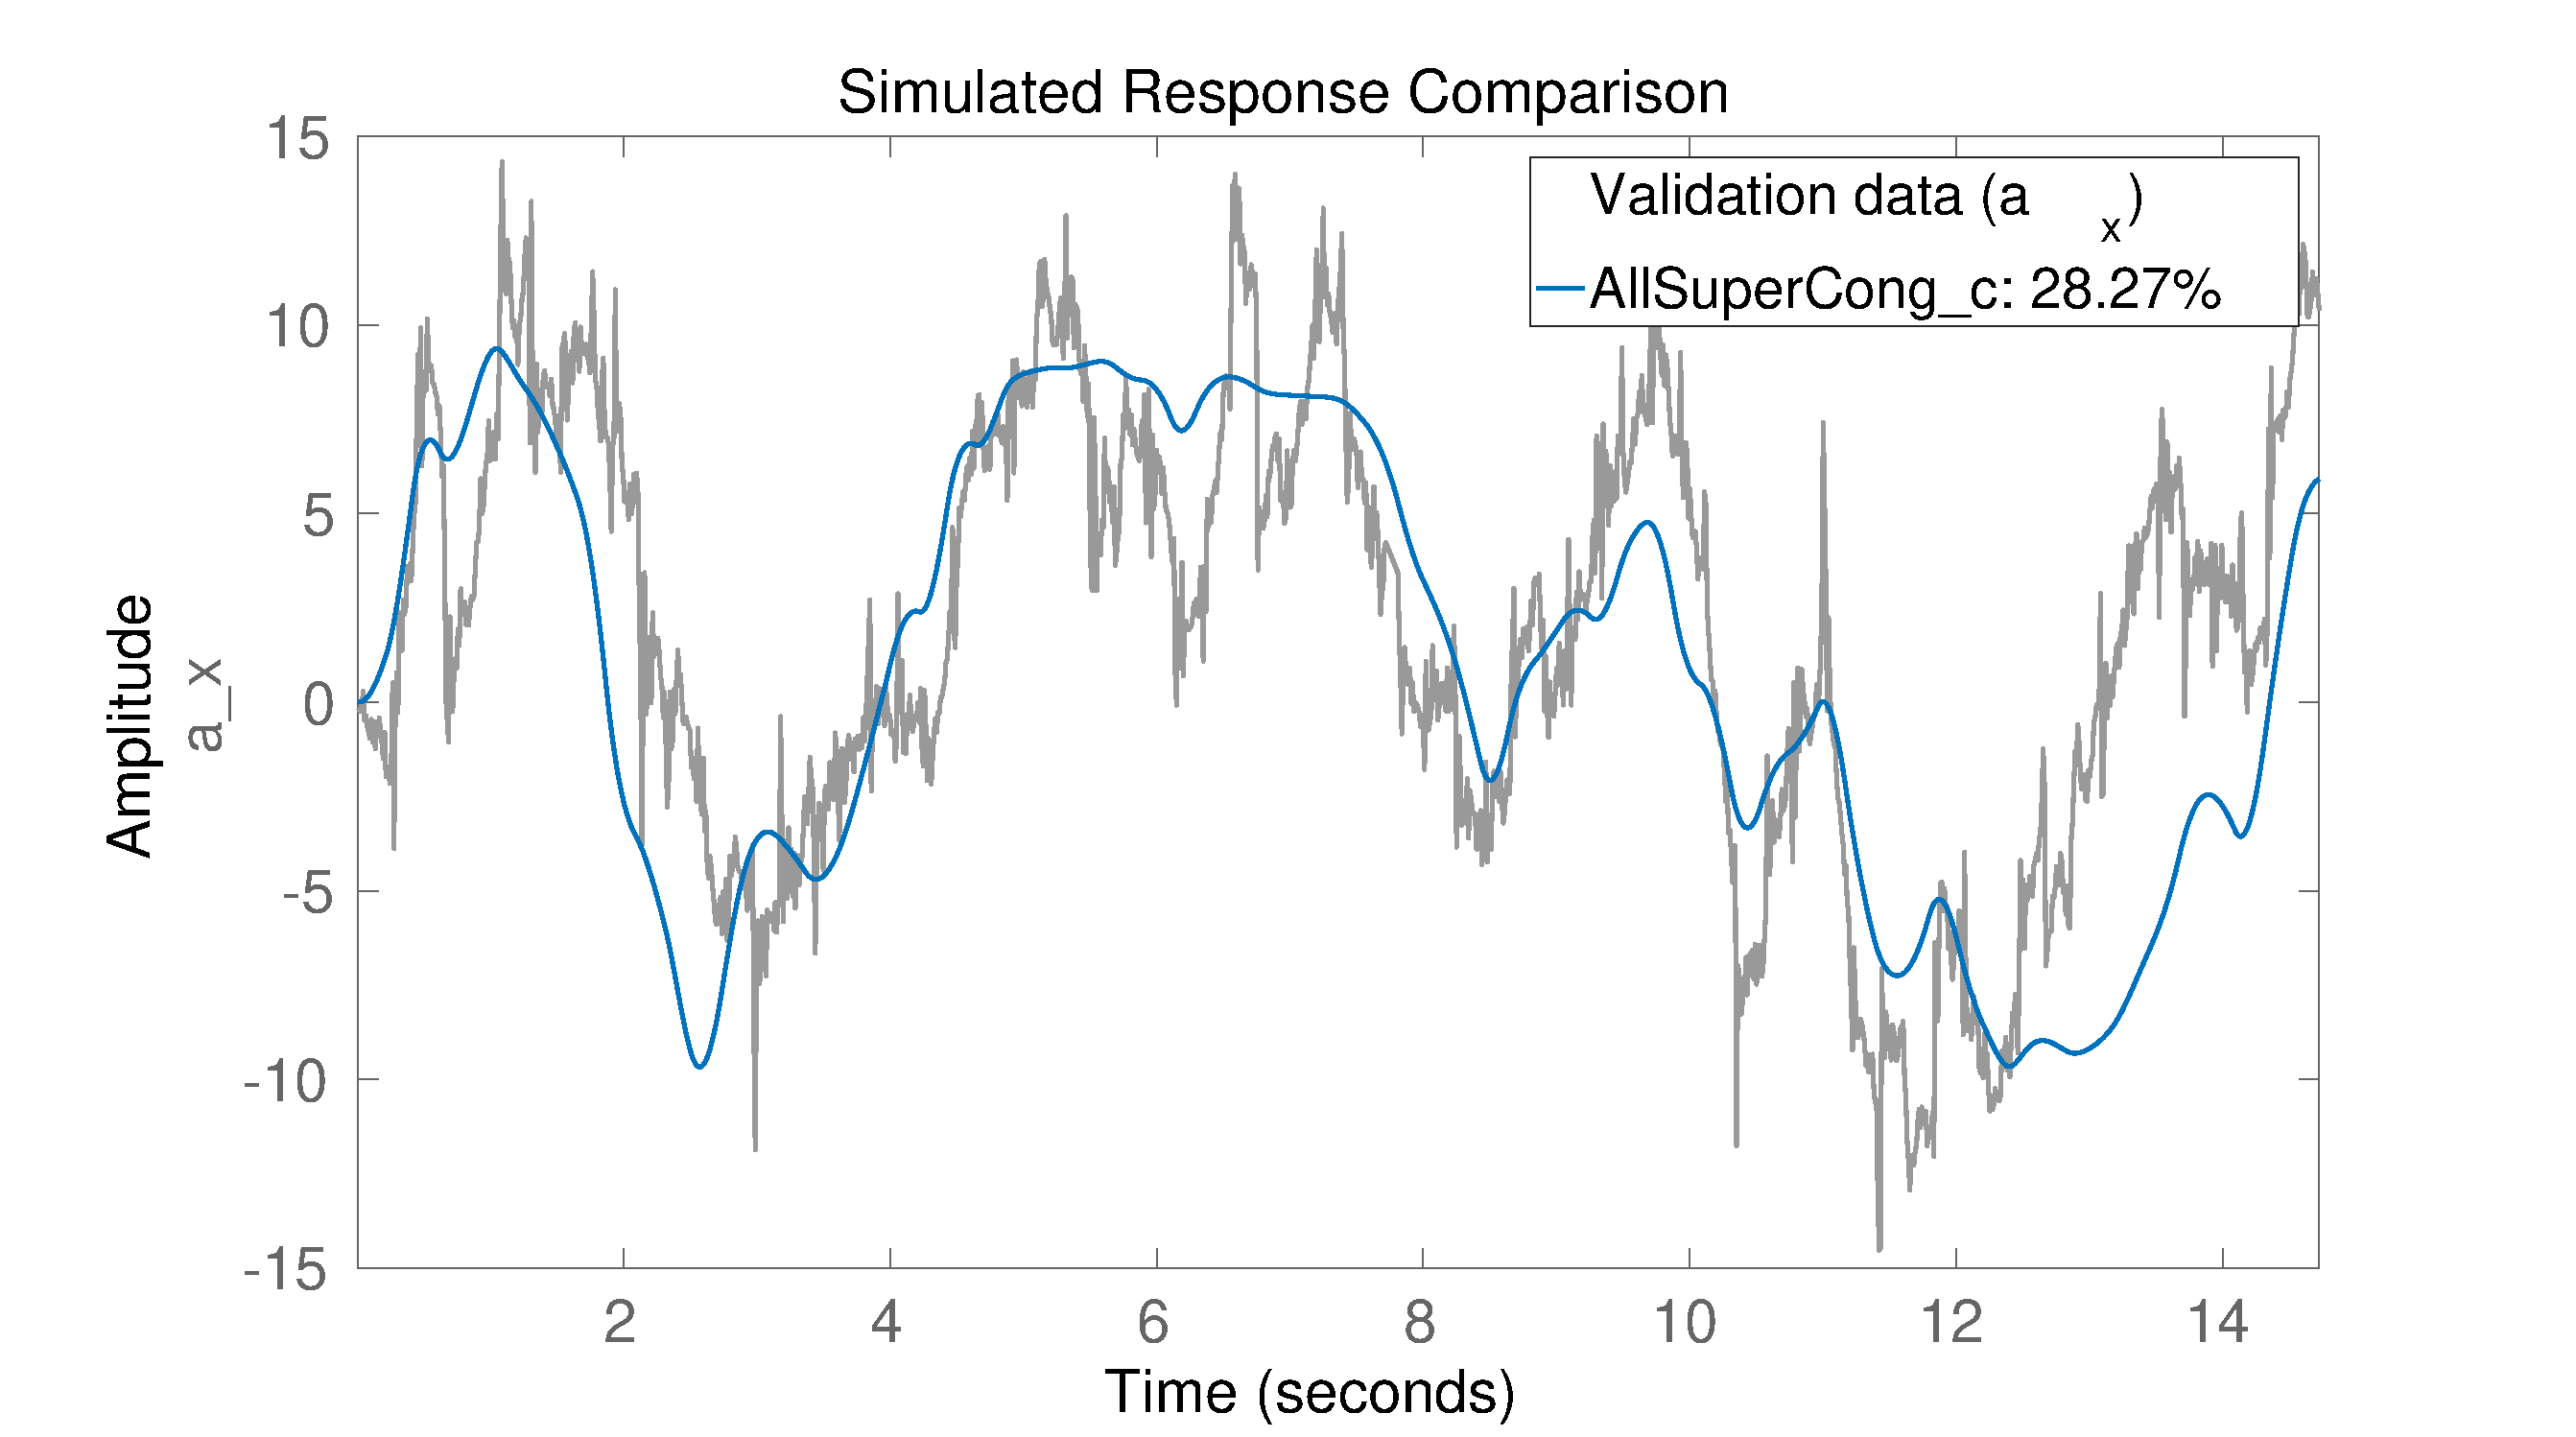
\includegraphics[width=0.4\textwidth]{linAccComparexlz6}}
    \qquad
  \subfloat[][\label{fig:linAccCompareylz6}Linear acceleration in the \abbrROV's y-axis.]{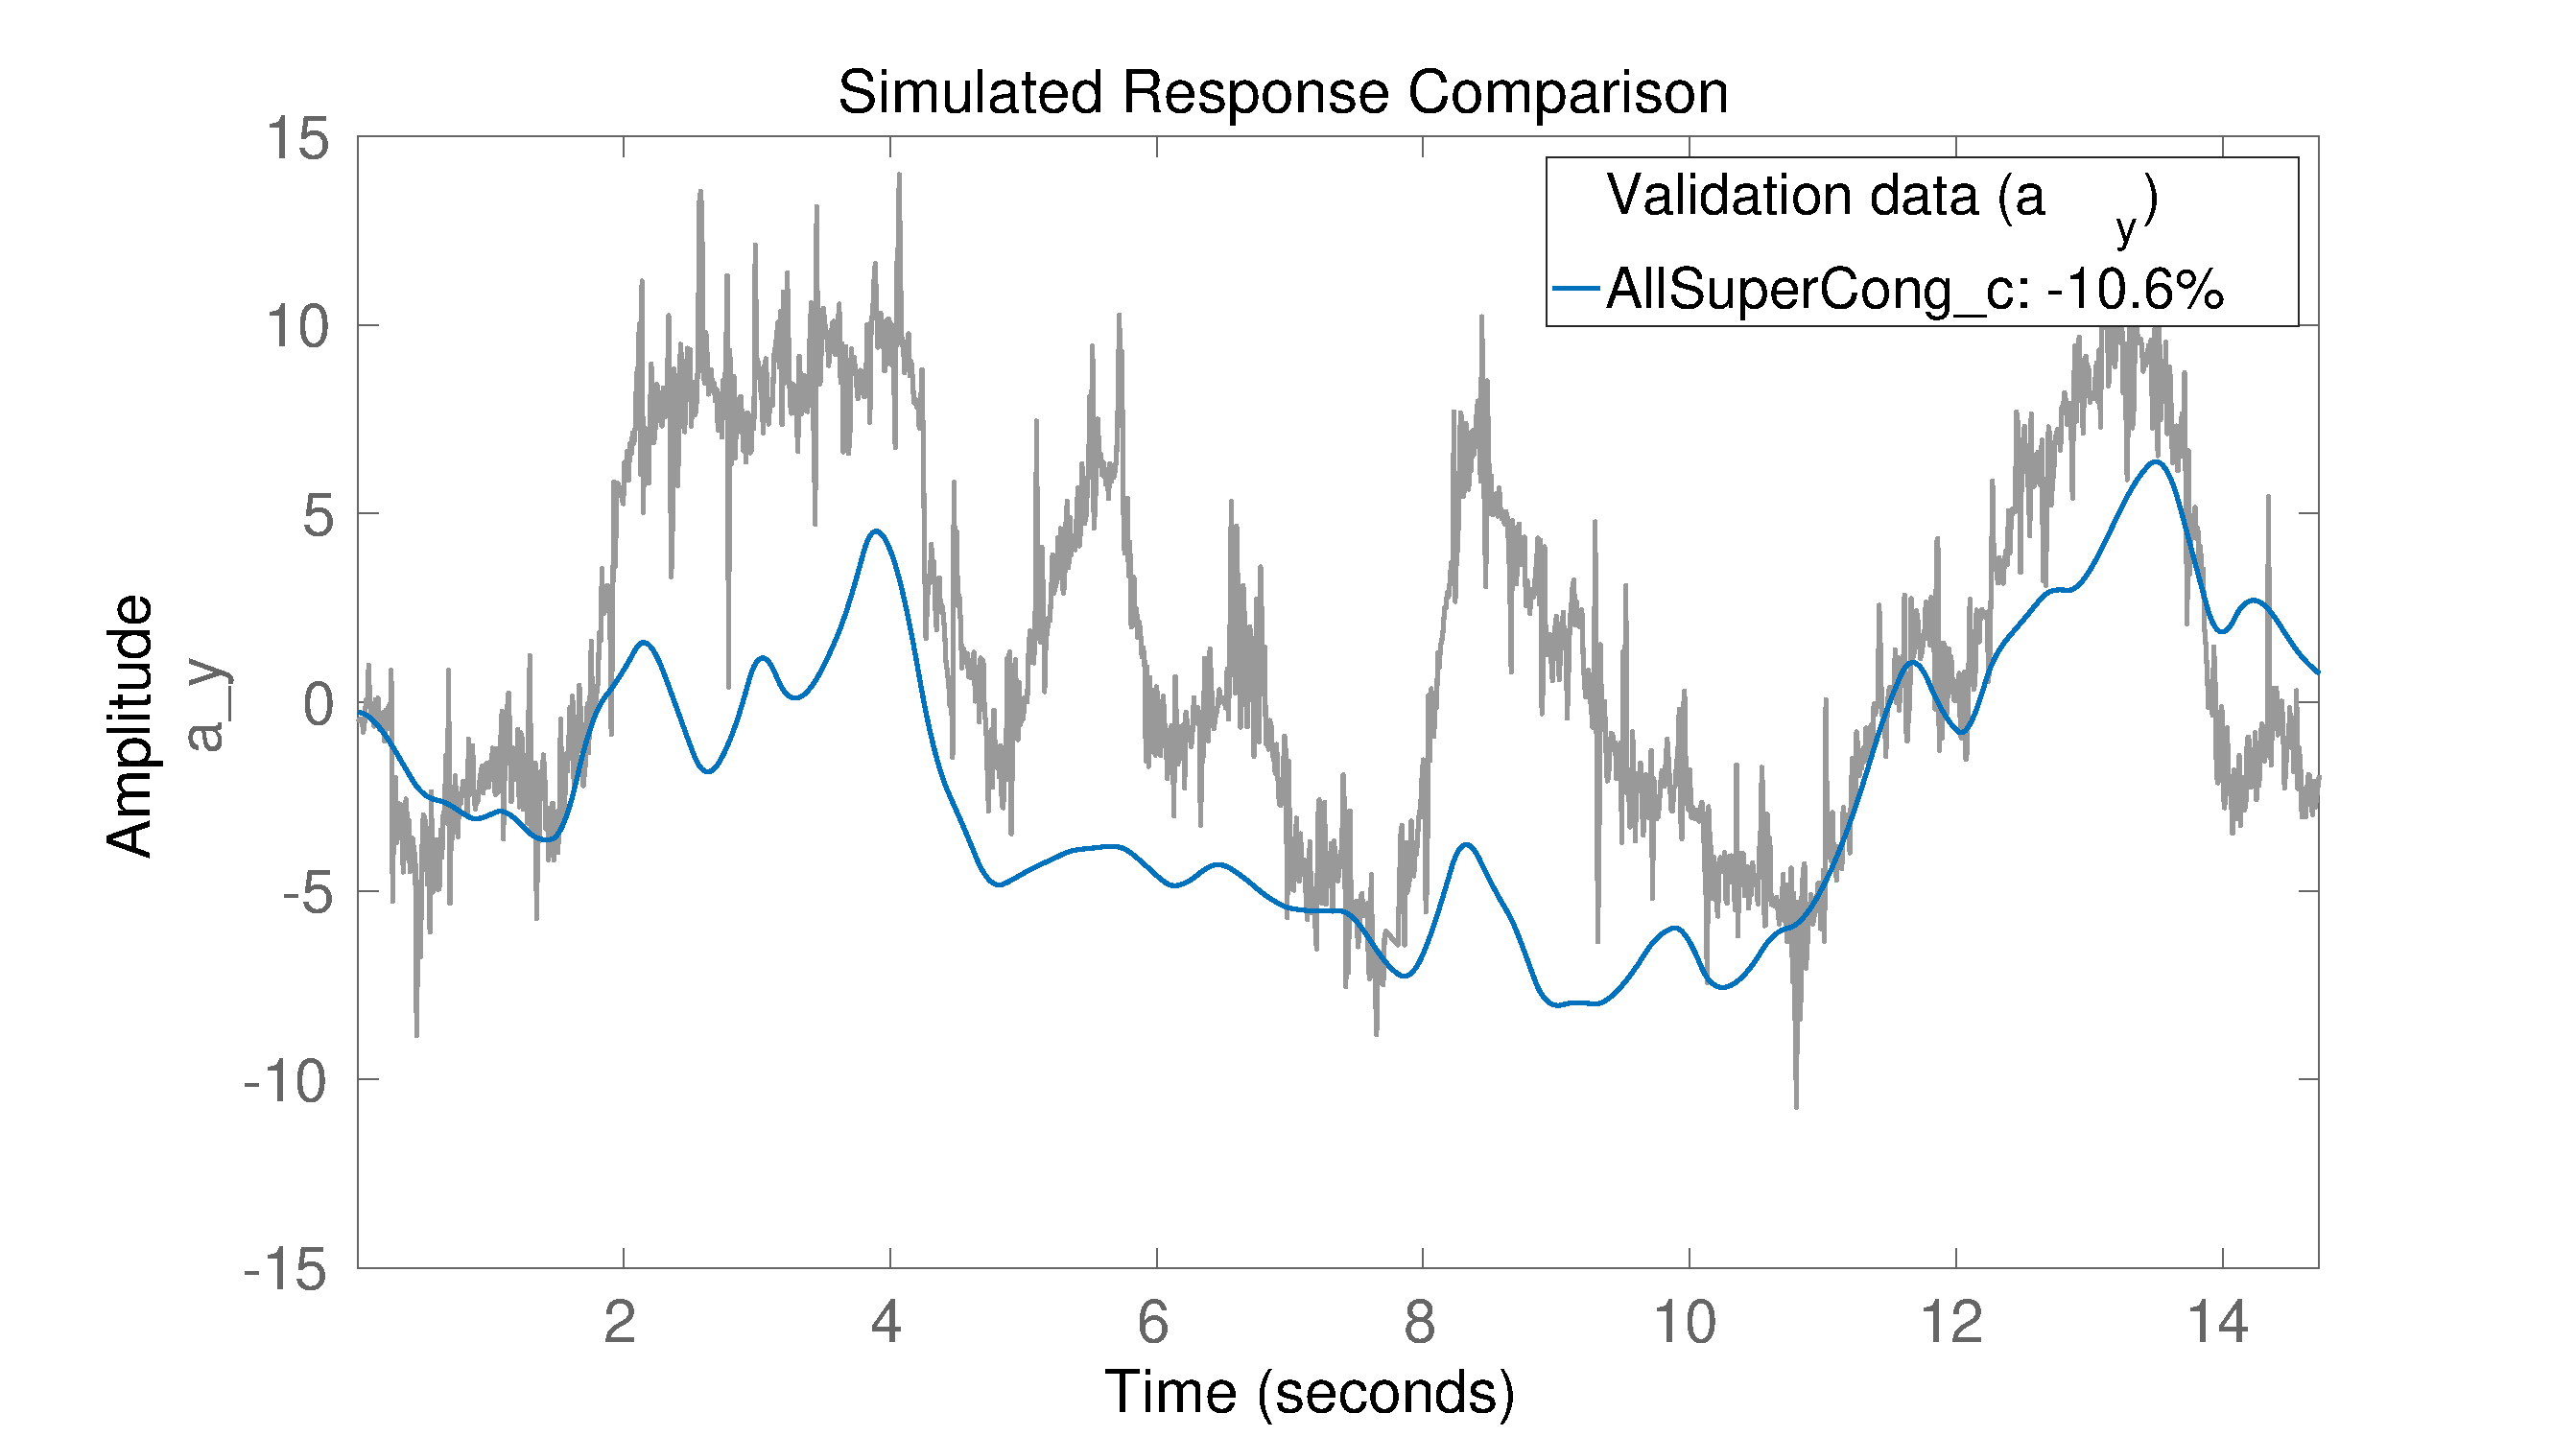
\includegraphics[width=0.4\textwidth]{linAccCompareylz6}}
    \qquad
  \subfloat[][\label{fig:linAccComparezlz6}Linear acceleration in the \abbrROV's z-axis.]{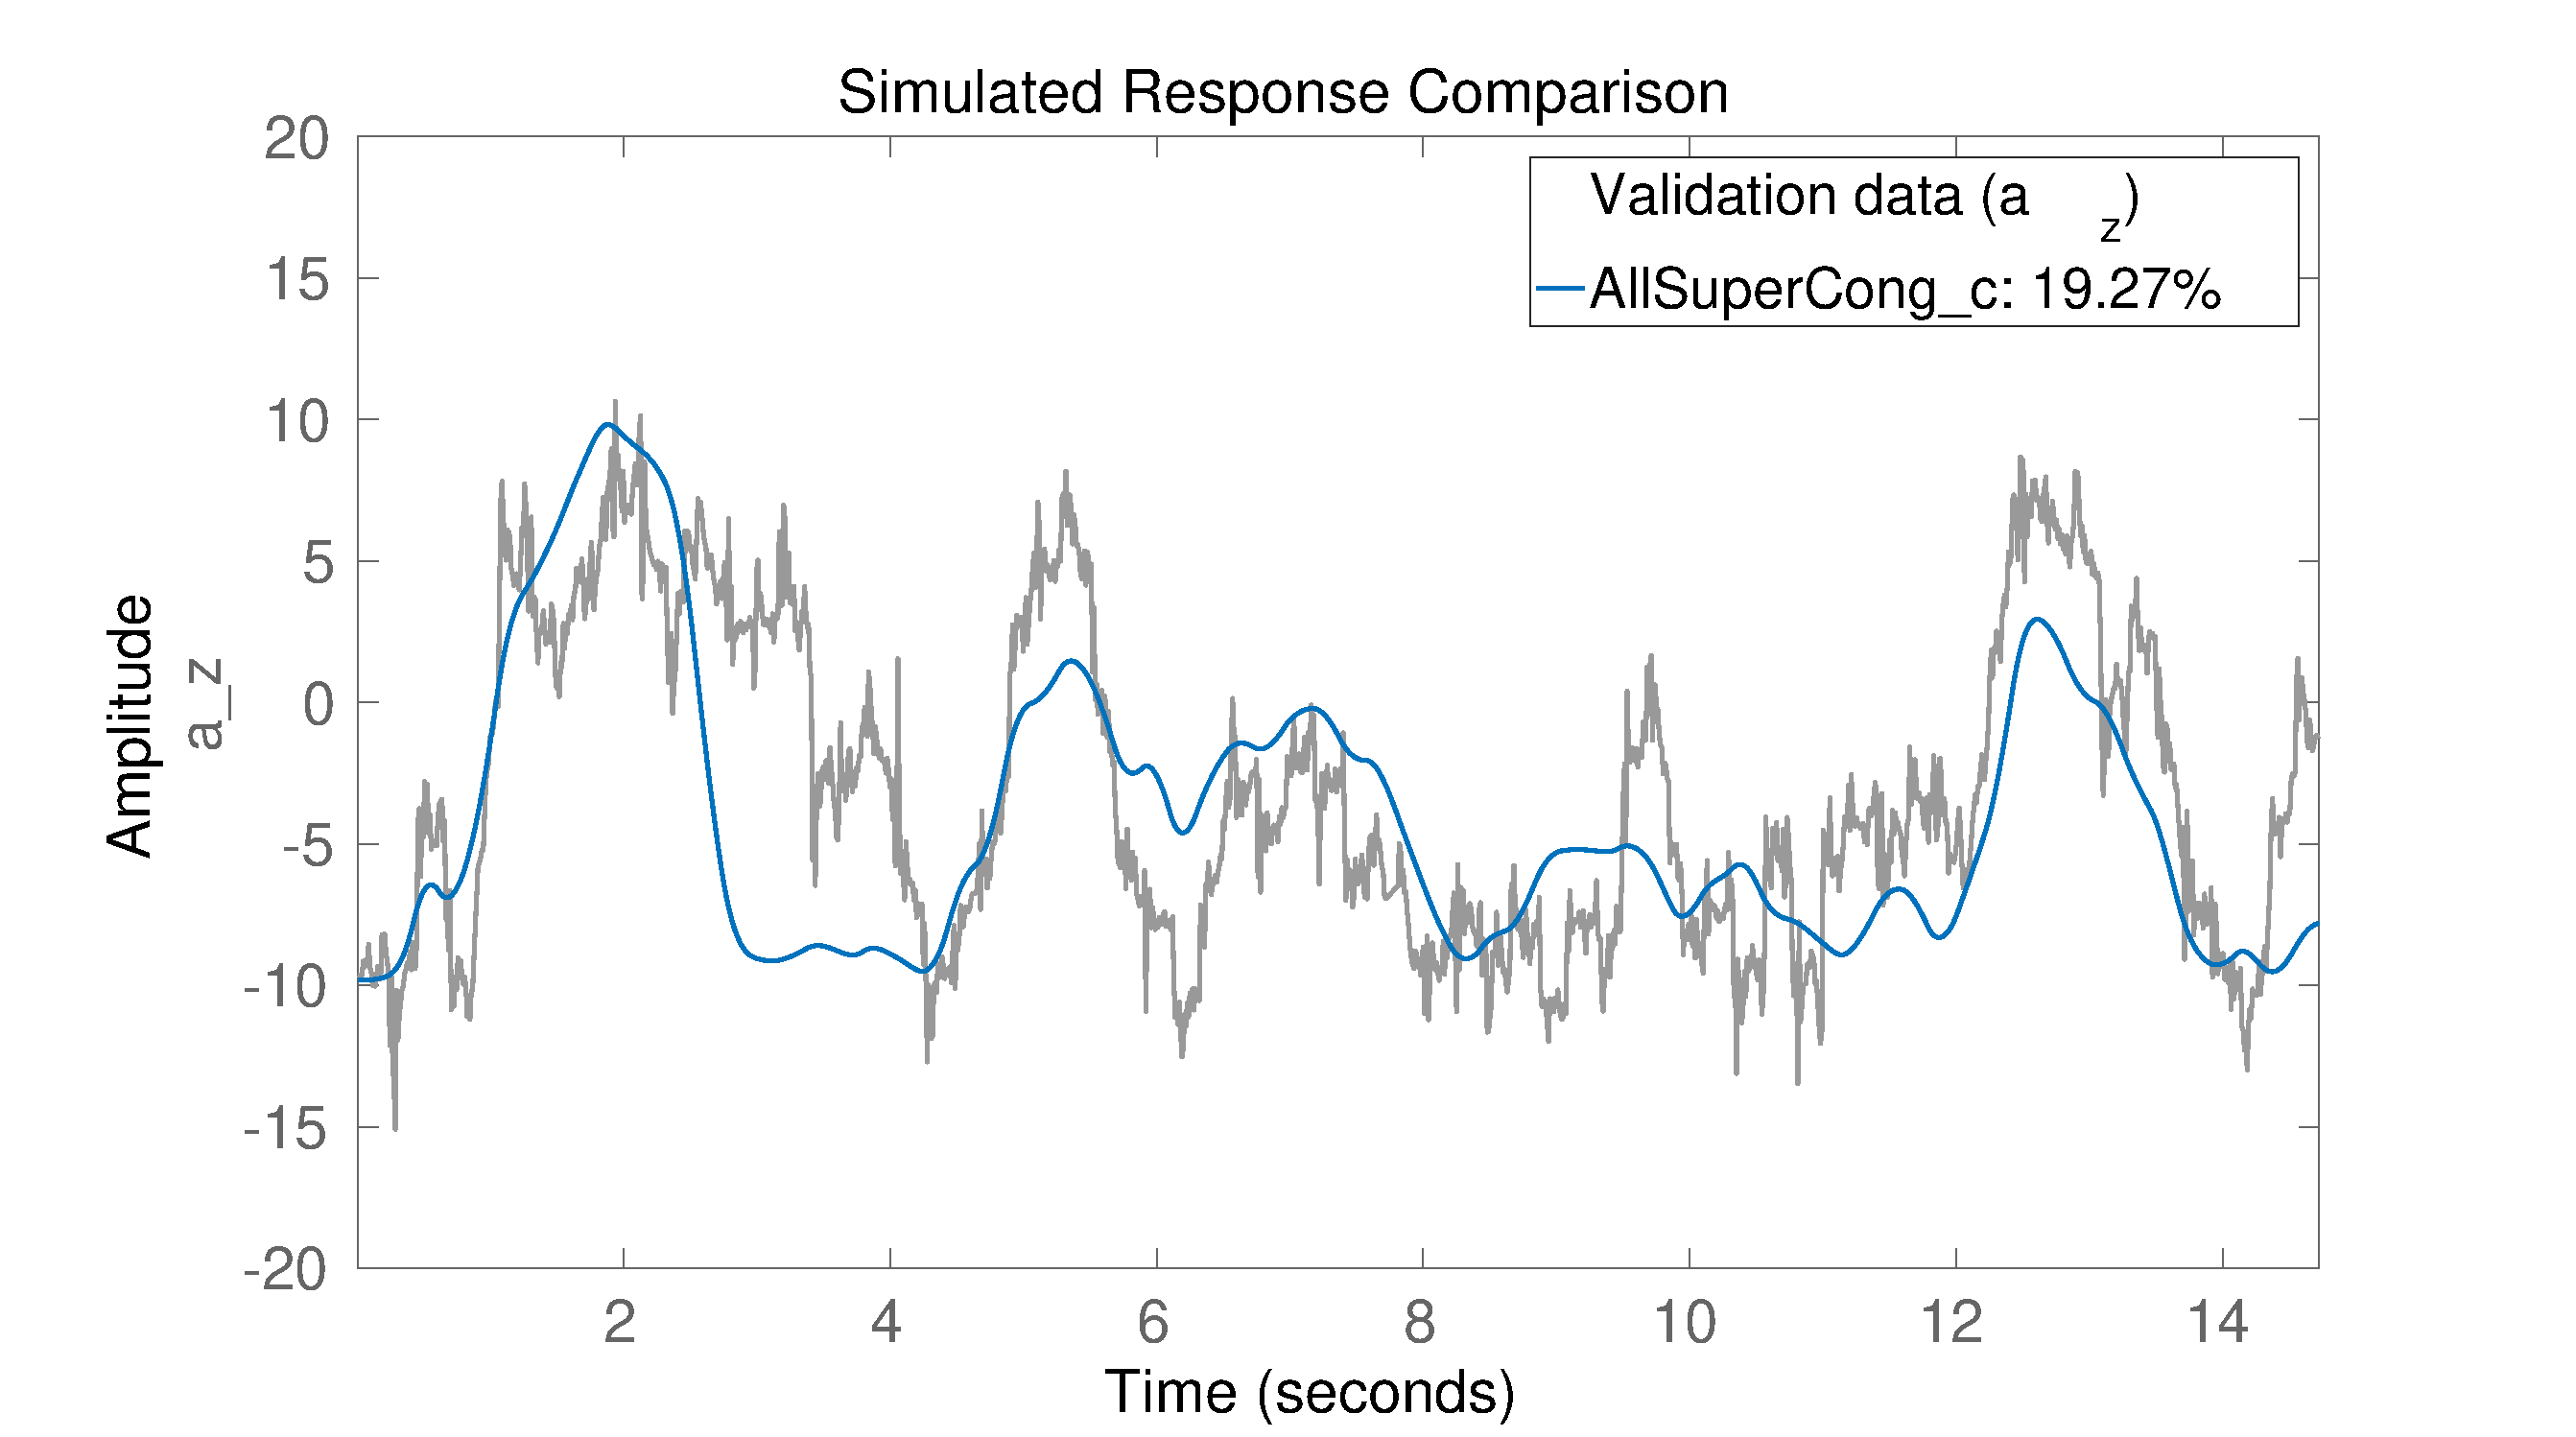
\includegraphics[width=0.4\textwidth]{linAccComparezlz6}}
  \caption{\label{fig:angVelComparelz6}%
    Comparison of validation data (grey) against the simulated response from the model(blue). The fit for the model in each state is stated in each plot. The estimation used angular velocities and linear accelerations as outputs. The model describes $q$ an $r$ well which can be seen in the high fit. The model do not describe the linear accelerations and $p$ well, this can be seen in the low fit.}
\end{figure}

\begin{table}[hbp]
  \centering
  \caption{\label{tab:ResultEstimAngular}%
    The estimated parameters from the prediction-error method using estimated angles as inputs and angular velocities as outputs (left) and the estimated parameters from the prediction-error method using angular velocities and linear acceleration as outputs (right).}
  \begin{tabular}{l p{0.18\linewidth} p{0.18\linewidth} p{0.18\linewidth}}
    \toprule%
    \textbf{Notation}  & \textbf{Starting Value} & \textbf{Estimated Value} & \textbf{Estimated Value}\\
    \otoprule%   
    % Parameters that will be estimated
	$z_B$               & -0.01 	\meter 						& -0.0178 \meter 						& -0.0294  	\meter\\
    $\Kp$               & -1   	\kilogram\usk\meter\squared 	& -1.3275  	\kilogram\usk\meter\squared	& -2.5940 	\kilogram\usk\meter\squared\\
    $\Kpabsp$           & -1  	\kilogram\usk\meter\squared	& 	0  		\kilogram\usk\meter\squared	& -0.3092  	\kilogram\usk\meter\squared\\
    $\Mq$               & -1  	\kilogram\usk\meter\squared	& -1.1925	\kilogram\usk\meter\squared	& -2.0425  	\kilogram\usk\meter\squared\\
    $\Mqabsq$           & -1  	\kilogram\usk\meter\squared	& -0.1094  \kilogram\usk\meter\squared	& -0.0071  	\kilogram\usk\meter\squared\\
    $\Nr$               & -1  	\kilogram\usk\meter\squared	&  -2.7838 	\kilogram\usk\meter\squared	& -2.9364	\kilogram\usk\meter\squared\\
    $\Nrabsr$           & -1  	\kilogram\usk\meter\squared	& -0.6751	\kilogram\usk\meter\squared	& -2.1843 	\kilogram\usk\meter\squared\\
    $A_p$               & 1.5 	\kilogram\usk\meter\squared	& 0.3255  	\kilogram\usk\meter\squared	& 0.7186 	\kilogram\usk\meter\squared\\
    $B_q$               & 1.5 	\kilogram\usk\meter\squared	& 0.3753 	\kilogram\usk\meter\squared	& 0.6112		\kilogram\usk\meter\squared\\
    $C_r$               & 1.5 	\kilogram\usk\meter\squared	& 0.9546 	\kilogram\usk\meter\squared	&  1.0981	\kilogram\usk\meter\squared\\
    \bottomrule%
  \end{tabular}
\end{table}   
%%%%%%%%%%%%%%%%%%%%%%%%%%%%%%%%%
\section{Extended Kalman Filter Estimation}\label{sec:KalmanEstimation}\index{EKF@\abbrEKF!abbreviation}
To circumvent the issues with estimating the initial state during the prediction-error method, a \abbrEKF was used to estimated the parameters. An \abbrEKF can  be used to estimate parameters by extending the state vector of the \abbrEKF with the parameters that need to be estimated \citep{Roger}.
\begin{equation}
\bar{\boldsymbol{x}} = \begin{bmatrix}
\boldsymbol{x}_k\\
\boldsymbol{\theta}_k
\end{bmatrix}
\end{equation}
The added parameters were modelled using constant position, which gave the following augmented state-space form 
\begin{equation}
\bar{\boldsymbol{x}}_{k+1}(\boldsymbol{\theta}) =\begin{bmatrix}
\boldsymbol{f}(\boldsymbol{x}_k(\boldsymbol{\theta}),\boldsymbol{u}_k,\boldsymbol{\theta})\\
\boldsymbol{\theta}_k
\end{bmatrix} 
+\boldsymbol{v}
\end{equation}
\begin{equation}
\boldsymbol{y}_k=\boldsymbol{h}(\bar{\boldsymbol{x}}_k(\boldsymbol{\theta}),\boldsymbol{u}_k)
\end{equation}
Since the \abbrEKF tries to minimise state variance it will also try to estimate the parameters $\boldsymbol{\theta}$ if they are included in the state vector \citep{Roger}.

%\subsection{Implementation}\label{sec:KalmanEstimatorImpl}
%The reparametrised model \eqref{eq:quatModel} was used to model $\etaVector$ and $\nuVector$. Measurement equations were taken from \Chapterref{cha:sensor_fusion}. Each model parameter was modelled as a state using a constant position motion model and the motion model was discretised using the Euler forward discretisation method. The complete discrete model is
%\begin{equation}
%\label{eq:motionModelKalman}
%\begin{pmatrix}
%\etaVector_{k+1}\\ 
%\nuVector_{k+1}\\
%\boldsymbol{b}_{k+1}\\
%\boldsymbol{\theta}_{k+1}
%\end{pmatrix} = 
%\begin{pmatrix}
%\etaVector_k + T_s \boldsymbol{T}(\etaVector_k)\nuVector_k\\
%\nuVector_k + T_s f(\etaVector_k,\nuVector_k,\boldsymbol{\theta}_k)\\
%\boldsymbol{b}_k\\
%\boldsymbol{\theta}_k
%\end{pmatrix}
%+ \begin{pmatrix}
%\boldsymbol{v}_{\etaVector}\\
%\boldsymbol{v}_{\nuVector}\\
%\boldsymbol{v}_{\boldsymbol{b}}\\
%\boldsymbol{v}_{\boldsymbol{\theta}}
%\end{pmatrix}
%\end{equation}
%Here, $\boldsymbol{\theta}$ is a vector containing the parameters that were estimated. The vector-valued function $\boldsymbol{f}(\etaVector,\nuVector,\boldsymbol{\theta})$ is \eqref{eq:quatModel}. The vector $\boldsymbol{b}$  contains the biases of the gyroscope. The vector $\boldsymbol{v}$ is the system noise and is assumed to enter each term directly, this resulted in a diagonal $\boldsymbol{Q}$-matrix when implementing the model in the \abbrEKF. The matrix $\boldsymbol{T}(\etaVector)$ is an angular velocity transformation matrix using the quaternion form of $\etaVector$ and is defined in \Chapterref{cha:modelling}. Measurement equations are taken from \sectionref{sec:Meas}.

To increase the performance of the filter a method for outlier detection and rejection was implemented. Since time updates were done batch wise it was decided to use a different form of outlier rejection and not to reimplement the method used in \sectionref{sec:Meas}. The outlier rejection method is based on the assumption that the normalised innovation \begin{equation} \label{eq:chi}
\boldsymbol{\epsilon}^T \boldsymbol{S}^{-1} \boldsymbol{\epsilon} \sim \chi_{n}^{2}
\end{equation}
where $n$ is the number of measurements. To check the validity of a single measurement, \eqref{eq:chi} gives that $\epsilon_i^{2}/S_{i,i} \sim \chi_{1}^{2}$ \citep{sensorfusion}. This is implemented in the \abbrEKF using \Algoref{alg:outlier}.
\begin{algorithm}[h]
\caption{The outlier rejection algorithm used during the measurement update step of the parameter estimation \abbrEKF.}\label{alg:outlier}
\textbf{1.} Calculate $\boldsymbol{S}=h_{\boldsymbol{x}} \boldsymbol{P} h_{\boldsymbol{x}}^T + \boldsymbol{R}$ and the innovation $\epsilon$.
\\
\textbf{2.} For each row $i$ in $\boldsymbol{\epsilon}$ do the comparison
\begin{equation}
\epsilon_{i}^{2} > \sigma_i S_{i,i}
\end{equation}
If the expression holds true, remove the $i$:th row from $\boldsymbol{\epsilon}$ and the $i$:th row and column from $\boldsymbol{S}$ and $h_{\boldsymbol{x}}$.\\
\textbf{3.} Proceed with the Kalman algorithm using the cropped $h_{\boldsymbol{x}}$, $\boldsymbol{S}$ and $\boldsymbol{\epsilon}$.

Here, $\boldsymbol{\sigma}$ is a $n\times1$ dimensional design variable and $n$ is the number of measurements that are used in the \abbrEKF. A higher value of $\sigma_i$ decreases the sensitivity of the outlier rejection for the $i$:th measurement.
\end{algorithm}

%The filter was run on each collected dataset. The final values of $\hat{\boldsymbol{\theta}}$ from a dataset were used as initial values for $\hat{\boldsymbol{\theta}}$ when the filter was applied on the next dataset. The same was done for the covariance matrix $\boldsymbol{P}$. The final covariance from an earlier run was set as the initial covariance when the filter was applied on subsequent dataset. At completion the parameters were entered in a simulator which was feed with the control signals from the corresponding dataset. The simulated  output was then compared with the original data.

\section{Estimation Using an Extended Kalman Filter}
The \abbrEKF estimation used the method described in \sectionref{sec:KalmanEstimation} with the model \eqref{eq:quatModel} and quaternions as attitude representation. The estimation was feed with process noise covariance matrix
\begin{equation*}
\boldsymbol{Q}=\text{diag}[\underbrace{\overbrace{100}^{\times4}}_{\etaVector}... \underbrace{\overbrace{1000}^{\times3}}_{\nuVector}...\underbrace{\overbrace{0.01}^{\times3}}_{\boldsymbol{b}}... \underbrace{\overbrace{0.01}^{\times10}... \overbrace{0.000001}^{\times5}}_{\boldsymbol{\theta}}]\text{ ,}
\end{equation*}
measurement noise covariance matrix
\begin{equation*}
\boldsymbol{R} = \text{diag}[\underbrace{\overbrace{0.01}^{\times3}}_{\text{Gyro}}... \underbrace{\overbrace{0.1}^{\times3}}_{\text{Acc}}... \underbrace{\overbrace{100}^{\times3}}_{\text{mag}}]
\end{equation*}
The extremely low values of the last five elements in $\boldsymbol{Q}$ were chosen to fixate the measured moment arms of the thrusters. Four data sets were feed in to the estimator and a fifth was used as validation data. All data sets were of excitations in $p$, $q$ and $r$ simultaneously. Parameter values from the estimation can be viewed together with the starting state in \tableref{tab:ResultKalmanFixedMomentArms}. \todo[inline]{kolla med jonas om laga varden}
\begin{table}[hbp]
  \centering
  \caption{\label{tab:ResultKalmanFixedMomentArms}%
    The estimated parameters from the Kalman estimator method. Moment arms are fixed to measured values.}
  \begin{tabular}{l l p{0.25\linewidth}}
    \toprule%
    \textbf{Notation}  & \textbf{Starting Value} & \textbf{Estimated Value} \\
    \otoprule%   
    % Parameters that will be estimated
    $\etaVector$			&$[1\ 0\ 0\ 0]^T$					&\\
    $\nuVector$			&$[0\ 0\ 0]^T$						&\\
    $\boldsymbol{b}$		&$[0\ 0\ 0]^T$						&\\
	$z_B$               & -0.05 	\meter 						& -0.0606  	\meter\\
    $\Kp$               & -1   	\kilogram\usk\meter\squared 	& -0.8745 		\kilogram\usk\meter\squared\\
    $\Kpabsp$           & -1  	\kilogram\usk\meter\squared	& -0.6279  		\kilogram\usk\meter\squared\\
    $\Mq$               & -1  	\kilogram\usk\meter\squared	& -0.8529  		\kilogram\usk\meter\squared\\
    $\Mqabsq$           & -1  	\kilogram\usk\meter\squared	& -0.2505  	\kilogram\usk\meter\squared\\
    $\Nr$               & -1  	\kilogram\usk\meter\squared	& -1.0469		\kilogram\usk\meter\squared\\
    $\Nrabsr$           & -1  	\kilogram\usk\meter\squared	& -1.0405 		\kilogram\usk\meter\squared\\
    $A_p$               & 1 	\kilogram\usk\meter\squared	&  0.9728 		\kilogram\usk\meter\squared\\
    $B_q$               & 1 	\kilogram\usk\meter\squared	&  0.7266		\kilogram\usk\meter\squared\\
    $C_r$               & 1 	\kilogram\usk\meter\squared	&  1.2013		\kilogram\usk\meter\squared\\
    $\distance{x}{1}$  &0.19 \meter & 0.1900 \meter\\
    $\distance{y}{1}$  &0.11 \meter & 0.1106 \meter\\
    $\distance{x}{2}$  &0.19 \meter & 0.1900 \meter\\
    $\distance{y}{2}$  &0.11 \meter & 0.1106 \meter\\
    $\distance{y}{3}$  &0.11 \meter & 0.1099 \meter\\
    $\distance{x}{5}$  &0.17 \meter & 0.1704 \meter\\
    $\distance{y}{4}$  &0.11 \meter & 0.1099 \meter\\
    $\distance{z}{6}$  &0.11 \meter & 0.1091 \meter\\ 
    \bottomrule%
  \end{tabular}
\end{table}
The fit of the model using the estimated parameters can be viewed in \figureref{fig:ResultKalmanFixedMomentArms}. The high fit in $q$ and $r$ indicate that the model describes the data well. However, the model do not describe the validation data well in $q$.
% results kalman fixed moment arms
\begin{figure}[tbp]
  \centering
  \subfloat[][Comparison between a simulated model response and validation data in $p$.]{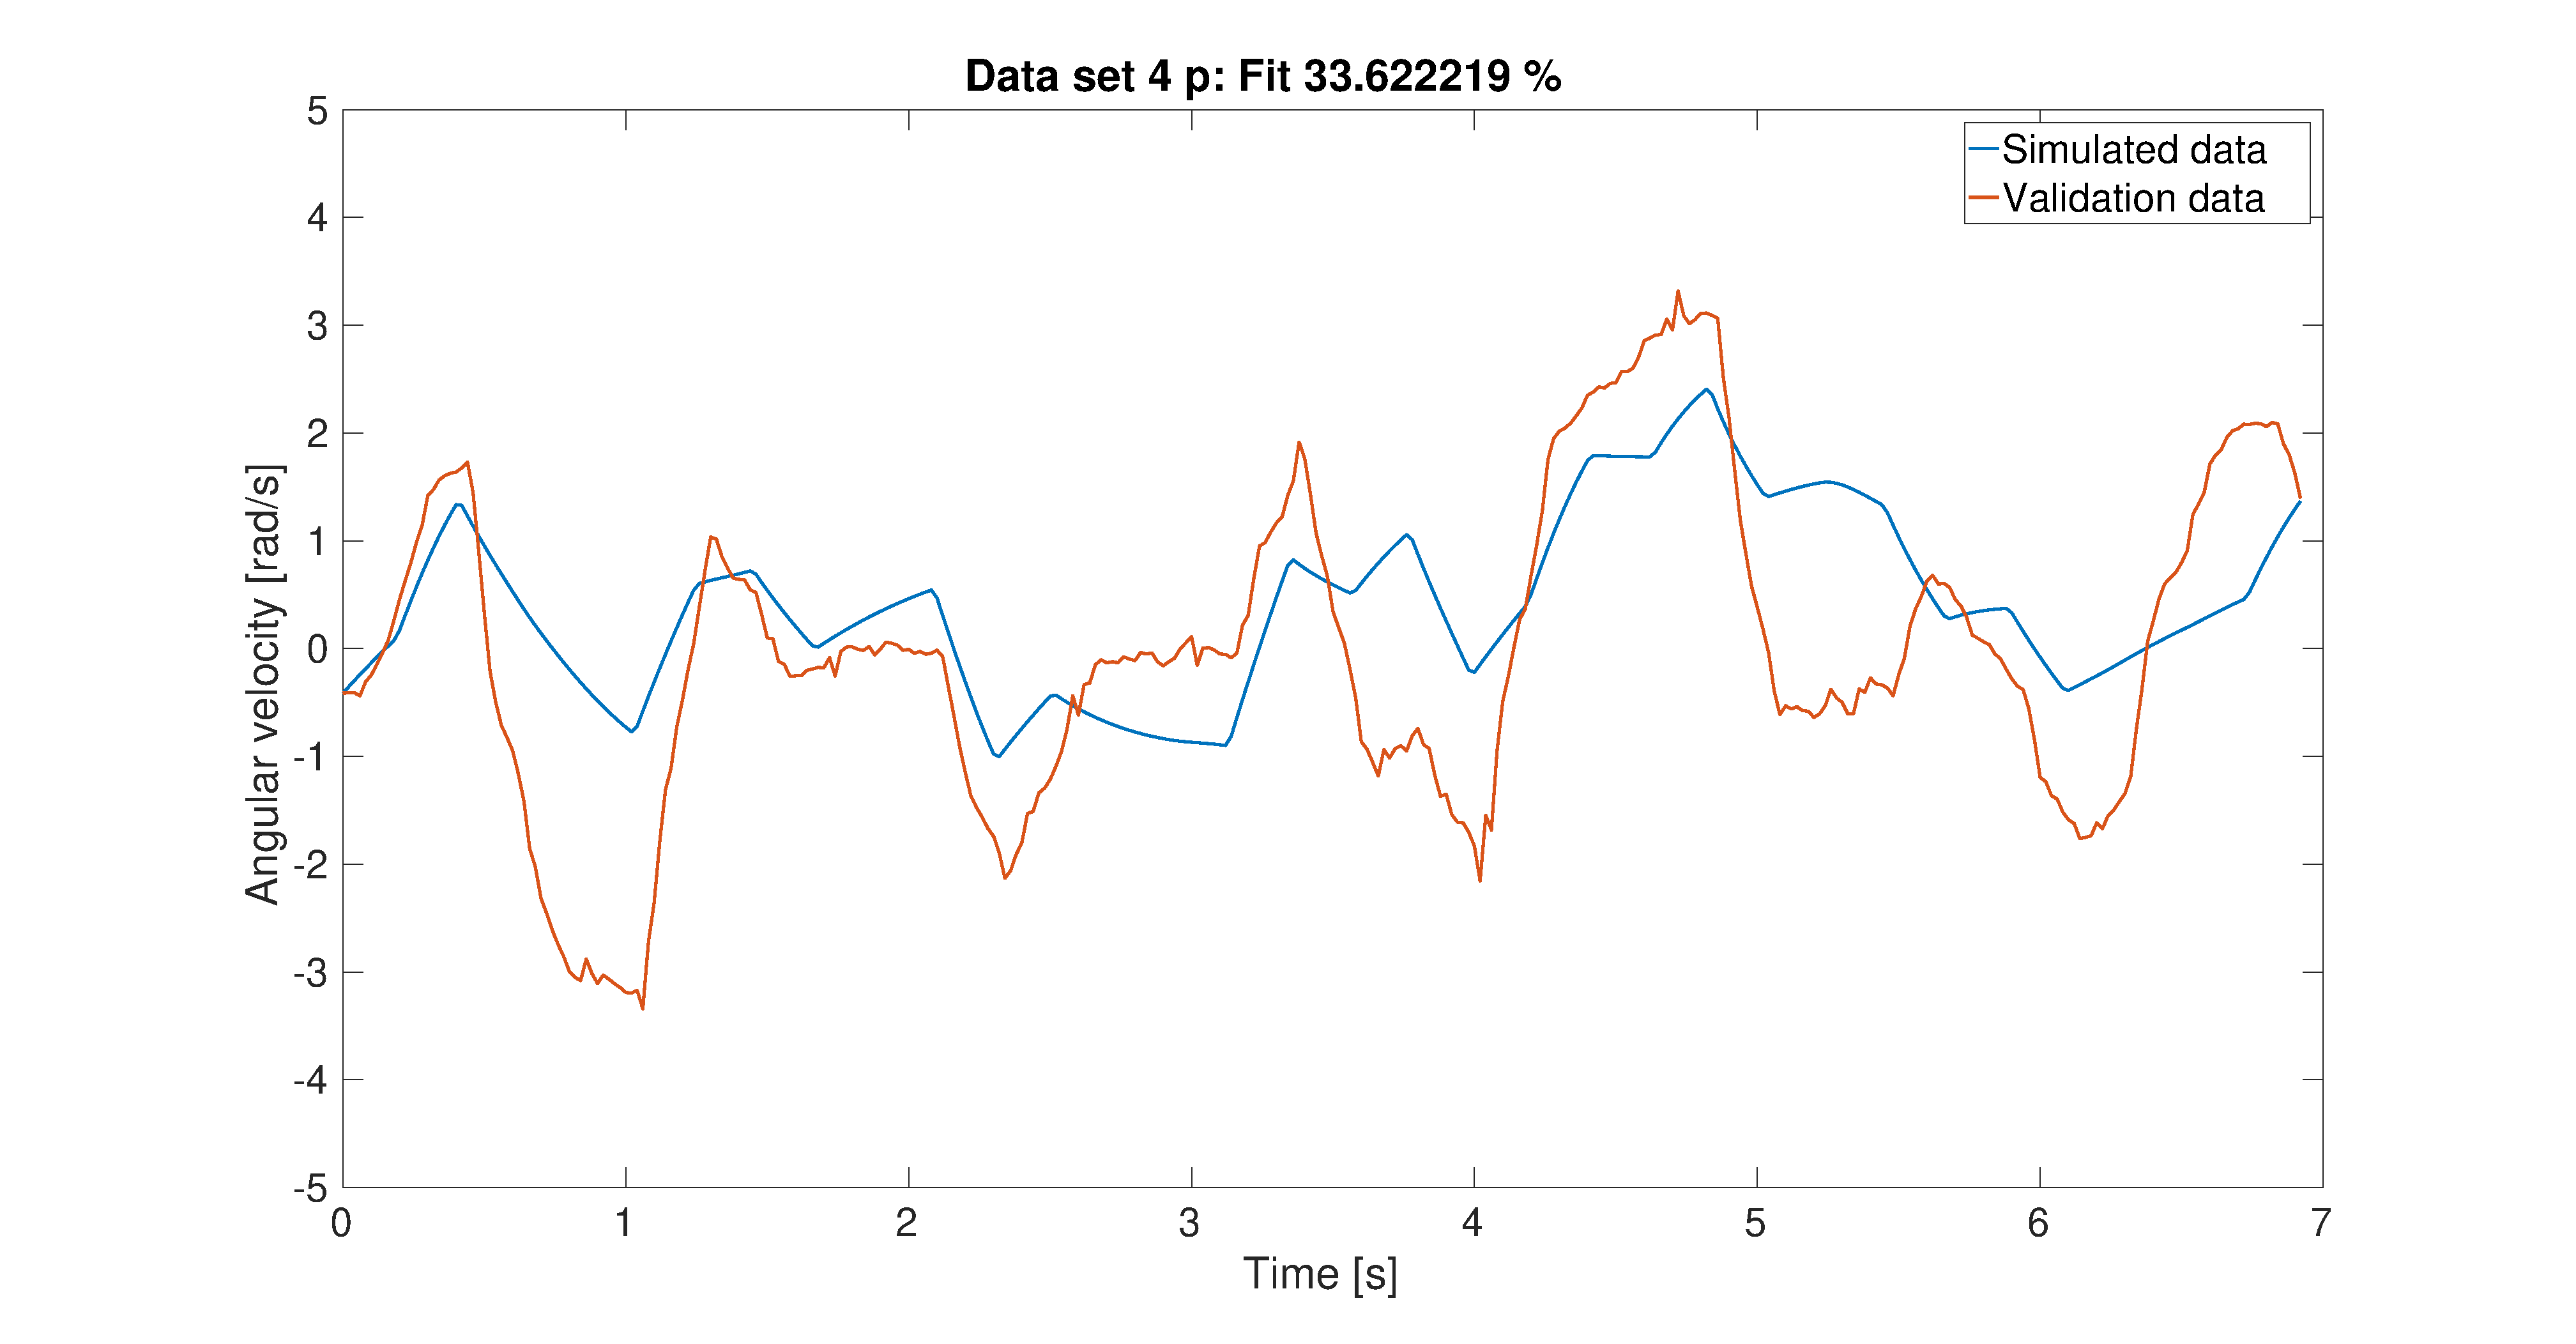
\includegraphics[width=0.7\textwidth]{ResultKalmanFixedMomentP}}
  \qquad
  \subfloat[][Comparison between a simulated model response and validation data in $q$.]{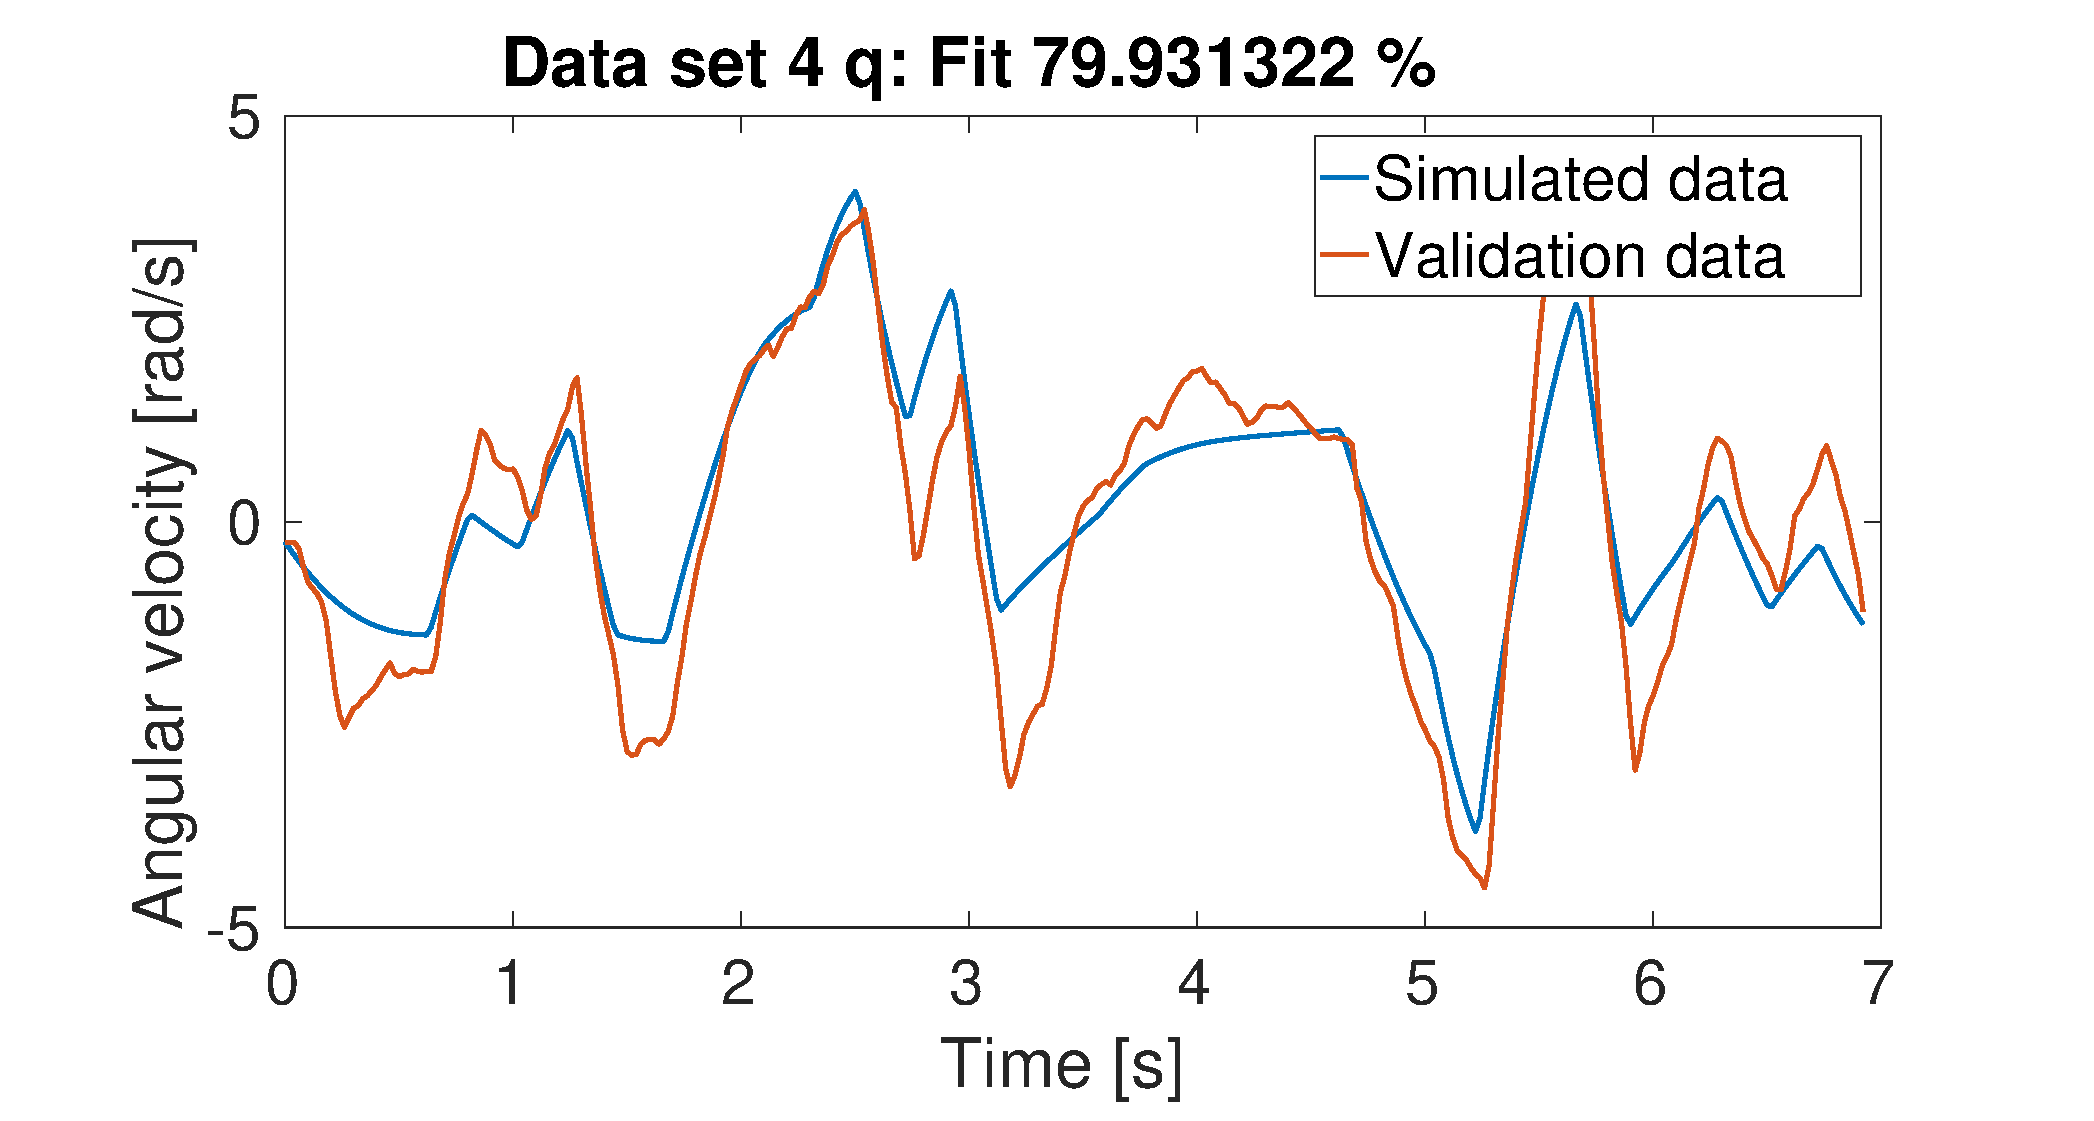
\includegraphics[width=0.7\textwidth]{ResultKalmanFixedMomentQ}}
  \\
  \subfloat[][Comparison between a simulated model response and validation data in $r$.]{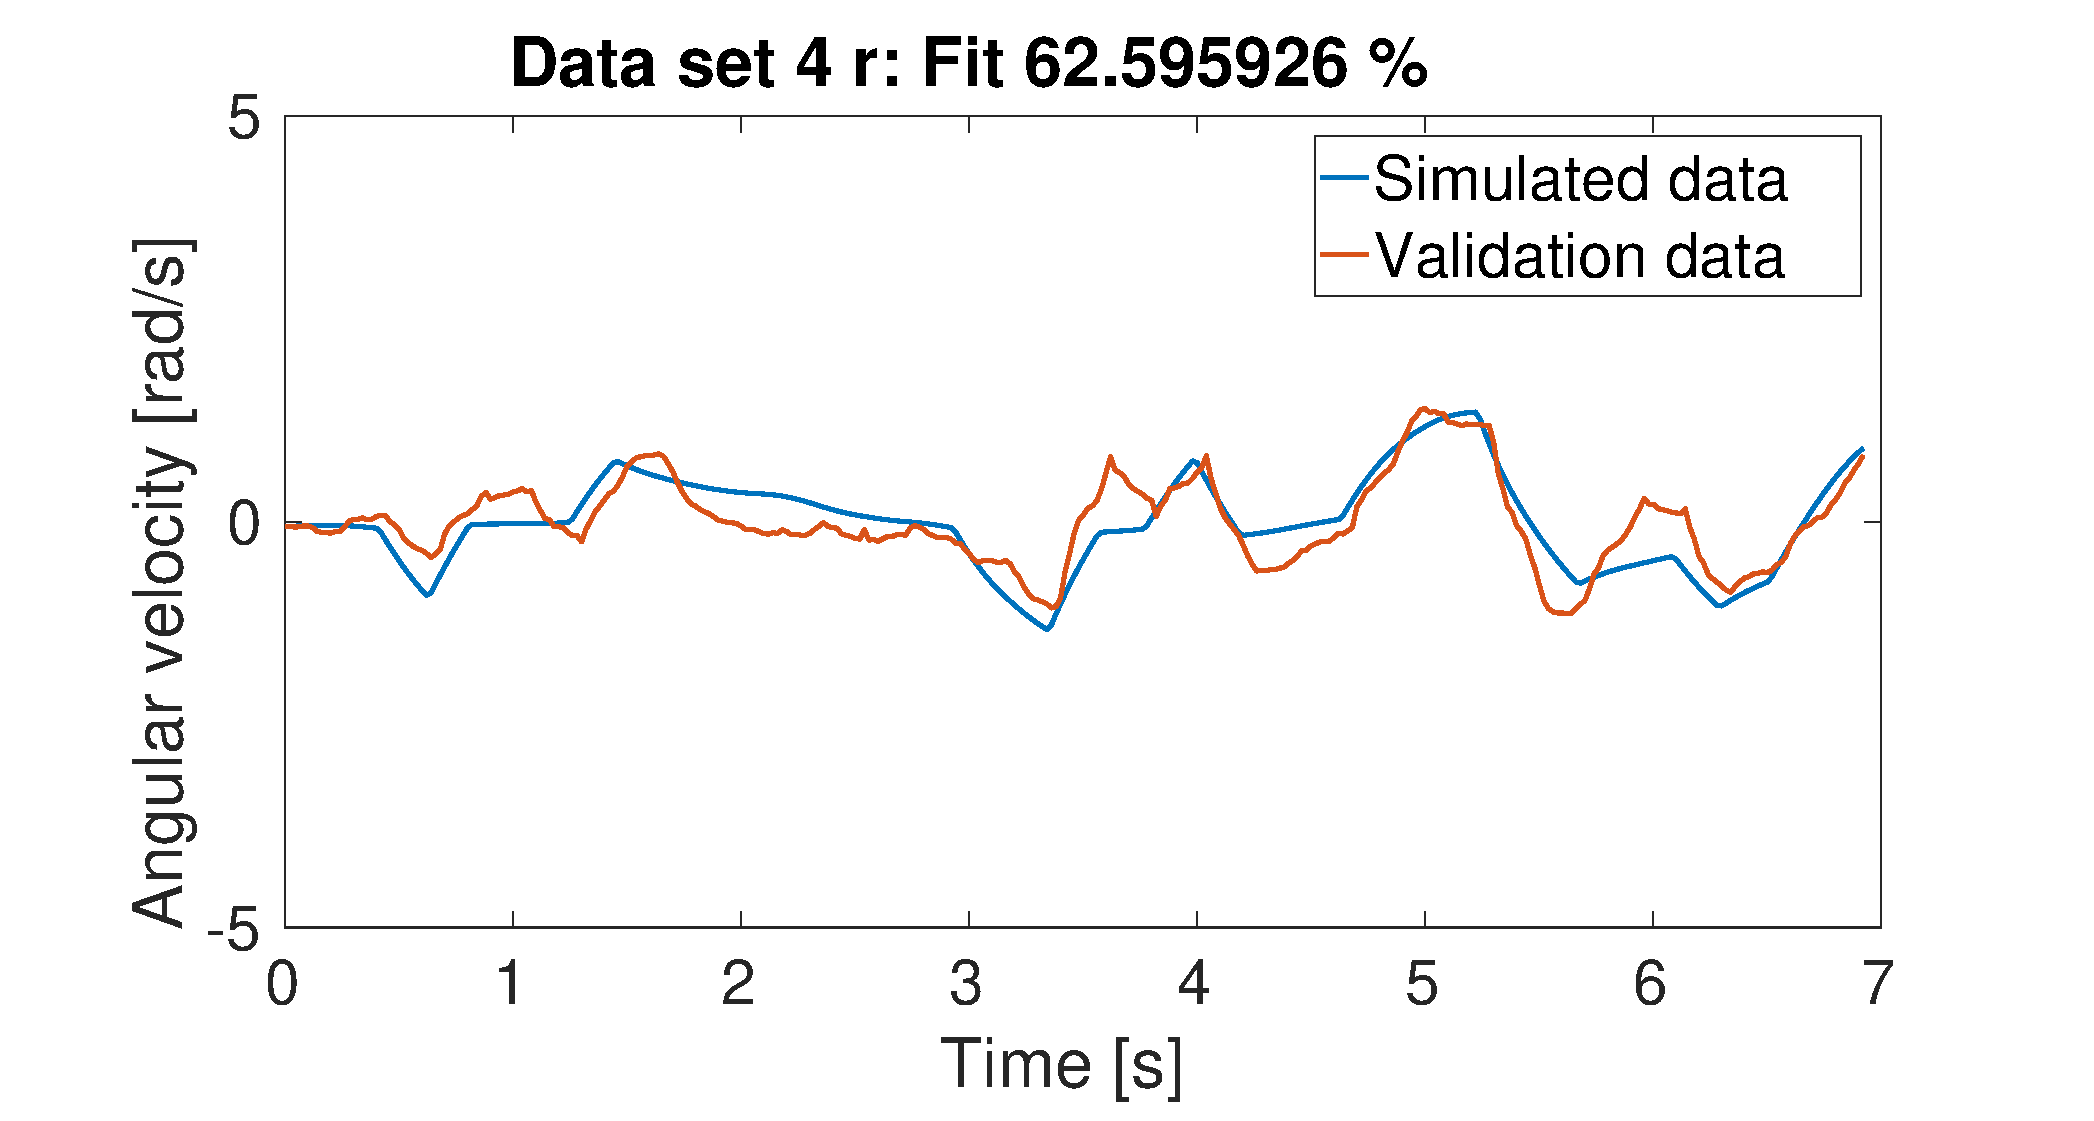
\includegraphics[width=0.7\textwidth]{ResultKalmanFixedMomentR}}
  \caption{\label{fig:ResultKalmanFixedMomentArms}%
    Comparison between simulation of $\nuVector$ (blue) with validation data (red). Moment-arm parameters are fixed. Goodness of fit statistic is displayed at the top of each sub-figure. The model describe the validation data well in $q$ and $r$ which can be seen in the high fit. The low fit in $p$ means that the model do not describe the validation data well.}
\end{figure}

A second estimation was run using same model with the following settings
\begin{equation*}
\boldsymbol{Q}=\text{diag}[\underbrace{\overbrace{100}^{\times4}}_{\etaVector}... \underbrace{\overbrace{1000}^{\times3}}_{\nuVector}...\underbrace{\overbrace{0.01}^{\times3}}_{\boldsymbol{b}}... \underbrace{\overbrace{0.01}^{\times10}... \overbrace{0.000001}^{\times5}}_{\boldsymbol{\theta}}]\text{ ,}
\end{equation*}
\begin{equation*}
\boldsymbol{R} = \text{diag}[\underbrace{\overbrace{0.001}^{\times3}}_{\text{Gyro}}... \underbrace{\overbrace{0.1}^{\times3}}_{\text{Acc}}... \underbrace{\overbrace{100}^{\times3}}_{\text{mag}}]
\end{equation*}
The estimation was done with three data sets, of which the first two were used for estimation and the third for validation. Since these datasets were shorter the estimator was iterated five times, using the parameter values from the previous iteration as the new initial states. The resulting parameter values and their initial values can be viewed in \tableref{tab:ResultKalmanFixedMomentArmsLz6} and a comparison of a simulated run against validation data is shown in \figureref{fig:ResultKalmanFixedMomentArmsLz6}

% results kalman lz6=0 fixed moment arms
\begin{table}[hbp]
  \centering
  \caption{\label{tab:ResultKalmanFixedMomentArmsLz6}%
    The estimated parameters from the Kalman estimator method with moment arms fixed to measured values but with $\distance{z}{6}$ fixed to zero.}
  \begin{tabular}{l l p{0.25\linewidth}}
    \toprule%
    \textbf{Notation}  & \textbf{Starting Value} & \textbf{Estimated Value} \\
    \otoprule%   
    % Parameters that will be estimated
    $\etaVector$			&$[1\ 0\ 0\ 0]^T$					&\\
    $\nuVector$			&$[0\ 0\ 0]^T$						&\\
    $\boldsymbol{b}$					&$[0\ 0\ 0]^T$			&\\
	$z_B$               & -0.05	\meter 						& -0.0606  	\meter\\
    $\Kp$               & -1   	\kilogram\usk\meter\squared 	& -0.8745 		\kilogram\usk\meter\squared\\
    $\Kpabsp$           & -1  	\kilogram\usk\meter\squared	& -0.6279  		\kilogram\usk\meter\squared\\
    $\Mq$               & -1  	\kilogram\usk\meter\squared	& -0.8529  		\kilogram\usk\meter\squared\\
    $\Mqabsq$           & -1  	\kilogram\usk\meter\squared	& -0.2505  	\kilogram\usk\meter\squared\\
    $\Nr$               & -1  	\kilogram\usk\meter\squared	& -1.0469		\kilogram\usk\meter\squared\\
    $\Nrabsr$           & -1  	\kilogram\usk\meter\squared	& -1.0405 		\kilogram\usk\meter\squared\\
    $A_p$               & 1 	\kilogram\usk\meter\squared	&  0.9728 		\kilogram\usk\meter\squared\\
    $B_q$               & 1 	\kilogram\usk\meter\squared	&  0.7266		\kilogram\usk\meter\squared\\
    $C_r$               & 1 	\kilogram\usk\meter\squared	&  1.2013		\kilogram\usk\meter\squared\\
    $\distance{x}{1}$  &0.19 \meter & 0.19 \meter\\
    $\distance{y}{1}$  &0.11 \meter & 0.1102 \meter\\
    $\distance{x}{2}$  &0.19 \meter & 0.19 \meter\\
    $\distance{y}{2}$  &0.11 \meter & 0.1102 \meter\\
    $\distance{y}{3}$  &0.11 \meter & 0.11 \meter\\
    $\distance{x}{5}$  &0.17 \meter & 0.1701 \meter\\
    $\distance{y}{4}$  &0.11 \meter & 0.11 \meter\\
    $\distance{z}{6}$  &0.0 \meter & 0.0 \meter\\ 
    \bottomrule%
  \end{tabular}
\end{table}

% results kalman lz6=0 fixed moment arms
\begin{figure}[tbp]
  \centering
  \subfloat[][Comparison between a simulated model response and validation data in $p$.]{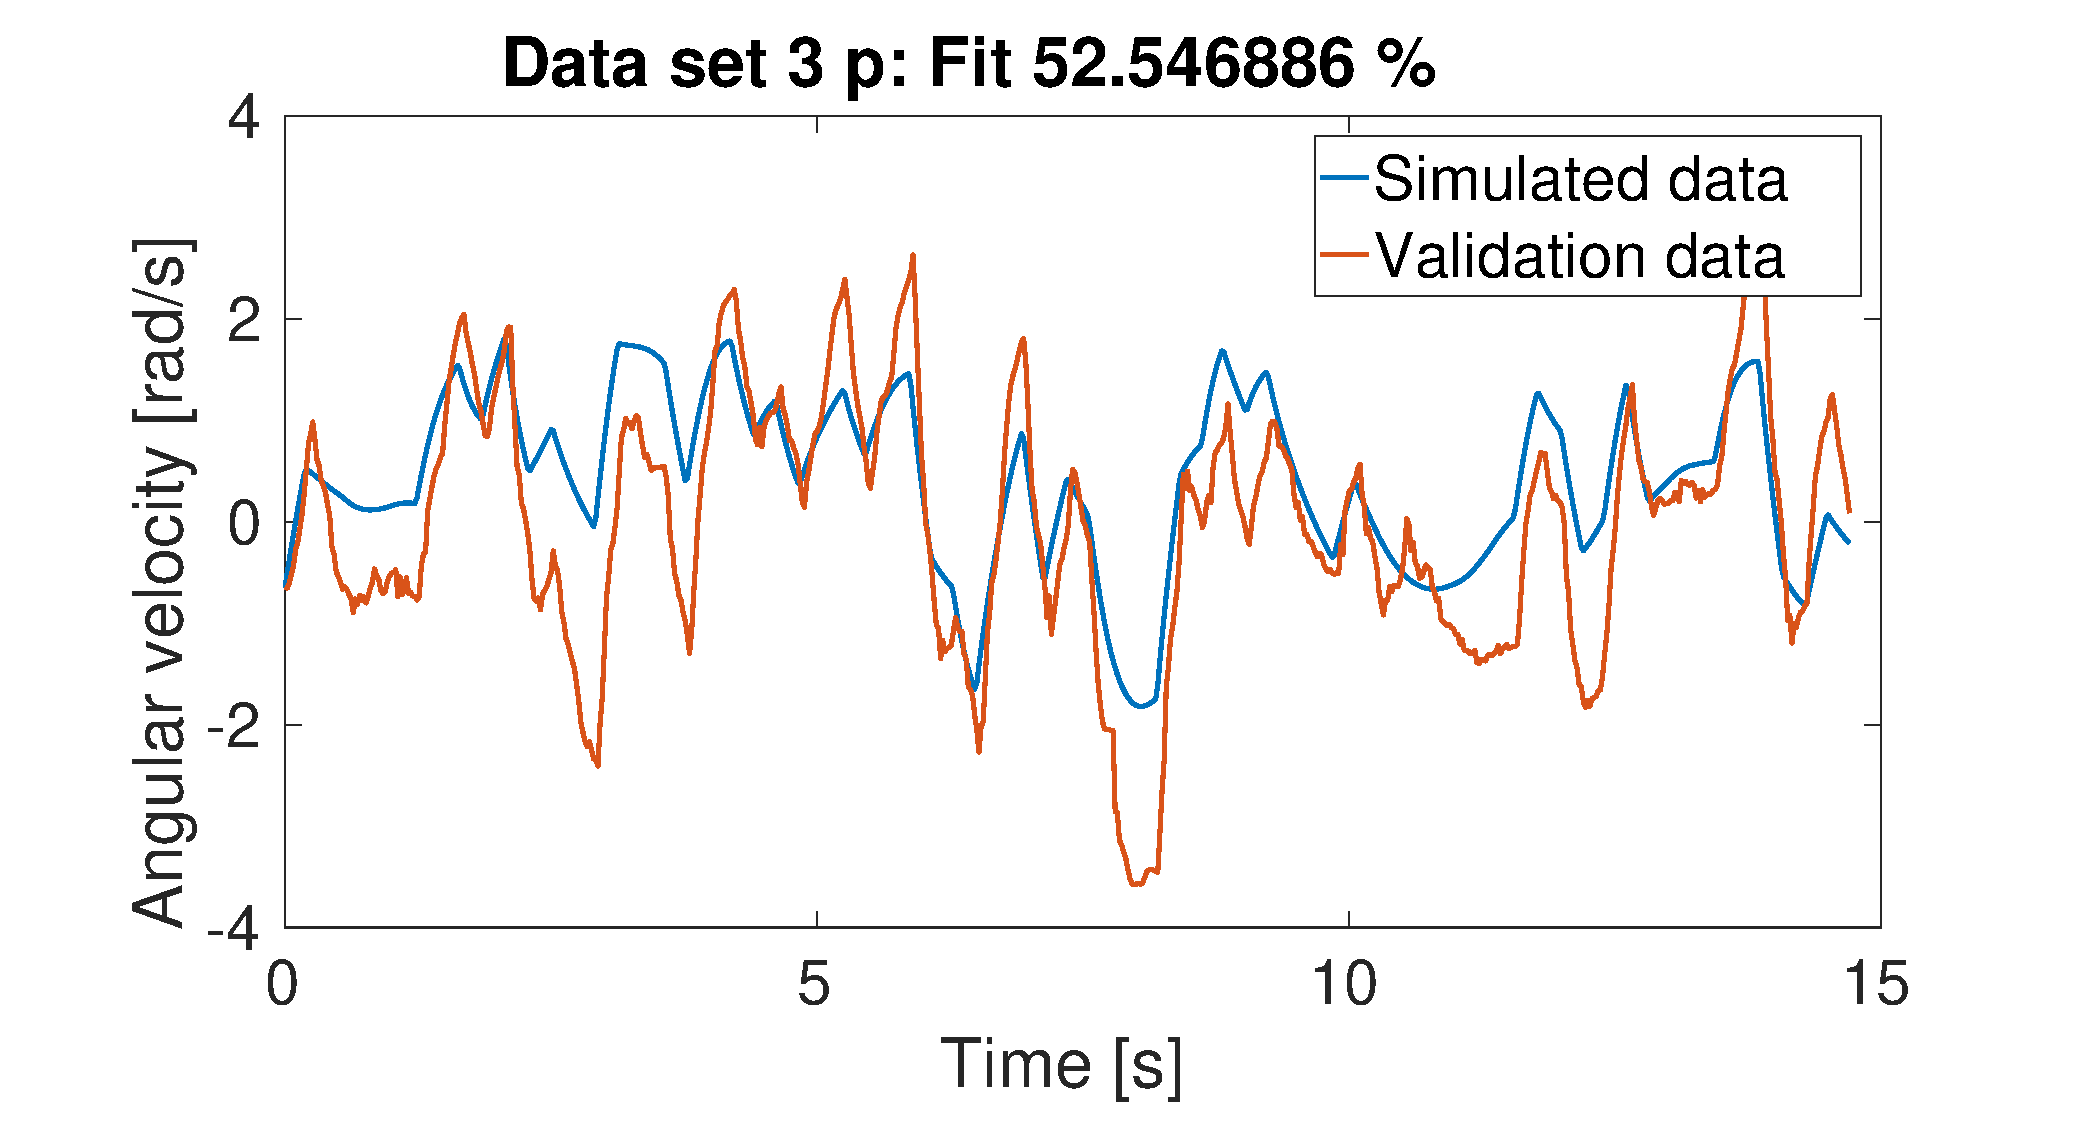
\includegraphics[width=0.7\textwidth]{ResultKalmanFixedMomentPLz0}}
  \qquad
  \subfloat[][Comparison between a simulated model response and validation data in $q$.]{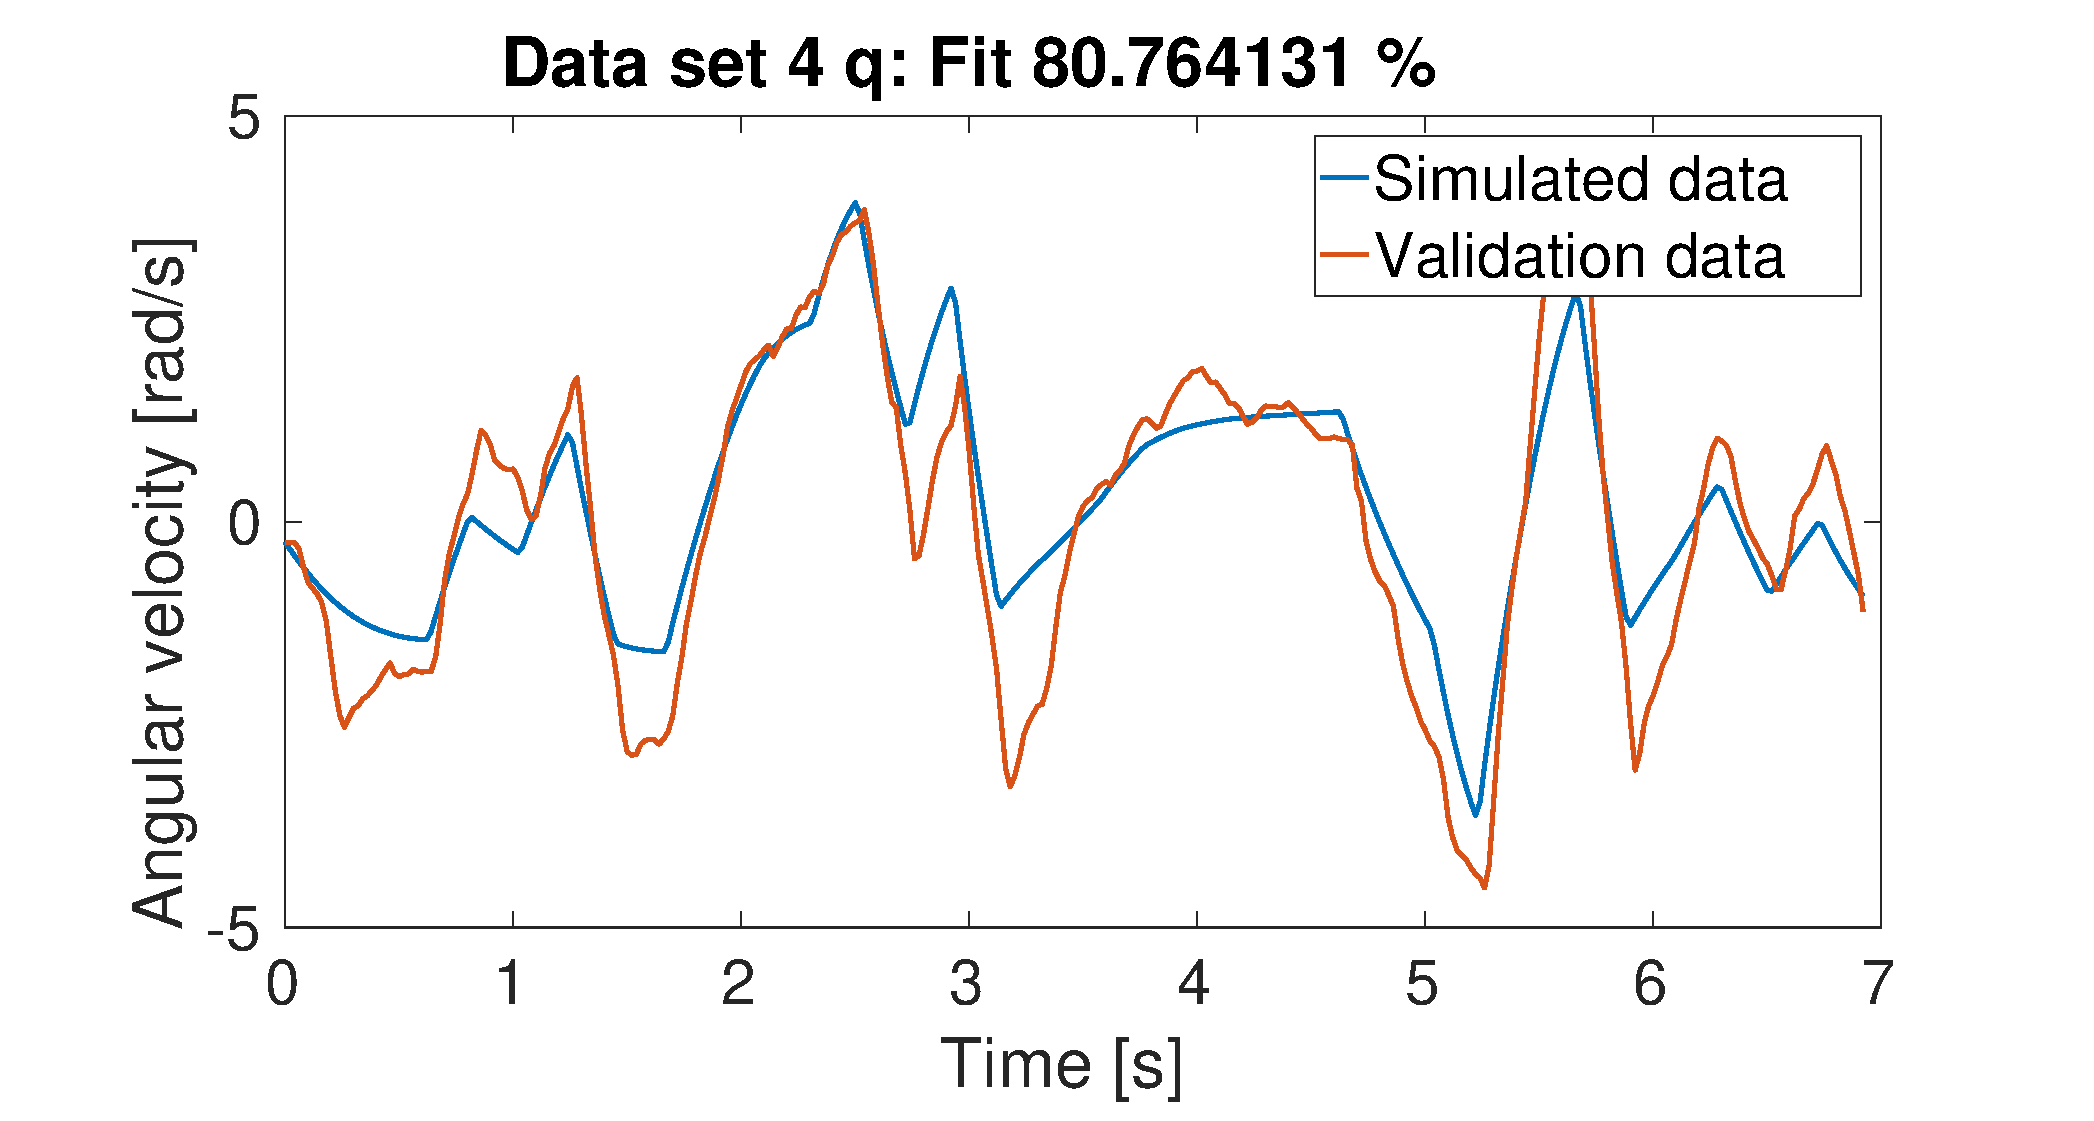
\includegraphics[width=0.7\textwidth]{ResultKalmanFixedMomentQLz0}}
  \\
  \subfloat[][Comparison between a simulated model response and validation data in $r$.]{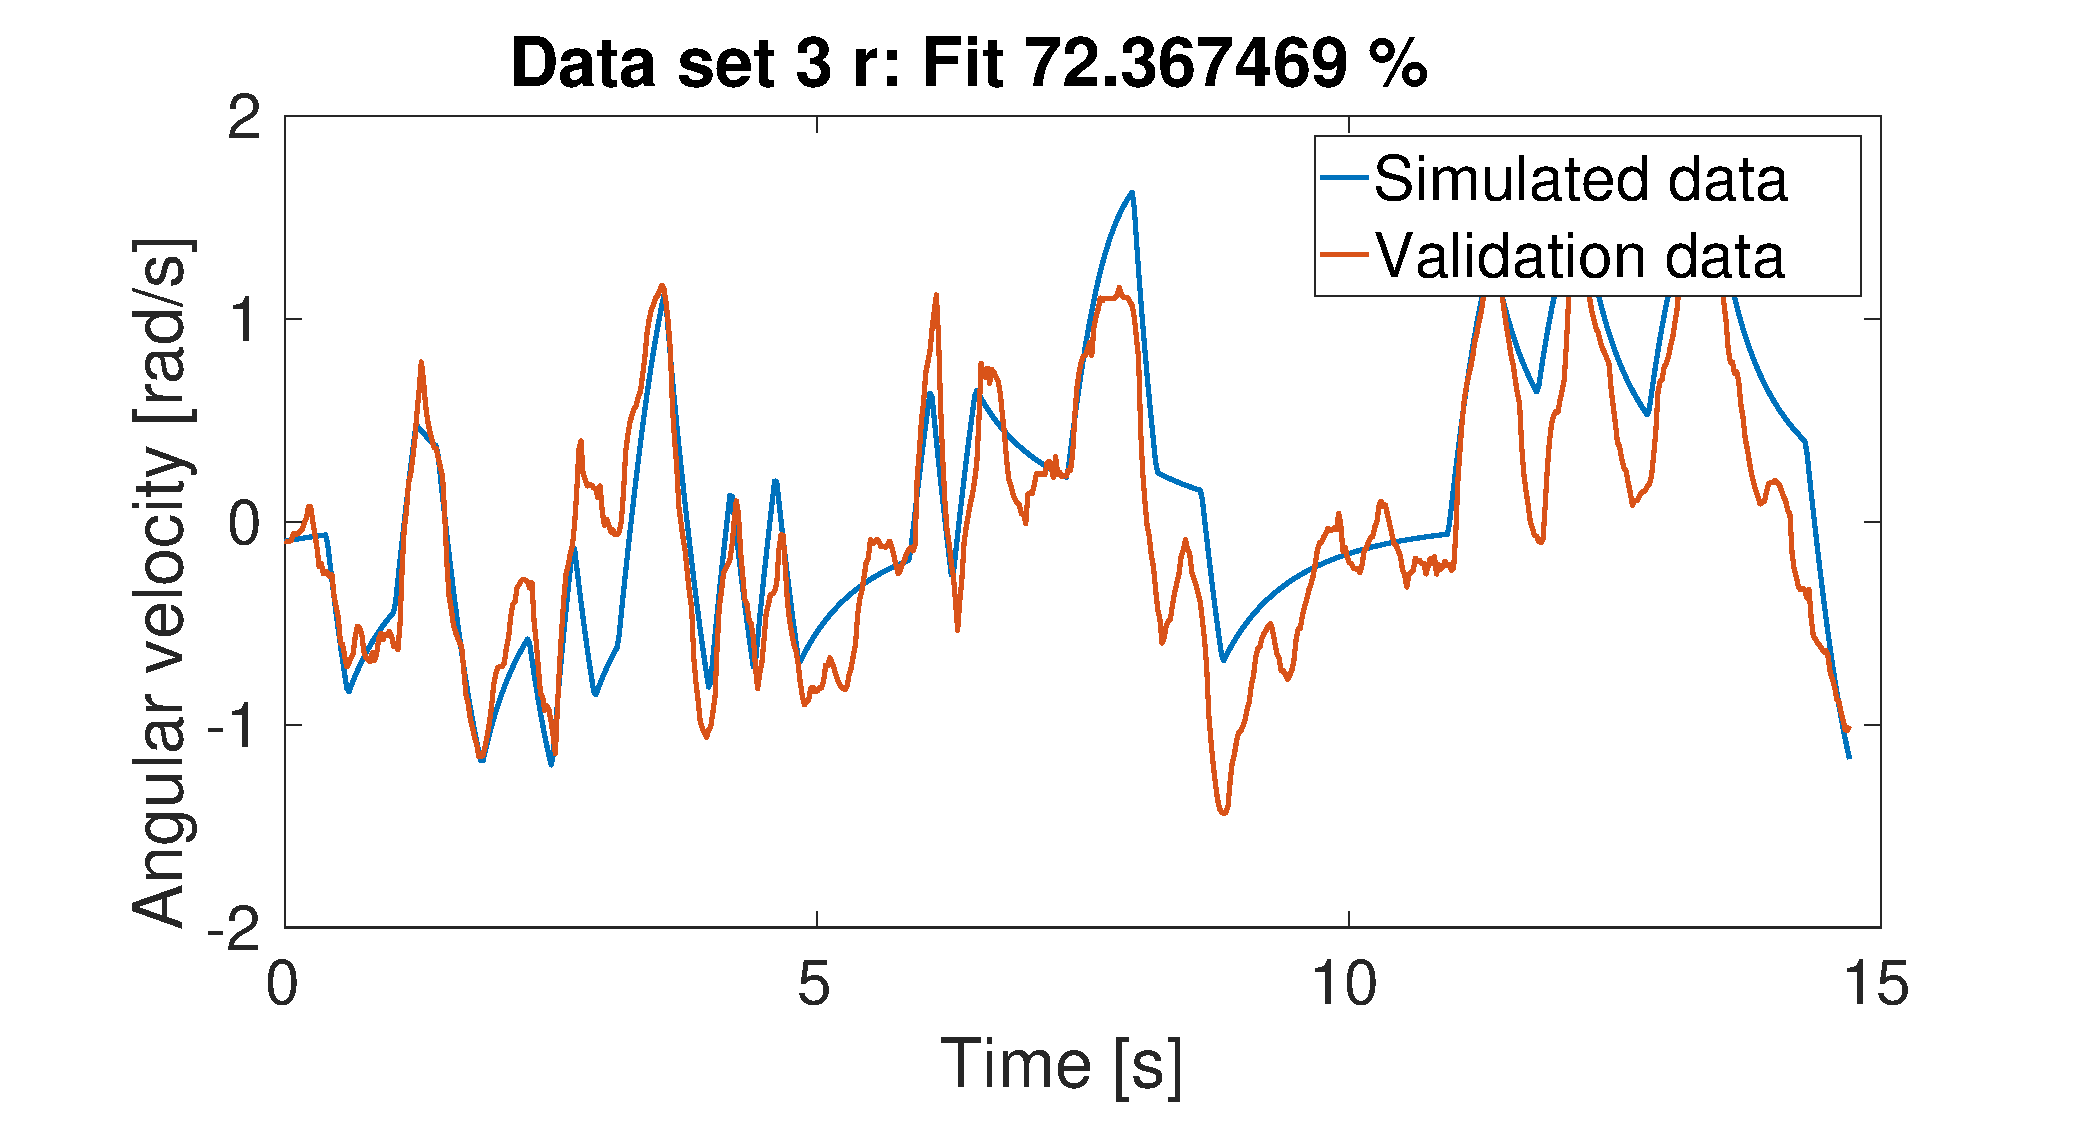
\includegraphics[width=0.7\textwidth]{ResultKalmanFixedMomentRLz0}}
  \caption{\label{fig:ResultKalmanFixedMomentArmsLz6}%
    Comparison between simulation of $\nuVector$ (blue) with validation data (red). Moment-arm parameters are fixed and \distance{z}{6} is set to zero. Goodness of fit statistic is displayed at the top of each sub-figure.}
\end{figure}


\section{Discussion}
To estimate parameters in the reduced 6-\abbrDOF model was harder than it at first seemed. Problems were encountered when the prediction-error method was used with bad fit in $p$. 





A problem that was consistent in all early attempts was a low fit value in $p$. Several adjustments were attempted in order to fix this issue and it was later found that the effect in $p$ of thruster 6 was minimal. A test showed that thruster 6 effected $p$ the most when it was quickly actuated. The effect of thruster 6 in $p$ can be seen in \Figureref{fig:thruster6}. If the sixth thrusters power was incremented slowly an initial response in $p$ was noted before it settled at zero again. This might be because of unmodelled translational dynamics of the \abbrROV meaning that the dynamics in $y$ may be coupled with $r$ or that the placement of \abbrCG in the \abbrROV is faulty. Thruster 6 also effected $r$, this can be due to unmodelled water interaction.

When deciding on which parameters to use for controller design, the choice was based solely on the fit of the simulated output had against validation data. The reasoning behind this being quite simple, the better the fit against validation data the less robust the controllers would have to be.


\begin{figure}
\centering
  \subfloat[][\label{fig:thruster6p1} The effect in $p$ when only using thruster 6.]{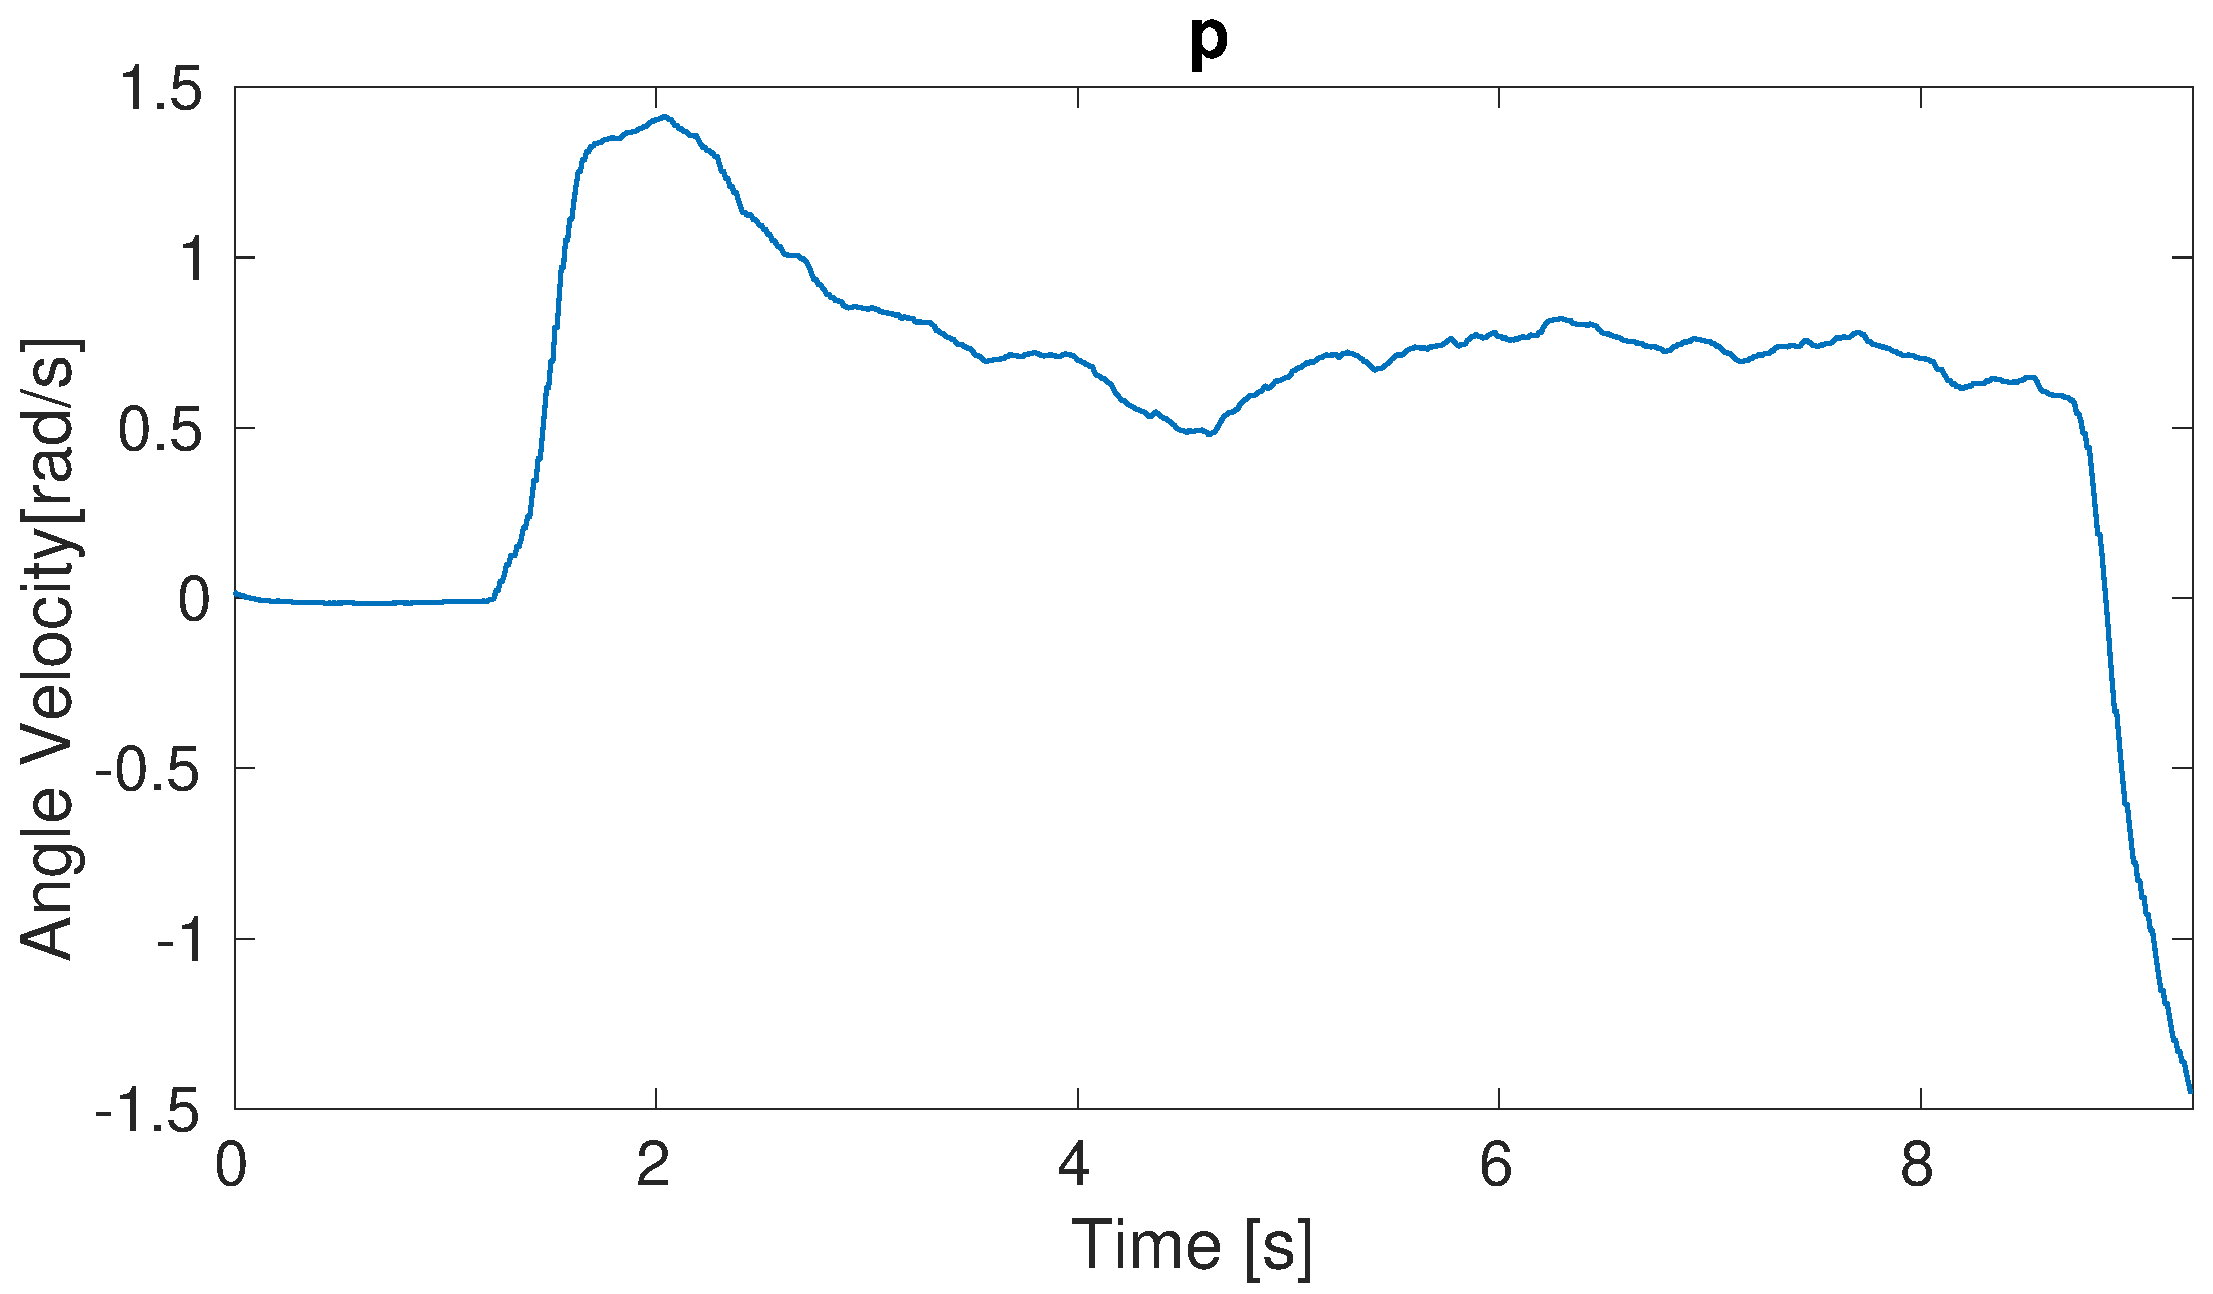
\includegraphics[width=0.4\textwidth]{thruster6p}}
  \qquad
  \subfloat[][\label{fig:thruster6u61} The effect in $r$ when only using thruster 6.]{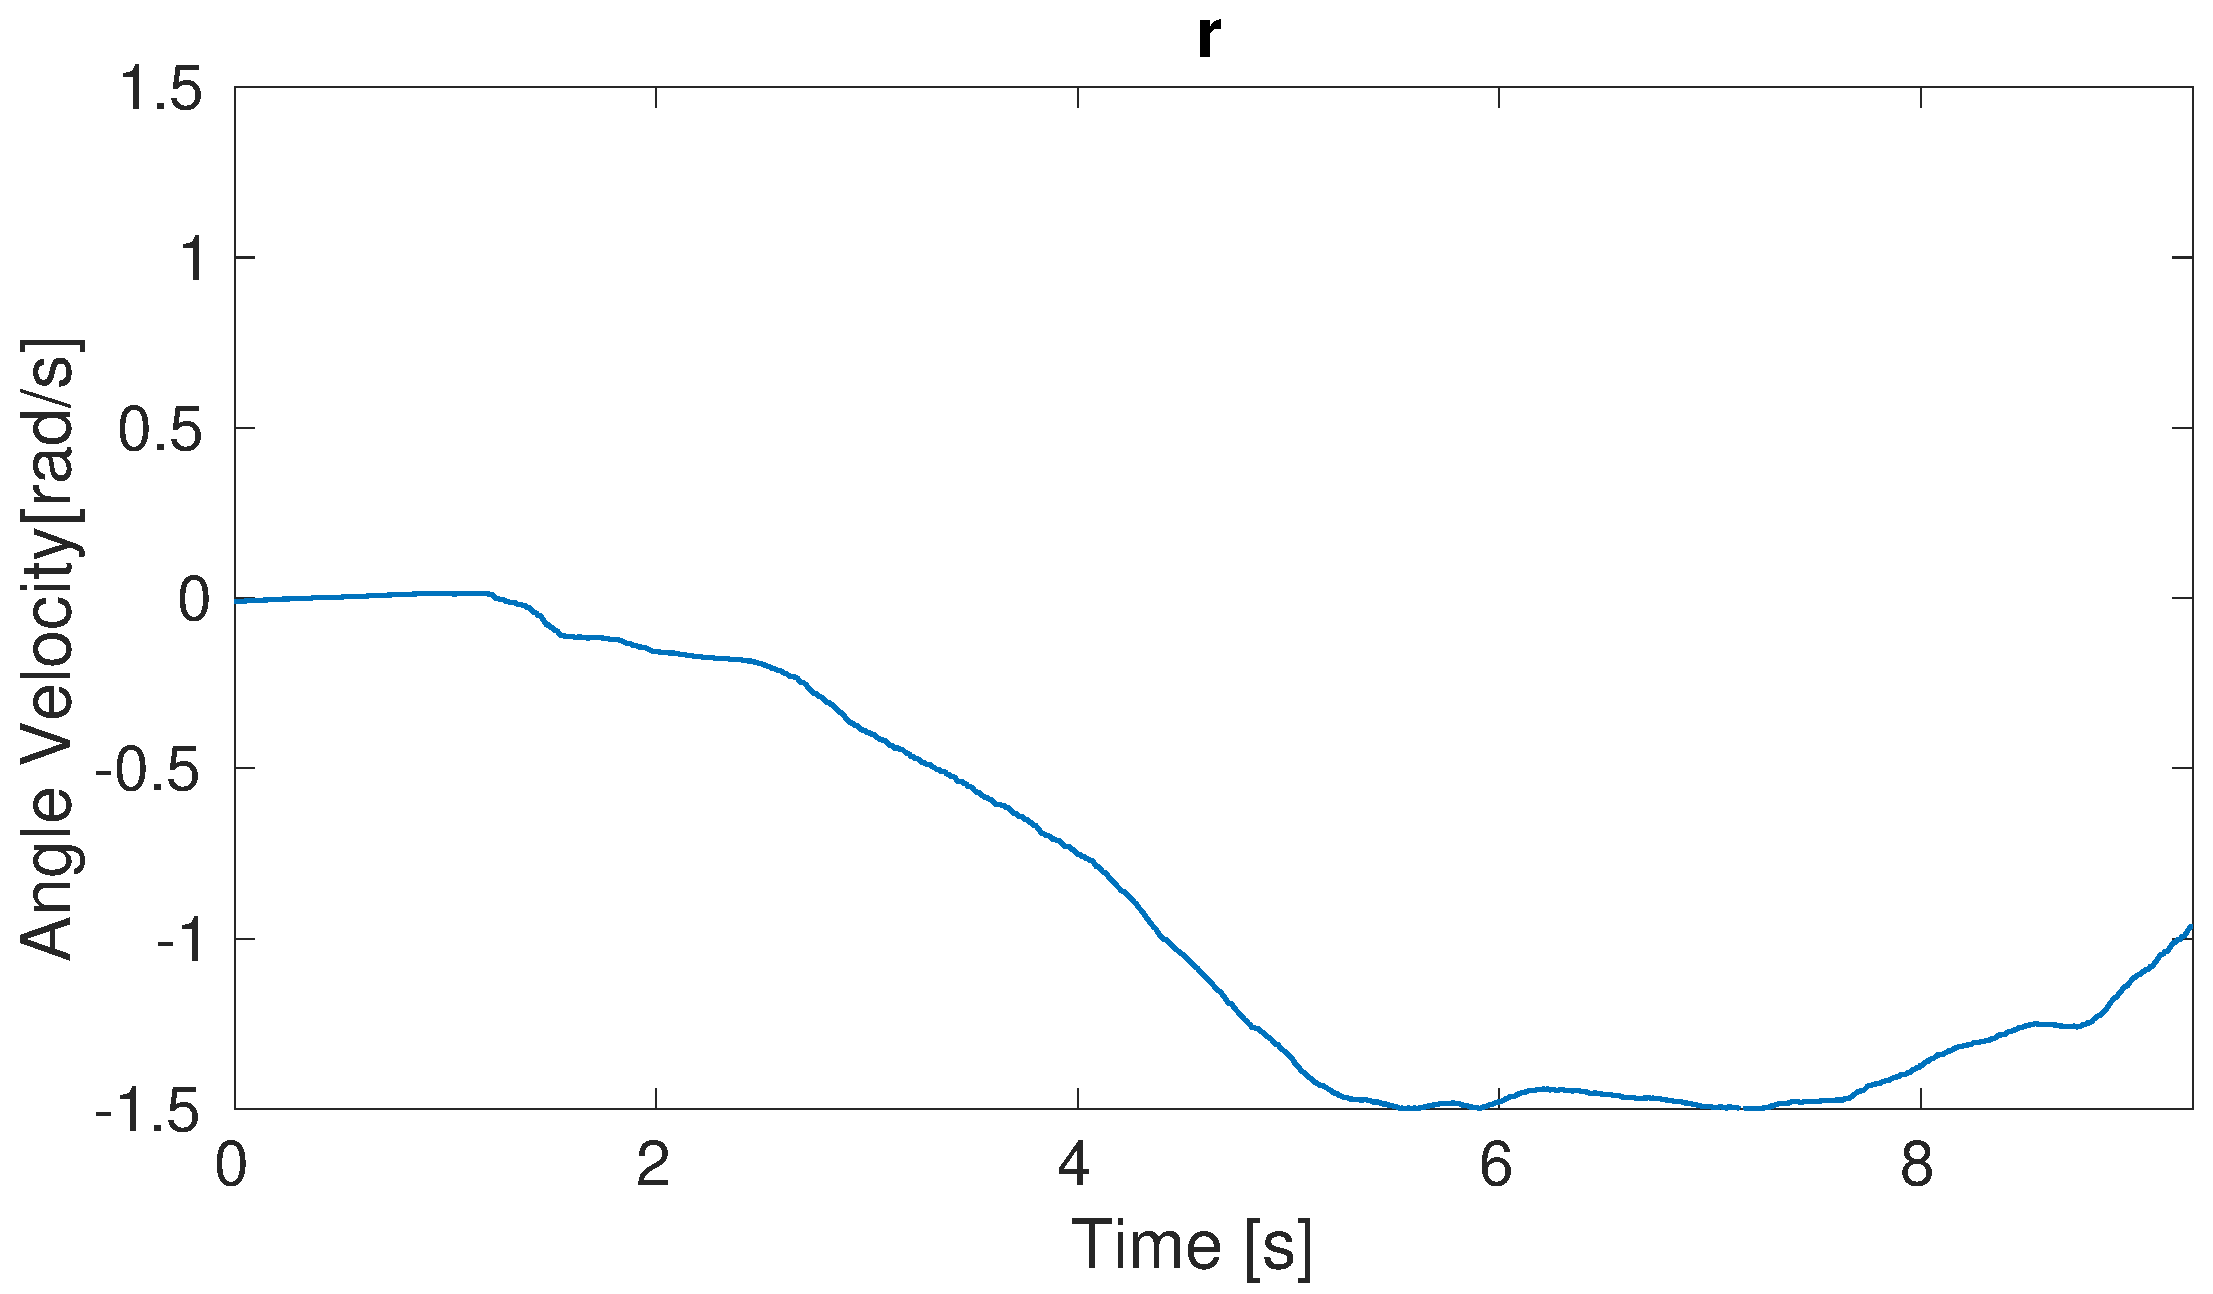
\includegraphics[width=0.4\textwidth]{thruster6r}}
  \qquad
  \subfloat[][\label{fig:thruster6r1} The control signal sent to thruster 6.]{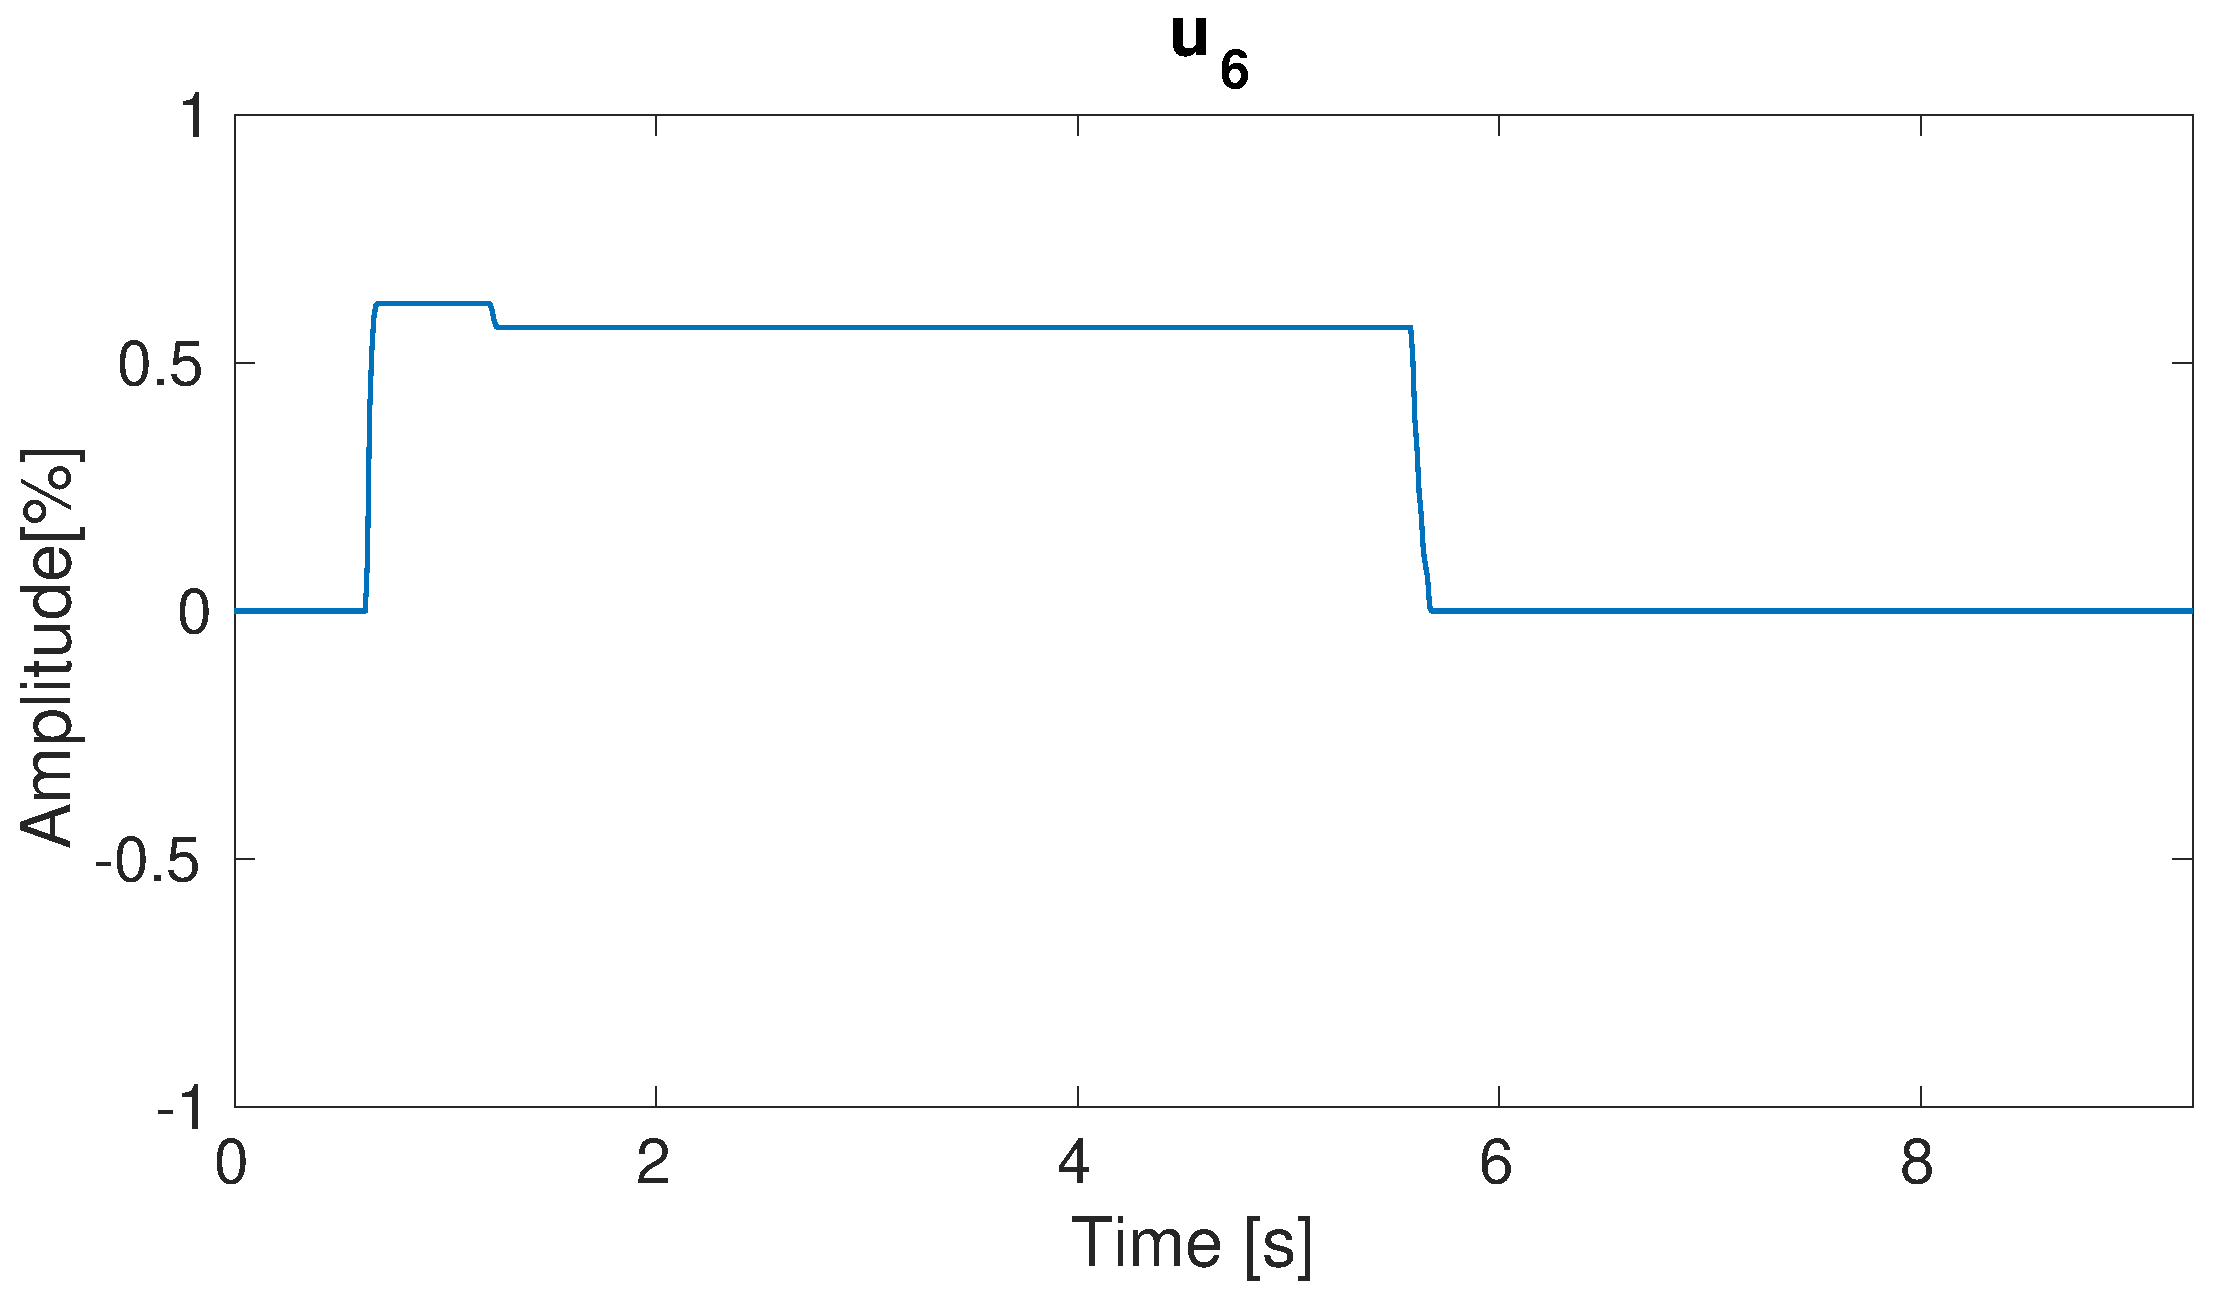
\includegraphics[width=0.4\textwidth]{thruster6u6}}
  \caption{\label{fig:thruster6}%
  The effect in $p$ and $r$ while only using thruster 6. As can be seen thruster 6 has a relatively small effect in $p$, thus ought the moment arm of thruster 6 be small. However, thruster 6 effected $p$ more when thruster 6 was quickly actuated.}
\end{figure}

%%%%%%%%%%%%%%%%%%%%%%%%%%%%%%%%%%%%%%%%%%%%%%%%%%%%%%%%%%%
%\section{Decoupling the Model} \index{Decoupling}
% From \eqref{eq:WithoutTranslation} it can be seen that $r$ is not affected by the same thrusters as $p$ and $q$. Thus the $r$ model's parameters were initially estimated by themselves while the parameters in the $p$ and $q$ models were estimated together. 
%
%The estimation of the attitude model structure was divided into three estimation steps.
%
%The separately estimated parameters were then used as starting values for a complete attitude model parameter estimation, \eqref{eq:WithoutTranslation}. The reduced models for $r$, $p$ and $q$ that were used during initial estimation were
%
%The simplification could be done since excitation in the states not used in a particular estimation were kept at a minimum during data collection. Thus the coupled terms in each equation were approximated to be zero.

%%%%%%%%%%%%%%%%%%%%%%%%%%%%%%%%%%%%%%%%%%%%%%%%%%%%%%%%%%%
%\section{Parameter Estimation from Angular Velocities} \label{sec:estimation_angular}
%The estimated Euler angles from the sensor fusion model described in \Sectionref{sec:simple_model} did not follow the kinematic relation described in \Sectionref{sec:kinematics} which can be seen in \Figureref{fig:integratedAngleVelocities}. This also meant that the angles were unfit for use in as outputs in the parameter estimation since the angle estimates will not describe the system well since the estimates include the \abbrEKF's dynamics. The parameters were instead estimated using the angular velocities from the gyroscope as outputs an with the estimated euler angles as inputs. The model structure in which the parameters were estimated was thus \index{model structure}
%\begin{equation}
%\etaVectordot = f(\nuVector, \hat{\etaVector}, \tauVector),
%\end{equation}
%and
%\begin{equation}
%\boldsymbol{y} = \nuVector
%\end{equation}
%where $\hat{\etaVector}$ contains the estimated Euler angles from the sensor fusion.
%
%
%
%To get an initial estimate on the parameters in the yaw dynamics the reduced model parameters in \eqref{eq:r_dot_decouple}
%were estimated using data collected from a test that mainly excited the \abbrROV in $r$ which can be seen in \Figureref{r_rTest}.
%
%Since the dynamics in $p$ and $q$ are coupled \eqref{eq:pq_dot_decouple1} and \eqref{eq:pq_dot_decouple2} needed to be estimated at the same time. The cross terms in $r$ was assumed to be zero since the \abbrROV was mainly excited in $p$ and $q$ during collection of the used estimation data which can be seen in \Figureref{p_qTest}.
%
%The initial estimates of the parameters in \eqref{eq:pq_dot_decouple1} and \eqref{eq:r_dot_decouple} were used as initial estimates of the parameters in \eqref{eq:WithoutTranslation}. Due to observational problems the reparametrisation $A_p = \Ix - \Kpdot$, $B_q = \Iy - \Mqdot$ and $C_r = \Iz - \Nrdot$ was introduced. The fit can be seen in \Figureref{fig:velocityCompareCong} where the reparameterisation has been used.
%\index{Reduced model structure}
%
%%%%%%%%%%%%%%%%%%%%%%%%%%%%%%%%%%%%%%%%%%%%%%%%%%%%%%%%%%%%
%\section{Parameter Estimation from Angular Velocities and Linear Accelerations} \label{sec:angLinEstim}
%The parameters were also estimated using the angular velocities and the linear accelerations as outputs. This was done to avoid modelling the low-pass filtering effects in the sensor fusion described in \Chapterref{cha:sensor_fusion}. The model structure was modified to use quaternions instead of euler angles. Using quaternions in the model \eqref{eq:p_dotWithoutTranslation} - \eqref{eq:r_dotWithoutTranslation} with the reparameterision from \Sectionref{sec:estimation_angular} gave the model structure \todo{move model def to model chapter}
%\begin{multline}
%\pdot = \frac{\thrusterfun{1} \distance{y}{1} - \thrusterfun{2} \distance{y}{2} + \thrusterfun{6} \distance{z}{6}}{A_p} + \frac{B z_B (2 \quatII \quatIII + 2 \quatI \quatO)}{A_p} + \\ \frac{p (\Kp + \Kpabsp \abs{p})}{A_p} + \frac{q r (B_q - C_r)}{A_p},
%\end{multline}
%\begin{multline}
%\qdot = \frac{\thrusterfun{1} \distance{x}{1} + \thrusterfun{2} \distance{x}{2} - \thrusterfun{5} \distance{x}{5}}{B_q} - \frac{B z_B (2 \quatI \quatIII - 2 \quatII \quatO)}{B_q} + \\ \frac{q (\Mq + \Mqabsq \abs{q})}{B_q} - \frac{p r (A_p - C_r)}{B_q}
%\end{multline}
%and
%\begin{multline}
%\rdot = \frac{\thrusterfun{3} \distance{y}{3} - \thrusterfun{4} \distance{y}{4}}{C_r} + \frac{r (\Nr + \Nrabsr \abs{r}}{C_r} + \frac{p q (A_p  - B_q)}{C_r}
%\end{multline}
%
%Thus the model structure in which the parameters was estimated became \index{model structure}
%\begin{equation}
%\etaVectordot = J(\etaVector) \nuVector,
%\end{equation}
%\begin{equation}
%\dot{\nuVector} =  f(\etaVector, \nuVector, \tauVector)
%\end{equation}
%with 
%\begin{equation}
%\boldsymbol{y} = \begin{pmatrix}
%\etaVector \\
%\boldsymbol{a}
%\end{pmatrix}
%\end{equation}
%where $\boldsymbol{a}$ are the linear accelerations in the \abbrROV frame. 
%
%The fit of the model compared to validation data can be seen in \Figureref{fig:angVelCompare}. To properly estimate the parameters the initial states had to be well estimated. The importance of a correct initial state estimate can be seen in \Figureref{fig:angVelSim}. Here the estimator was fed simulated data and was initialised with the true parameter values but had to estimate the starting state.   The estimated starting state was not well estimated, which in turn led to the parameters diverging from the true parameters and a low fit. A Kalman smoother as described in \citet{Wallin} was used introduced in order to alleviate this problem. During initial state estimation using the Kalman smoother the magnetometer was added as a output to reduce the uncertainty of the initial quaternions.
%
%
%To handle noisy signals an error threshold was introduced. An error threshold means that after a breakpoint the cost function becomes linear instead of quadratic. This makes the parameter estimation less sensitive to outliers. To reduce the impact of the noise even further the used weight matrix in the cost function was the inverse of the estimated noise covariance. 

%%%%%%%%%%%%%%%%%%%%%%%%%%%%%%%%%%%%%%%%%%%%%%%%%%%%%%%%%%%%
\section{Estimated Parameters}\label{sec:parameterResults}
\Tableref{tab:parameterConstants} shows the know, measured and estimated parameters used in the \abbrROV and controller development.

\begin{table}[tbp]
  \centering
  \caption{\label{tab:parameterConstants}%
    The known and estimated parameters used in the \abbrROV model.}
  \begin{tabular}{l l p{0.58\linewidth}}
    \toprule%
    \textbf{Notation}   & \textbf{Value} & \textbf{Description} \\
    \otoprule%
    $m$                 & 6.621 \kilogram                    & Mass of the \abbrROV. \\            
    $g$                 & 9.82  \meter\per\second\squared    & Gravity acceleration.\\   
    $\rho$              & 1000  \kilogram\per\meter\cubed    & Density of water.\\       
    
    $\distance{x}{1}$   & 0.19 \meter & Distance from \abbrCG to thruster 1 in $\xPosition$-direction.\\
    $\distance{y}{1}$   & 0.11 \meter & Distance from \abbrCG to thruster 1 in $\yPosition$-direction.\\
    $\distance{y}{2}$   & 0.11 \meter & Distance from \abbrCG to thruster 2 in $\yPosition$-direction.\\
    $\distance{x}{2}$   & 0.19 \meter & Distance from \abbrCG to thruster 2 in $\xPosition$-direction.\\
    $\distance{y}{3}$   & 0.11 \meter & Distance from \abbrCG to thruster 3 in $\yPosition$-direction.\\
    $\distance{x}{5}$   & 0.17 \meter & Distance from \abbrCG to thruster 5 in $\xPosition$-direction.\\
    $\distance{y}{4}$   & 0.11 \meter & Distance from \abbrCG to thruster 4 in $\yPosition$-direction.\\
    $\distance{z}{6}$   & 0    \meter & Distance from \abbrCG to thruster 6 in $\zPosition$-direction.\\
    	$z_B$               & -0.0331 \meter                                      & Distance from \abbrCG to \abbrCB.\\
    $\Kp$               & -0.8325 \kilogram\usk\meter\squared                 & Linear damping coefficient due to rotation in water about the $\xPosition$-axis.\\
    $\Kpabsp$           & -0.4933 \kilogram\usk\meter\squared                 & Quadratic damping coefficient due to rotation in water about the $\xPosition$-axis.\\
    $\Mq$               & -0.8487 \kilogram\usk\meter\squared                 & Linear damping coefficient due to rotation in water about the $\yPosition$-axis.\\
    $\Mqabsq$           & -0.2507 \kilogram\usk\meter\squared                 & Quadratic damping coefficient due to rotation in water about the $\yPosition$-axis.\\
    $\Nr$               & -1.7580 \kilogram\usk\meter\squared                 & Linear damping coefficient due to rotation in water about the $\zPosition$-axis.\\
    $\Nrabsr$           & -1.4595 \kilogram\usk\meter\squared                 & Quadratic damping coefficient due to rotation in water about the $\zPosition$-axis.\\
    $A_p$               & 0.6024  \kilogram\usk\meter\squared                 & Inertia around the $\xPosition$-axis and increased inertia around the $\xPosition$-axis.\\
    $B_q$               & 0.7834  \kilogram\usk\meter\squared                 & Inertia around the $\yPosition$-axis and increased inertia around the $\yPosition$-axis.\\
    $C_r$               & 1.3993  \kilogram\usk\meter\squared                 & Inertia around the $\zPosition$-axis and increased inertia around the $\zPosition$-axis.\\
    \bottomrule%
  \end{tabular}
\end{table}